%% Copernicus Publications Manuscript Preparation Template for LaTeX Submissions
%% ---------------------------------
%% This template should be used for copernicus.cls
%% The class file and some style files are bundled in the Copernicus Latex Package, which can be downloaded from the different journal webpages.
%% For further assistance, please contact Copernicus Publications at: production@copernicus.org
%% https://publications.copernicus.org/for_authors/manuscript_preparation.html


%% 2-column papers and preprints
\documentclass[nhess, manuscript]{copernicus}
%\documentclass[nhess, twocol]{copernicus}


% Defining colours for the considered datasets
\usepackage{xcolor}
\definecolor{colourTraining}{HTML}{800080}
\definecolor{colourOuterFolds}{HTML}{888888}
\definecolor{colourOuterTest}{HTML}{2CA58D}
\definecolor{colourInnerTraining}{HTML}{FF0066}
\definecolor{colourInnerValidation}{HTML}{E98A15}
\definecolor{colourTest}{HTML}{00B0F0}


\begin{document}

\title{Medium-range data-driven hydro-meteorological predictions of areas at risk of flash flood (Part 1: regional model development)}

\Author[1,2][fatima.pillosu@ecmwf.int]{Fatima M. Pillosu}{} %% correspondence author
\Author[2]{Mariana Clare}{}
\Author[2]{Florian Pappenberger}{}
\Author[2]{Christel Prudhomme}{}
\Author[1,3]{Hanna Cloke}{}

\affil[1]{Department of Geography and Environmental Science, University of Reading, Whiteknights Campus, PO Box 227, Reading, RG6 6AB, UK}
\affil[2]{European Centre for Medium-range Weather Forecasts, Shinfield Rd, Reading, RG2 9AX, UK}
\affil[3]{Department of Meteorology, Brian Hoskins Building, University of Reading, Whiteknights Road, Earley Gate, Reading, RG6 6ET, UK}


\runningtitle{Data-driven hydro-meteorological predictions of areas at risk of flash flood (Part 1)}
\runningauthor{Fatima M. Pillosu}


%% These dates will be inserted by Copernicus Publications during the typesetting process.
\received{}
\pubdiscuss{} %% only important for two-stage journals
\revised{}
\accepted{}
\published{}


\firstpage{1}

\maketitle

\begin{abstract}
TEXT
\end{abstract}


\introduction  
Flash floods are sudden and severe events characterised by rapid water rise and high flow velocities, often triggered by intense localised rainfall (Wang et al., 2023). Due to the magnitude of economic damages and loss of life they cause, flash floods are among the most devastating natural disasters worldwide (Rentschler et al., 2022). The occurrence of extreme flash flood events such as those in Germany (Fekete and Sandhill, 2021; Thieken et al., 2023) and China in 2021 (Manandhar et al., 2023), Libya in 2023 (Hewson et al., 2024), and United Arab Emirates in 2024 (Oxford Analytica, 2024) exposes weaknesses in the management of this hazard, particularly in urban areas. It also highlights the need for a better understanding of the hazard and its associated risks to develop efficient early warning systems and enhance preparedness and emergency response to better protect people and livelihoods. Moreover, since flash-flood-triggering rainfall events are expected to increase in intensity and frequency by 2100 (Kotz et al., 2023; Thackeray et al., 2022), and the vulnerability to flooding of global population is increasing due to extensive urbanisation (Mazzoleni et al., 2022), it is paramount to protect people and infrastructure against future low-probability, high-impact or yet unseen flash flood events (Hewson, 2024; Montanari et al., 2024; Zhou et al., 2022). On 2022’s World Meteorological Day, the UN Secretary-General António Guterres announced the EarlyWarnings4All initiative to ensure every person on Earth is protected by early warning systems by 2027. The initiative’s Executive Action Plan highlights the importance of strengthening forecast capabilities for flash floods (WMO, 2022). 

The stochastic nature of flash floods makes forecasting specific events extremely challenging. The two most common approaches for flash flood prediction leverage nowcasting and numerical weather prediction (NWP) models. Nowcasting involves the use of real-time data from weather radars, satellites, and ground-based observations to provide very short-range forecasts of flash flood events (e.g., up to a few minutes to a few hours ahead). Nowcasting has gained significant attention in the context of flash flood forecasting, especially in urban areas, due to its potential to provide very accurate warnings, even though with very reduced lead time. The use of km-scale quantitative precipitation estimates such as in ERICHA rainfall nowcasts, has enhanced the overall predictive capabilities for flash floods, enabling more timely warnings (Park et al., 2019). Improvements in computational power allow to run, especially at city-scale, hydrodynamic models that can accurately represent the complex interactions between rainfall, surface runoff, and drainage systems (Xing et al., 2019). Such highly detailed predictions enable planners and emergency managers to assess flood risk, evaluate infrastructure vulnerabilities, and develop targeted strategies for flood resilience and adaptation. However, these models are very expensive to run for very large areas, so that their coverage worldwide is very patchy. The Flash Flood Guidance (FFG) provides a good efficient alternative to generate flash flood predictions for large regions. The FFG estimates the average amount of rainfall needed to trigger flash flooding in a specific catchment area. There is currently an effort to implement the FFG system worldwide. However, its current coverage of flash flood forecasting systems remains patchy. To have real global coverage, it would be good to have systems like the Global Flood Awareness System (GloFAS) that provides flood predictions over a continuous global domain. However, due to data and computational restrictions, such system is not able to provide guidance for small, flashy catchments. Data-driven approaches have shown to generate more accurate flood predictions than physically based models, at a fraction of the cost (Kratzert et al., 2023). For an overview of the rapid-changing landscape in data-driven flood forecasting, the reader is referred to the numerous review articles published in recent years in the peer-reviewed literature (Ghorpade et al., 2021; Karim et al., 2023; Khairudin et al., 2022; Kumar et al., 2023; Maspo et al., 2020; Rathnasiri et al., 2023). Feasibility studies on whether global data-driven models could be used also to predict flash floods are limited. At catchment level, data-driven models have shown the capability to predict accurately river discharge for small flashy catchments. However, their capability to do so at global scale remains poorly understood primarily due to the lack of observational data (for example, but not limited to rainfall, river discharge  timeseries and impact reports) required to model accurately rainfall-runoff processes (Malik et al., 2024; Zhao et al., 2022). Furthermore, such approaches have not tackled the issues related to the impacts that the underrepresentation of rainfall variability within the catchments has in the accuracy of flash flood predictions that has been long acknowledge during the physical modelling of flash floods (Saharia et al., 2021).

This study proposes a data-driven approach to provide probabilities of having a flash flood event that, over a regional domain (the CONUS), tests different model architectures (e.g., decision-tree-based and neural networks), different model features (e.g., dynamic variables,  such as rainfall and antecedent soil water content, static features that consider topographic steepness, and climatological variables that consider vegetation coverage), and different training approaches to account for the use of severely observational imbalanced datasets.

\section{Data}
TEXT


\section{Methods}

\subsection{Development of data-driven models}

\subsubsection{Model architecture selection}

Six distinct machine learning architectures were evaluated to identify the optimal approach for flash flood probability estimation: \textit{random forest} (with XGBoost and LightGBM implementations), \textit{gradient boosting} (with XGBoost, LightGBM, and CatBoost implementations), and a \textit{feed-forward neural network} (constructed using Keras and TensorFlow). These models were selected based on their proven efficacy in handling tabular data with class imbalance and their ability to capture complex non-linear relationships between hydro-meteorological predictors and flash flood occurrence \citep{Shwartz-Ziv_2022}.

Feed-forward neural networks represent the fundamental architecture of deep learning, comprising layers of interconnected nodes where information flows unidirectionally from input to output. Each neuron computes a weighted sum of its inputs, applies a non-linear activation function, and propagates the result forward. This architecture's universal approximation capability—the theoretical ability to approximate any continuous function given sufficient neurons—provides the flexibility to model complex non-linear relationships in hydro-meteorological applications. The multi-layer perceptron architecture employed in this study consists of fully connected layers with rectified linear unit (ReLU) activations, providing non-linearity whilst mitigating gradient vanishing issues. Dropout regularisation randomly deactivates neurons during training, creating an implicit ensemble effect that reduces overfitting. The back-propagation algorithm, combined with adaptive learning rate optimisation through Adam, enables efficient training even with limited positive examples in imbalanced datasets. The Keras implementation provides a high-level interface to TensorFlow's computational graph framework, enabling rapid prototyping whilst maintaining computational efficiency. The Sequential API facilitates straightforward construction of feed-forward architectures with customisable depth and width. The implementation leverages TensorFlow's automatic differentiation capabilities for gradient computation and supports various optimisation algorithms, loss functions, and regularisation techniques. For imbalanced classification, the class\_weight parameter in the fit method enables sample weighting to address class frequency disparities.

Gradient boosting represents a powerful ensemble technique that sequentially constructs decision trees, where each subsequent tree attempts to correct the residual errors of the preceding ensemble \citep{Bentéjac_2021}. The algorithm operates by fitting new models to the negative gradients of a differentiable loss function, effectively performing gradient descent in function space. This iterative refinement process enables the capture of complex non-linear relationships and interactions between features. The mathematical formulation frames boosting as an optimisation problem in function space, where the objective is to minimise the expected value of a loss function by iteratively adding weak learners. The use of shallow trees as base learners provides regularisation through structural constraints, whilst shrinkage parameters control the contribution of each tree to prevent overfitting. XGBoost (Extreme Gradient Boosting) enhances the traditional gradient boosting algorithm through several algorithmic innovations. The framework incorporates second-order Taylor expansion of the loss function, enabling more accurate optimisation steps. Regularisation terms in the objective function penalise model complexity through both L1 and L2 norms on leaf weights and the number of leaves. The column block structure for parallel processing, cache-aware access patterns, and out-of-core computation capabilities enable efficient training on large datasets. For imbalanced classification problems, XGBoost provides the \textit{scale\_pos\_weight} parameter to adjust for class frequencies directly in the loss function \citep{Chen_2016}. LightGBM (Light Gradient Boosting Machine) introduces novel techniques to accelerate training whilst maintaining accuracy. The Gradient-based One-Side Sampling (GOSS) retains instances with large gradients whilst randomly sampling from instances with small gradients, effectively focusing computational resources on difficult-to-classify examples. Exclusive Feature Bundling (EFB) reduces dimensionality by bundling mutually exclusive features, particularly beneficial for sparse datasets. The histogram-based algorithm and leaf-wise tree growth strategy enable faster convergence and better accuracy compared to level-wise approaches, though requiring careful regularisation to prevent overfitting \citep{Ke_2017}. CatBoost addresses several fundamental challenges in gradient boosting through innovative algorithmic solutions. The ordered boosting approach mitigates prediction shift—a subtle form of overfitting in gradient boosting—by using different data permutations for calculating gradients and applying models. This technique provides unbiased gradient estimates and improves generalisation. The algorithm's symmetric tree structure, whilst potentially less flexible than asymmetric trees, enables extremely fast inference and natural handling of categorical features through novel encoding schemes. For imbalanced datasets, CatBoost offers sophisticated class weighting mechanisms and custom loss functions optimised for rare event detection \citep{Prokhorenkova_2018}.

Random forest constitutes an ensemble learning method that constructs multiple decision trees during training and outputs predictions based on the mode of individual tree classifications for categorical targets or mean predictions for regression tasks \citep{Liu_2012}. The algorithm introduces randomness through two primary mechanisms: bootstrap aggregating (bagging), where each tree is trained on a random sample of the data with replacement, and random feature selection at each split, where only a subset of features is considered for determining the optimal partition. This dual randomisation strategy reduces overfitting and improves generalisation performance, particularly for high-dimensional datasets with complex feature interactions. The XGBoost implementation of random forest\footnote{https://xgboost.readthedocs.io/en/stable/tutorials/rf.html} adapts the gradient boosting framework to emulate a random forest behaviour by setting specific hyperparameters. This implementation maintains the core Random Forest principles whilst leveraging XGBoost's computational efficiency and regularisation capabilities. The key modifications include setting the number of parallel trees equal to the number of estimators, using a learning rate of 1.0, and disabling boosting rounds. This approach benefits from XGBoost's optimised handling of missing values, built-in cross-validation support, and efficient memory usage through its column block structure. The LightGBM implementation of random forest utilises gradient-based one-side sampling and exclusive feature bundling techniques, which significantly reduce computational complexity, whilst maintaining accuracy\footnote{https://lightgbm.readthedocs.io/en/latest/index.html}. The histogram-based algorithm constructs decision trees by bucketing continuous features into discrete bins, enabling faster split finding and reduced memory consumption. This implementation particularly excels with large-scale datasets and high-dimensional feature spaces.


\subsection{Feature engineering}

The data-driven models used primarily the raw variables as described in the Section. The only variable engineered corresponds to the \textit{maximum probability of 24-hourly rainfall exceeding a specific threshold in adjacent grid-boxes}. This variable examines the probabilities in adjacent grid-boxes to that of interest, within an assigned radius, and selects the maximum value. This variable addresses two critical limitations that arise when the identification of areas at risk of flash floods relies solely on the probability of exceeding a certain threshold over the grid box of interest. The first (meteorological) reason relates to the convective parametrisation scheme in global NWP models. In global NWP models, convective cells do not move, meaning the rainfall falls where the convective cell was generated by the model \citep{Doswell_2001}. In reality, convective cells move in the direction of the wind \citep{Doswell_2001}. A typical case corresponding to this scenario is a more or less organised convective system generated over a warm water body (e.g., the Mediterranean) that then moves onto land. Such a convective system, if conditions are favourable, may deliver significant rainfall amounts over land. However, as far as the model is concerned, the rainfall may fall over the water body, potentially causing a large underestimation of rainfall estimates over land. The second (hydrological) reason concerns the absence of water routing (over land or water courses) in this analysis. When rainfall occurs in one grid cell, it may flow downstream and cause flooding in adjacent cells. This routing effect becomes particularly important for fluvial flash floods in intermediate-sized catchments (100-500 km²), as seen, for example, during the severe flash floods that occurred in Valencia in October 2024. Although ERA5's large grid cells (31 km) may typically contain flash floods within their boundaries, downstream propagation can occur, with flash floods extending beyond the grid cell receiving rainfall and affecting neighbouring downstream grid-boxes.


\subsection{Repeated nested cross-validation for model training}

An important and long-standing concern in model training is \textit{overfitting} \citep{Ying_2019}. For predictive goals, overfitting degrades the generalisation of predictive performance to new data, and cross-validation is a technique that can help train models while limiting the risk of overfitting. 

Traditional model training works by splitting the available data into a set of \textit{training} and \textit{test} sets (Figure \ref{fig:cv_optuna}) where the model is fit to the training data and subsequently assessed based on its predictions to the test data \citep{Hastie_2009}. By repeating this process for \textit{k\_outer} number of splits (Figure \ref{fig:cv_optuna}, \textit{outer folds}), the average predictive performance of one or more models can be estimated. The splits are created with the function \textit{RepeatedStratifiedKfold} in the SciKit-Learn Python. This function creates folds that preserve the original class distribution within each outer fold of the data partition. In standard k-fold cross-validation, data points are randomly assigned to folds without consideration of their class membership, which can result in significant variations in class proportions across folds, particularly problematic for imbalanced datasets. Stratified k-fold cross-validation addresses this limitation by ensuring that each fold maintains approximately the same percentage of samples from each class as the complete dataset, and repeats the partitioning n\_repeats times. 

Cross-validation may also be used to estimate the model's hyperparameters. However, simple cross-validation uses the \textit{same data} for model selection and hyperparameter tuning, which may introduce \textit{data leakage}, thereby causing overfitting and compromising model generalisation capabilities \citep{Sasse_2025}. The magnitude of this effect depends on the dataset size, the balance between the frequency of binary events in the dataset, and the model's stability \citep{Sasse_2025}. A \textit{nested} cross-validation framework provides unbiased estimates of model performance when using severely imbalanced datasets, whilst simultaneously optimising hyperparameters. Each of the \textit{outer folds} is divided into an \textit{outer test fold} and an outer training fold, which is split a \textit{k\_inner} number of times to create an \textit{inner training fold} and an \textit{inner validation folds}, preserving again the original class distribution within each inner fold (Figure \ref{fig:cv_optuna}). Hyperparameters are tuned over \textit{inner training folds} and tested \textit{inner validation folds}. When the hyperparameters are tuned, model generalisation is then tested over the \textit{outer test folds}.


%f
\begin{figure*}[t]
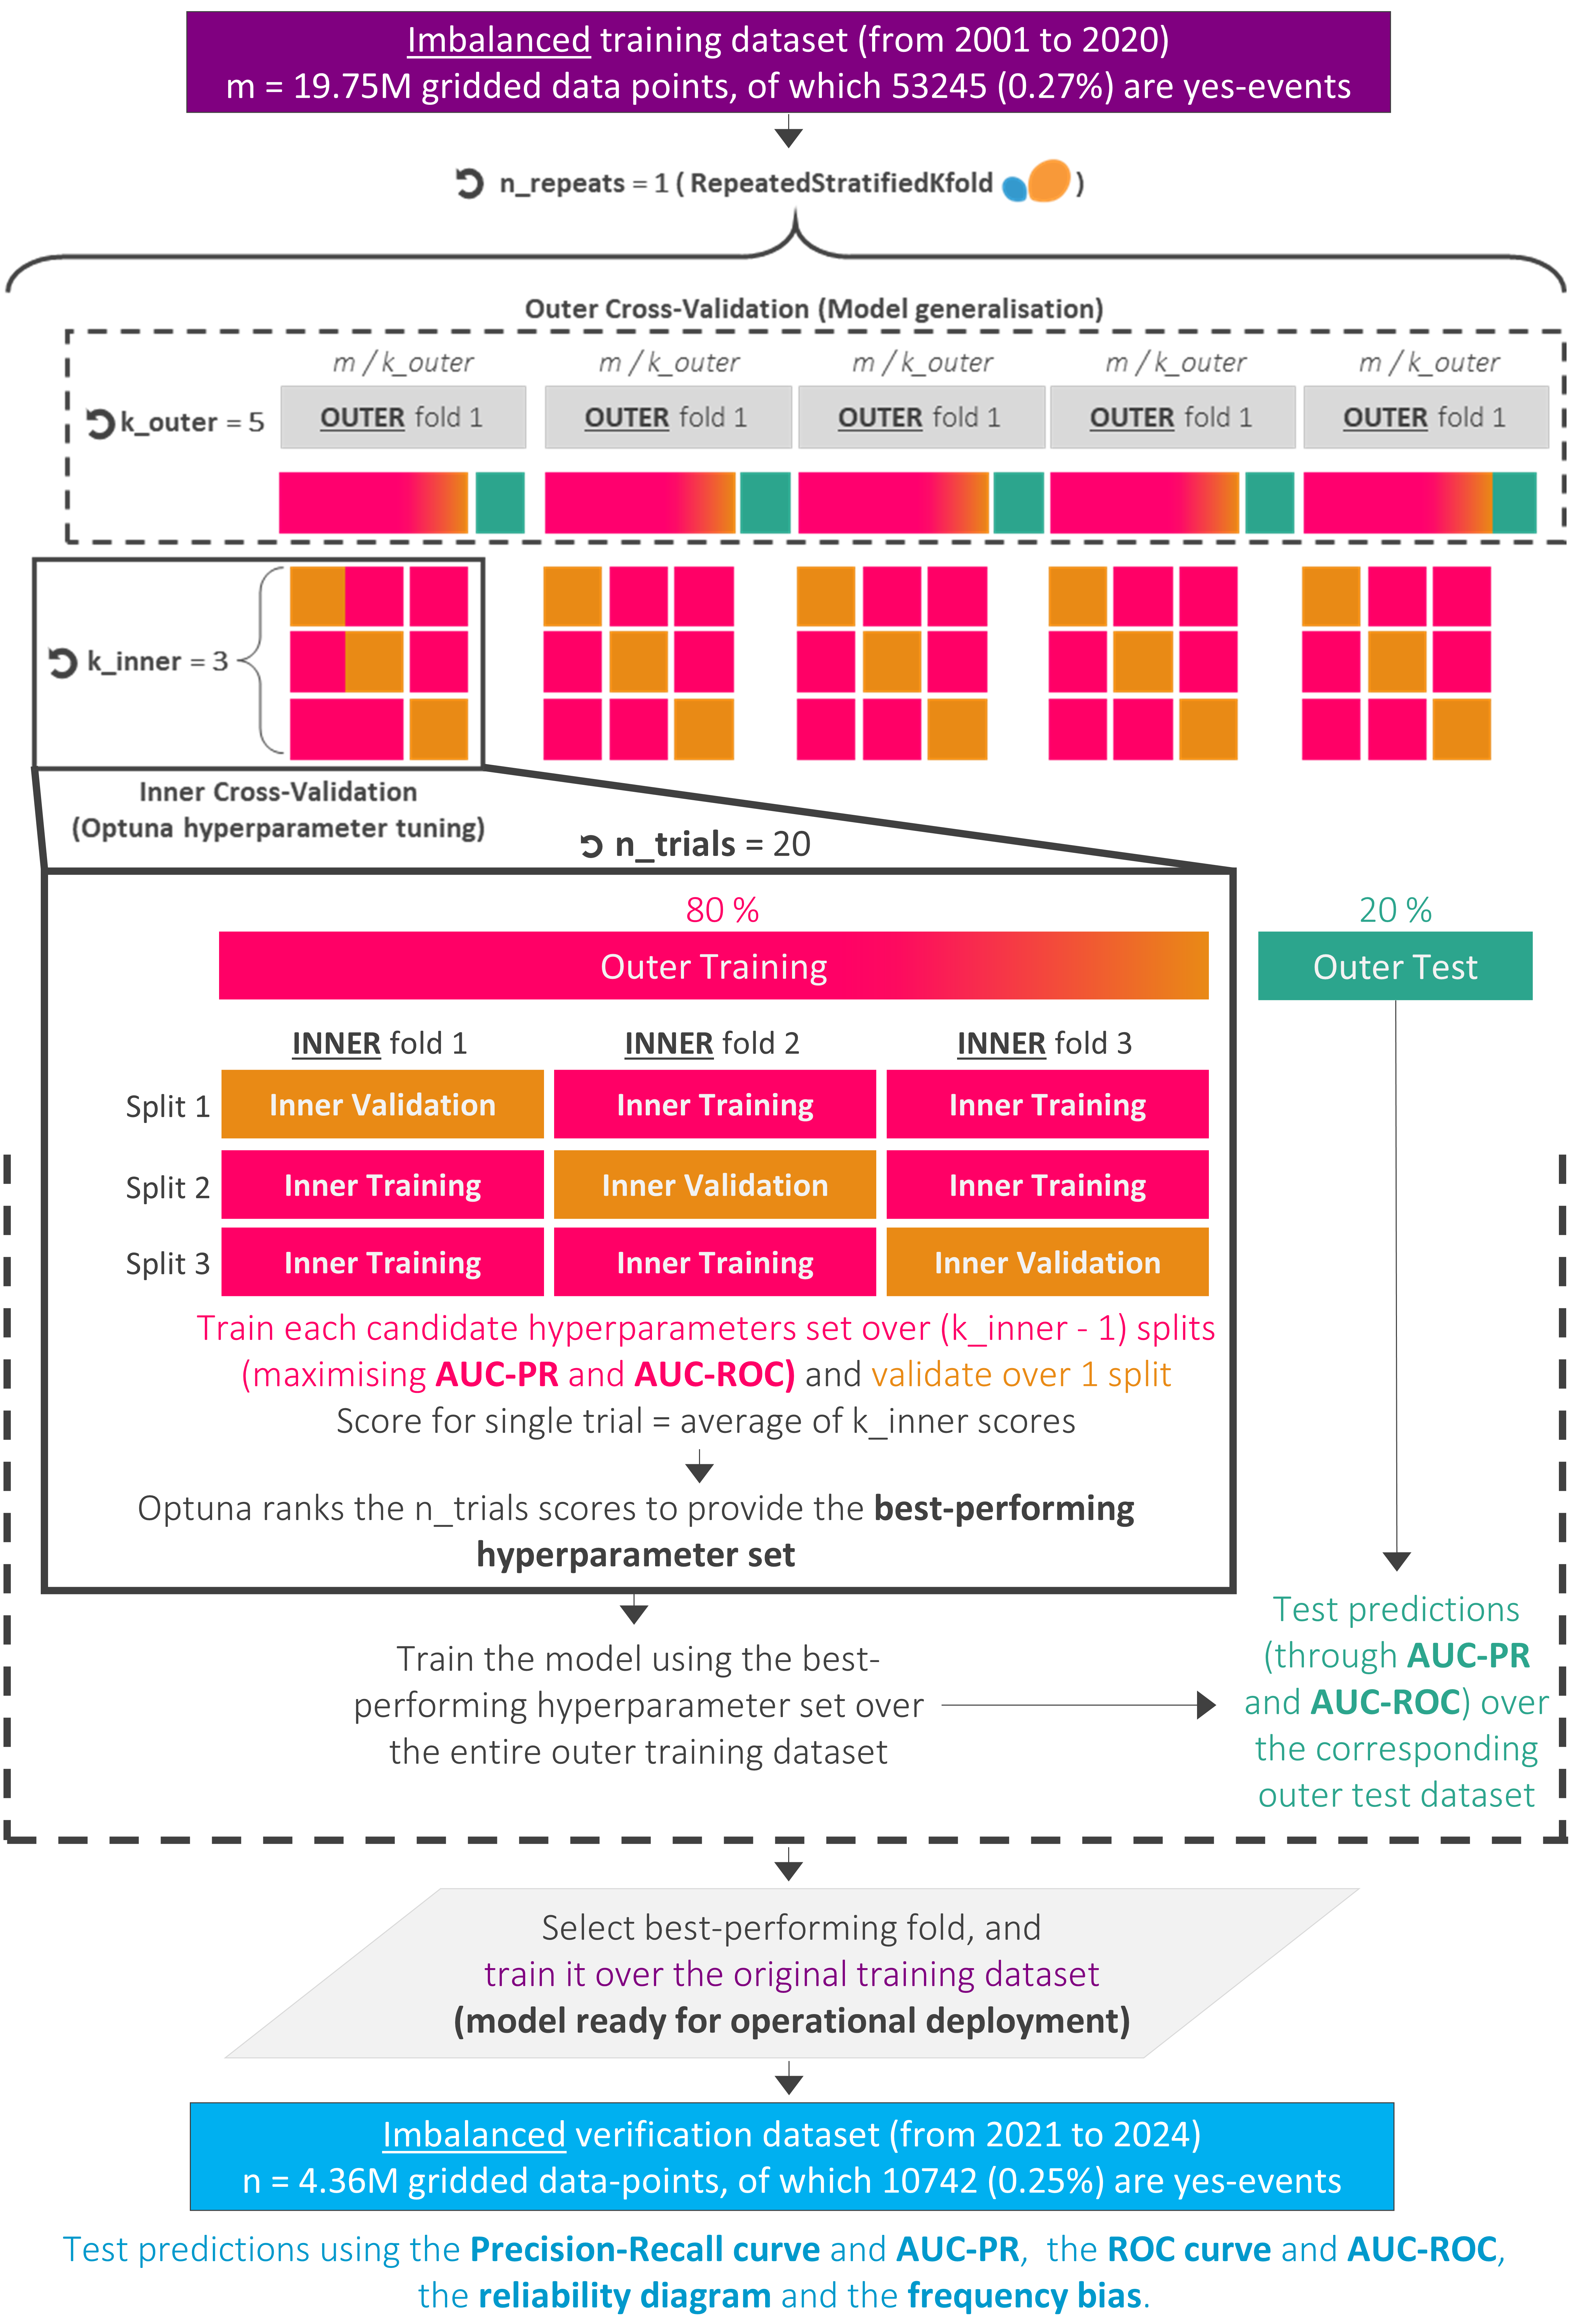
\includegraphics[width=12cm]{figures/cv_optuna.png}
\caption{\textbf{Workflow for the repeated nested cross-validation.} The outer cross-validation loop utilises Scikit-Learn's "RepeatedStratifiedKFold" function to create k\_outer = 5 outer folds (grey blocks) across n\_repeats = 1 iterations. Each \textit{outer fold} maintains the class distribution of the \textit{training dataset}, and it is split into an outer training dataset (80\%, blocks in shades of pink and orange) and an \textit{outer test dataset} (20\%). Within each outer fold, a Bayesian hyperparameter tuning is performed employing the Optuna library through an inner cross-validation procedure over n\_trial = 20 repetitions. Each trial evaluates candidate hyperparameters by training on \textit{inner training folds} and validating on \textit{inner validation folds}, with performance measured as the mean AUC-ROC or AUC-PR. The optimal hyperparameter set, identified by maximising the selected evaluation metric, is used to train the final model on the complete outer training subset. Model performance is assessed on the held-out \textit{outer test fold} using AUC-ROC and AUC-PR. The best-performing fold is retrained on the original \textit{training dataset} for operational deployment. Independent, more extensive verification of the data-driven predictions is performed using the \textit{verification dataset}, considering the Precision-Recall curve and AUC-PR, the ROC curve and AUC-ROC, reliability diagrams, and frequency bias.}
\label{fig:cv_optuna}
\end{figure*}


\subsection{Hyperparameter tuning}

The hyperparameter tuning was conducted using the Python library Optuna \citep{Akiba_2019}. The framework implements a Bayesian optimisation algorithm, primarily utilising the Tree-structured Parzen Estimator (TPE) sampler, which models the relationship between hyperparameters and objective function values to navigate high-dimensional search spaces efficiently. This approach significantly outperforms traditional grid search and random search methods, particularly when computational resources are limited or when the hyperparameter space is complex and continuous. The framework's architecture enables dynamic construction of search spaces where hyperparameters can be conditionally dependent on one another. Optuna's pruning capabilities represent a crucial innovation for computationally intensive tasks, allowing early termination of unpromising trials based on intermediate performance metrics. Moreover, the MedianPruner implementations monitor trial progress and eliminate configurations that are statistically unlikely to surpass previously observed performance, thereby focusing computational resources on promising regions of the hyperparameter space. This feature proves particularly valuable when training deep neural networks or large ensemble models, where individual trial evaluation may require substantial time. Optuna's integration with popular machine learning frameworks such as XGBoost, LightGBM, CatBoost, and TensorFlow handle framework-specific optimisations such as early stopping criteria and validation monitoring, whilst maintaining compatibility with Optuna's pruning mechanisms. Finally, the comprehensive logging and visualisation capabilities facilitate post-hoc analysis of optimisation trajectories, parameter importance assessment, and convergence diagnostics, providing valuable insights into model behaviour and hyperparameter interactions.

The Bayesian optimisation process conducted through Optuna evaluated n\_trial = 20 distinct hyperparameter configurations, with each trial exploring different regions of the search space guided by the Tree-structured Parzen Estimator algorithm.


\subsection{Loss functions}

The training framework implements a dual-strategy approach to address class imbalance through loss function configuration, enabling empirical determination of whether class weighting improves predictive performance for the specific characteristics of flash flood data. 

For balanced datasets or when class imbalance is not a primary concern, the standard \textit{binary cross-entropy (BCE) loss function} is employed without modification. The standard BCE treats the binary classes equally, computing the negative log-likelihood of the predicted probabilities without any weighting mechanism. For tree-based models, the equivalent implementations include \textit{binary:logistic} objective for XGBoost, \textit{binary} objective for LightGBM, and \textit{Logloss} objective for CatBoost. These standard formulations assume that misclassification costs are symmetric between classes and that the training data adequately represents the true class distribution, making them suitable when positive and negative instances occur with comparable frequency.

Due to the severe class imbalance inherent in the problem considered in this thesis, the \textit{weighted binary cross-entropy (W-BCE) loss function} is also considered. It assigns differential importance to minority class instances through an optimisable positive class weight parameter (i.e., the class weights are themselves a hyperparameter optimised with Optuna), within the range [1.0, 10.0]. This weighting mechanism compensates for the scarcity of positive examples by increasing their contribution to the overall loss calculation, thereby preventing the model from converging to a trivial solution that simply predicts the majority class, i.e., it penalises misclassifications of rare flash flood events more heavily than false positives. The implementation manifests differently across frameworks: XGBoost and LightGBM utilise the \textit{scale\_pos\_weight} parameter to directly multiply the loss contribution of positive instances, whilst CatBoost employs the \textit{CrossEntropy loss function} with inherent class weighting capabilities. For neural networks, the Keras implementation applies \textit{class weights during batch gradient computation}, effectively rebalancing the optimisation landscape to ensure adequate representation of rare events.


\subsection{Objective verification framework}

The objective verification framework used in this study is the same as that considered in Chapter ?. Specifically, the reader is referred to Section ? for a detailed description on how to convert point impact reports into gridded fields and what scores use to evaluate the data-driven predictions. 

Two differences can be highlighted between the objective verification framework considered here. In this chapter, only two return periods were considered to define rainfall severity - the 1-year return period and the 50-year return period. The reason for not considering all the thresholds in the development of the data-driven models is that they were correlated. This was established by computing the heat map of the collinearity for all the rainfall thresholds (not shown). In a preliminary analysis to decide which rainfall thresholds to consider, the pair of 1- and 50-year return periods provided the best results. Thus, they were the thresholds kept in the analysis presented here.

The second difference lies in the inclusion of the precision-recall (PR) curve to complement the analysis on the discrimination ability of data-driven predictions provided by ROC curves. PR curves are shown to be more suitable for verifying data-driven outputs generated with imbalanced training datasets. In meteorology, PR curves are better known as \textit{Performance Diagrams}, and are primarily used for deterministic predictions. A detailed description of the PR curves and their comparison with ROC curves can be found in Section ?.

Finally, it is worth noting that 99\% confidence intervals were computed via bootstrapping with replacement over 1000 repetitions for all scores. However, the confidence intervals were so small that they were not included in the figures presented in the following section.


\subsection{Physical interpretation of the data-driven model outputs: Shapley values}

Shapley values, derived from cooperative game theory, have emerged as a powerful technique for interpreting complex data-driven models by quantifying the contribution of each input feature to individual predictions \citep{Rozemberczki_2022}. Shapley values decompose a model's prediction into additive contributions from each predictor variable, revealing how each model feature - in this case, rainfall, antecedent soil moisture, orography slope, and vegetation coverage - combine to produce the final prediction - i.e., areas at risk of flash floods. This decomposition provides crucial physical insights into the decision-making process of the data-driven model. In this way, the model becomes \textit{interpretable} because it is possible to assess which variable yields the most importance in defining a prediction and how a model feature modulates the impact of another one. Moreover, it is possible to diagnose potential issues where the model may be relying on spurious correlations. 


\section{Results}

\subsection{Model training}

The hyperparameter optimisation history plot (Figure \ref{fig:optuna_history}) shows the overall good performance of the Optuna library in identifying quickly (within the first 10 trials, orange lines) and with relatively small variations (grey lines) the sets of hyperparameters that maximise the chosen evaluation metrics (AUC-ROC and AUC-PR). Performance remains fairly consistent between different outer folds (lines in shades of grey and orange). The optimisation histories for AUC-ROC (Figure \ref{fig:optuna_history}a-l) and AUC-PR (Figure \ref{fig:optuna_history}m-x) are very similar, with plots for loss functions specific for imbalanced datasets (Figure \ref{fig:optuna_history}g-l and s-x) showing more variability, but in general better overall performance, than those for more general loss functions (Figure \ref{fig:optuna_history}a-f and m-r). 

%f
\begin{figure*}[t]
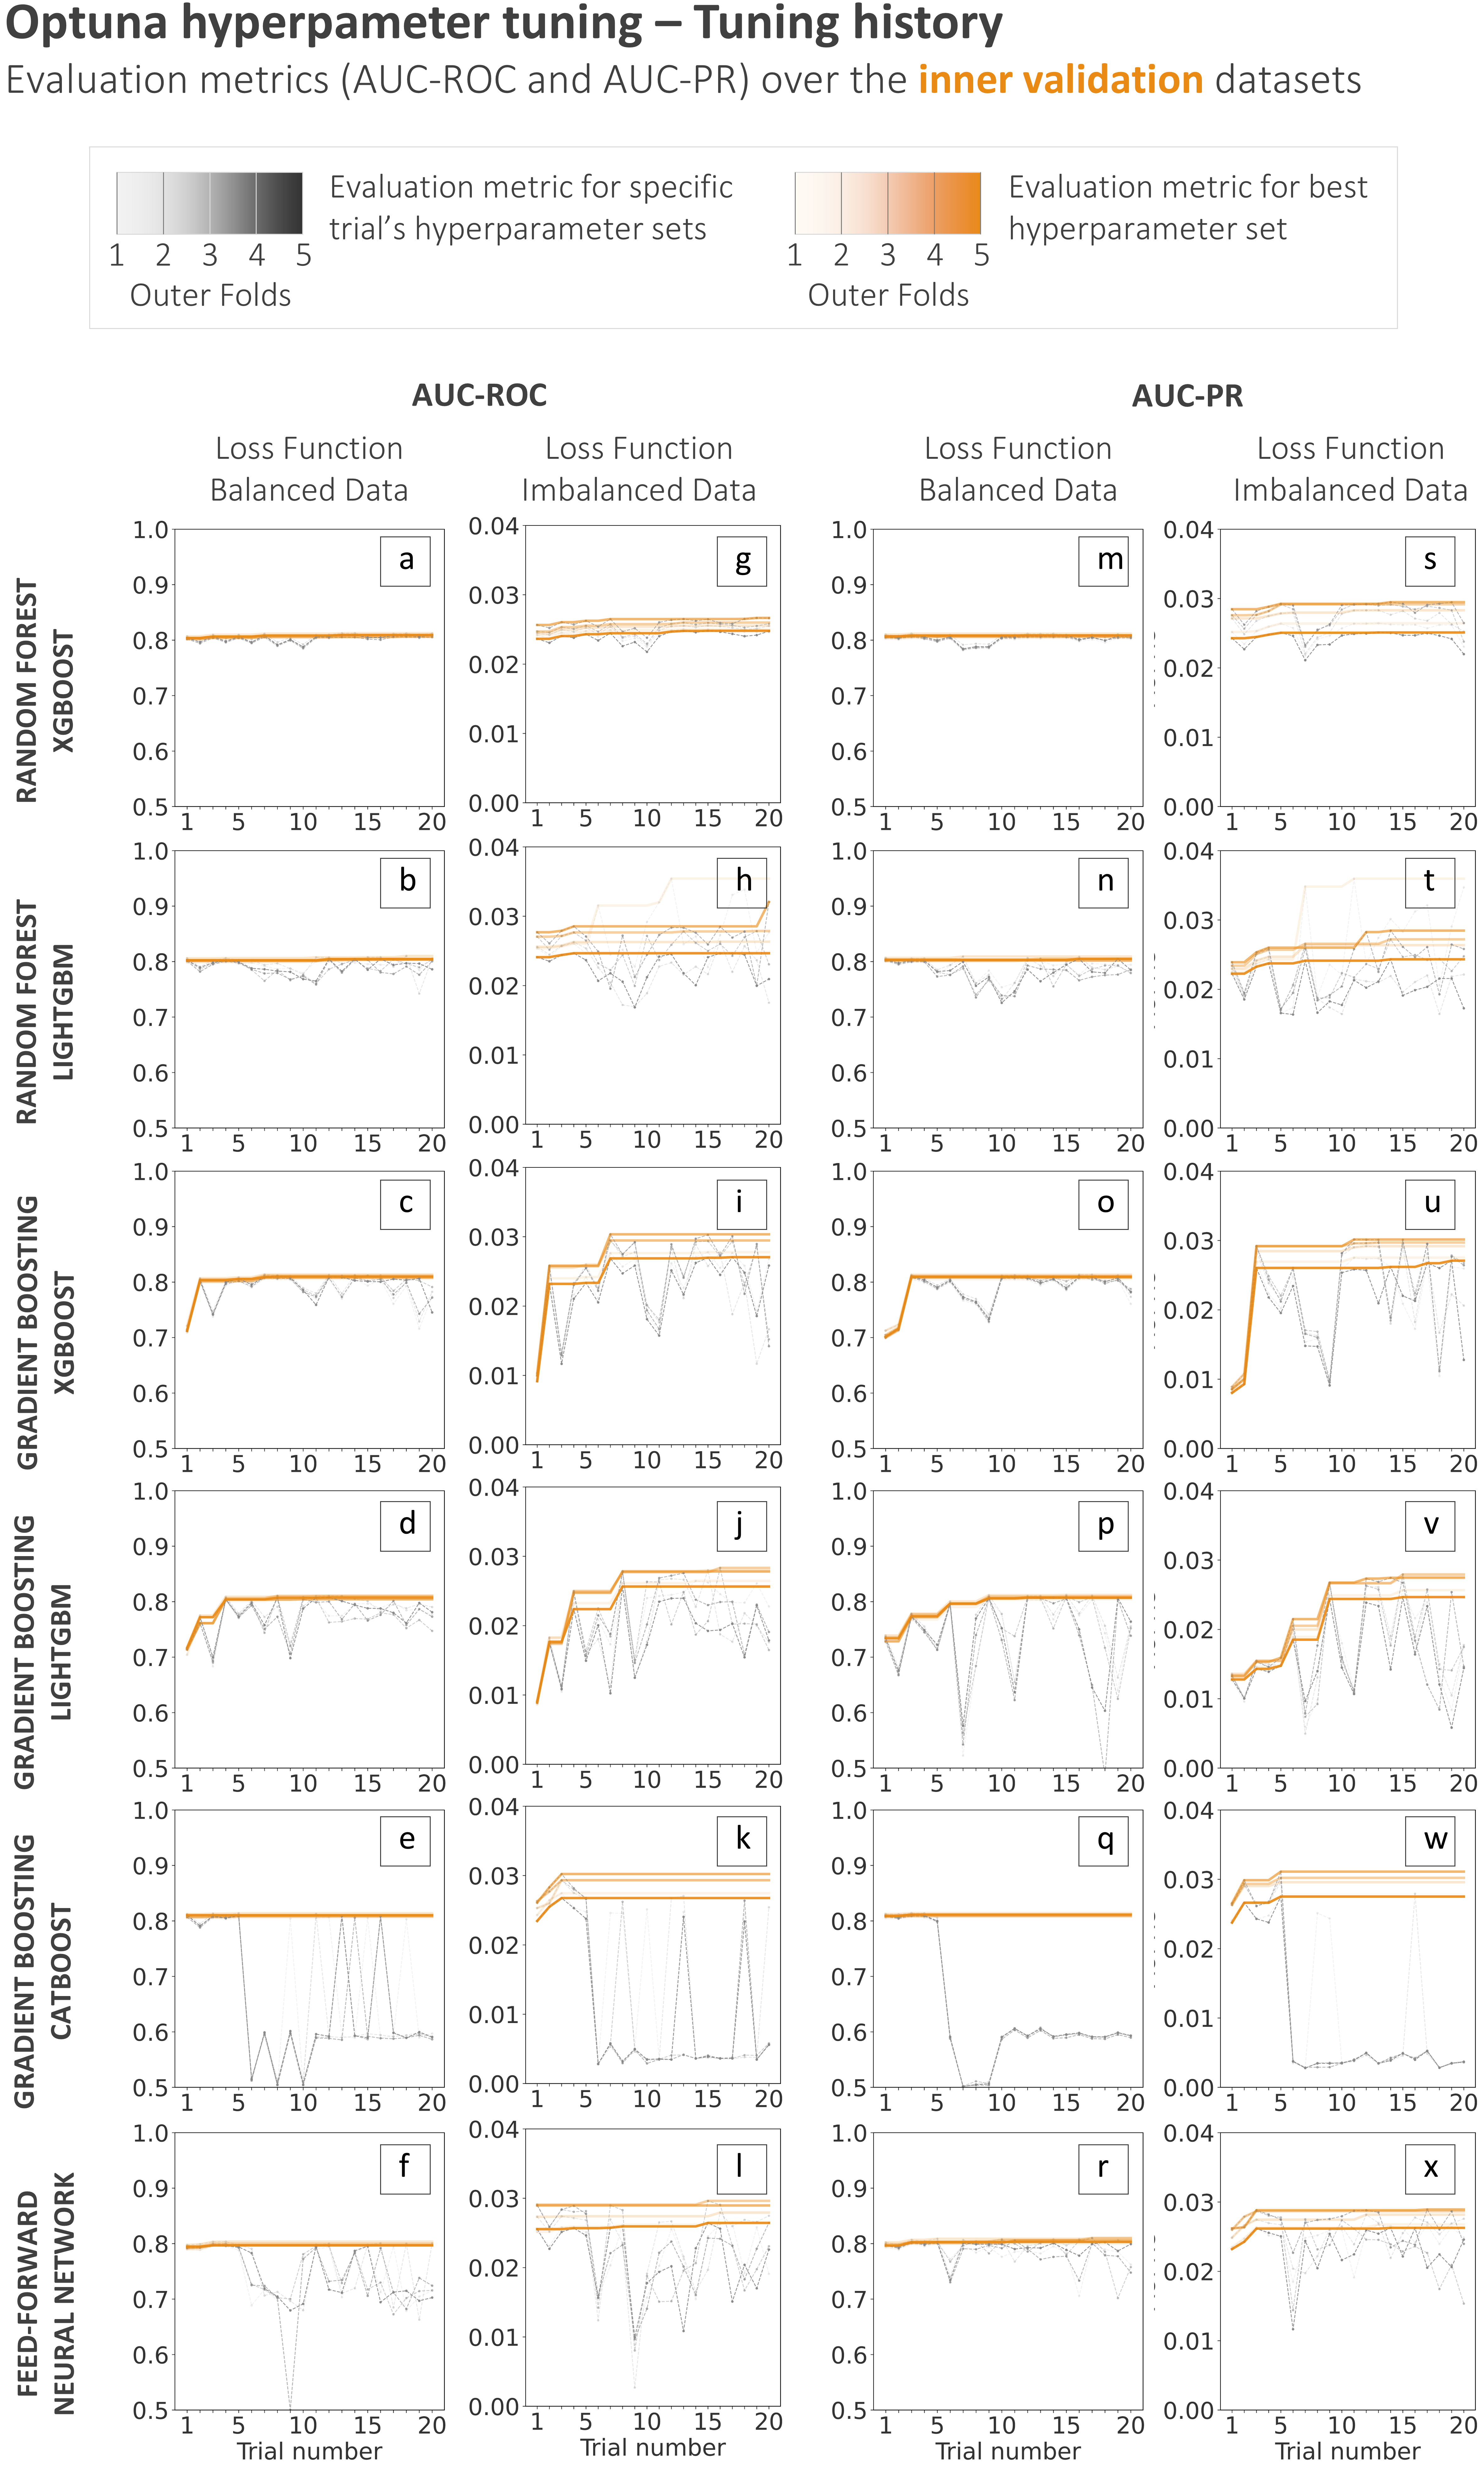
\includegraphics[width=12cm]{figures/optuna_history.png}
\caption{\textbf{Optuna's hyperparameter optimisation history.} Evolution of the two evaluation metrics (AUC-ROC, panels (a) to (l) - and AUC-PR, panels (m) to (x)) maximised during the 20 trials run over the \textit{inner validation folds} to tune the hyperparameters of six data-driven models (from top to bottom): random forest XGBoost, random forest LightGBM, gradient boosting XGBoost, gradient boosting LightGBM, gradient boosting CatBoost, and feed-forward neural network. The lines in shades of grey indicate individual trial performances, whilst lines in shades of orange highlight the best-performing hyperparameter set, identified by Optuna's Bayesian optimisation process. The shades of grey and orange represent the values of the evaluation metrics for each outer fold (lightest shade for the first outer fold and darkest for the latest). Panels (a) to (f) and (m) to (r) represents the results obtained using the standard binary cross-entropy loss functions - mostly used for balanced datasets - whilst panels (g) to (l) and (s) to (x) present the outcomes obtained with the weighted loss functions (specifically configured for imbalanced data).}
\label{fig:optuna_history}
\end{figure*}

The training times show substantial computational differences across model architectures (Figure \ref{fig:optuna_training_time}). Decision-tree-based implementations (except for CatBoost) demonstrate more efficient training times. On average, the training time per outer fold remains between 75 and 100 seconds, with peaks that do not exceed 500 seconds. CatBoost's training times are around 500 seconds per outer fold, with peaks reaching 2000 seconds. The feed-forward neural network exhibits the longest training times among all models, with an average training time of around 2000 seconds and peaks ranging from 4000 to 6000 seconds. These times indicate that it requires ~20 minutes per outer fold to optimise hyperparameters and train the decision-tree-based models (except for CatBoost), compared to ~2.5 and ~8 hours per outer fold, respectively, for CatBoost and the feed-forward neural network. The choice of loss function and evaluation metric shows minimal impact on training duration across all architectures.

%f
\begin{figure*}[t]
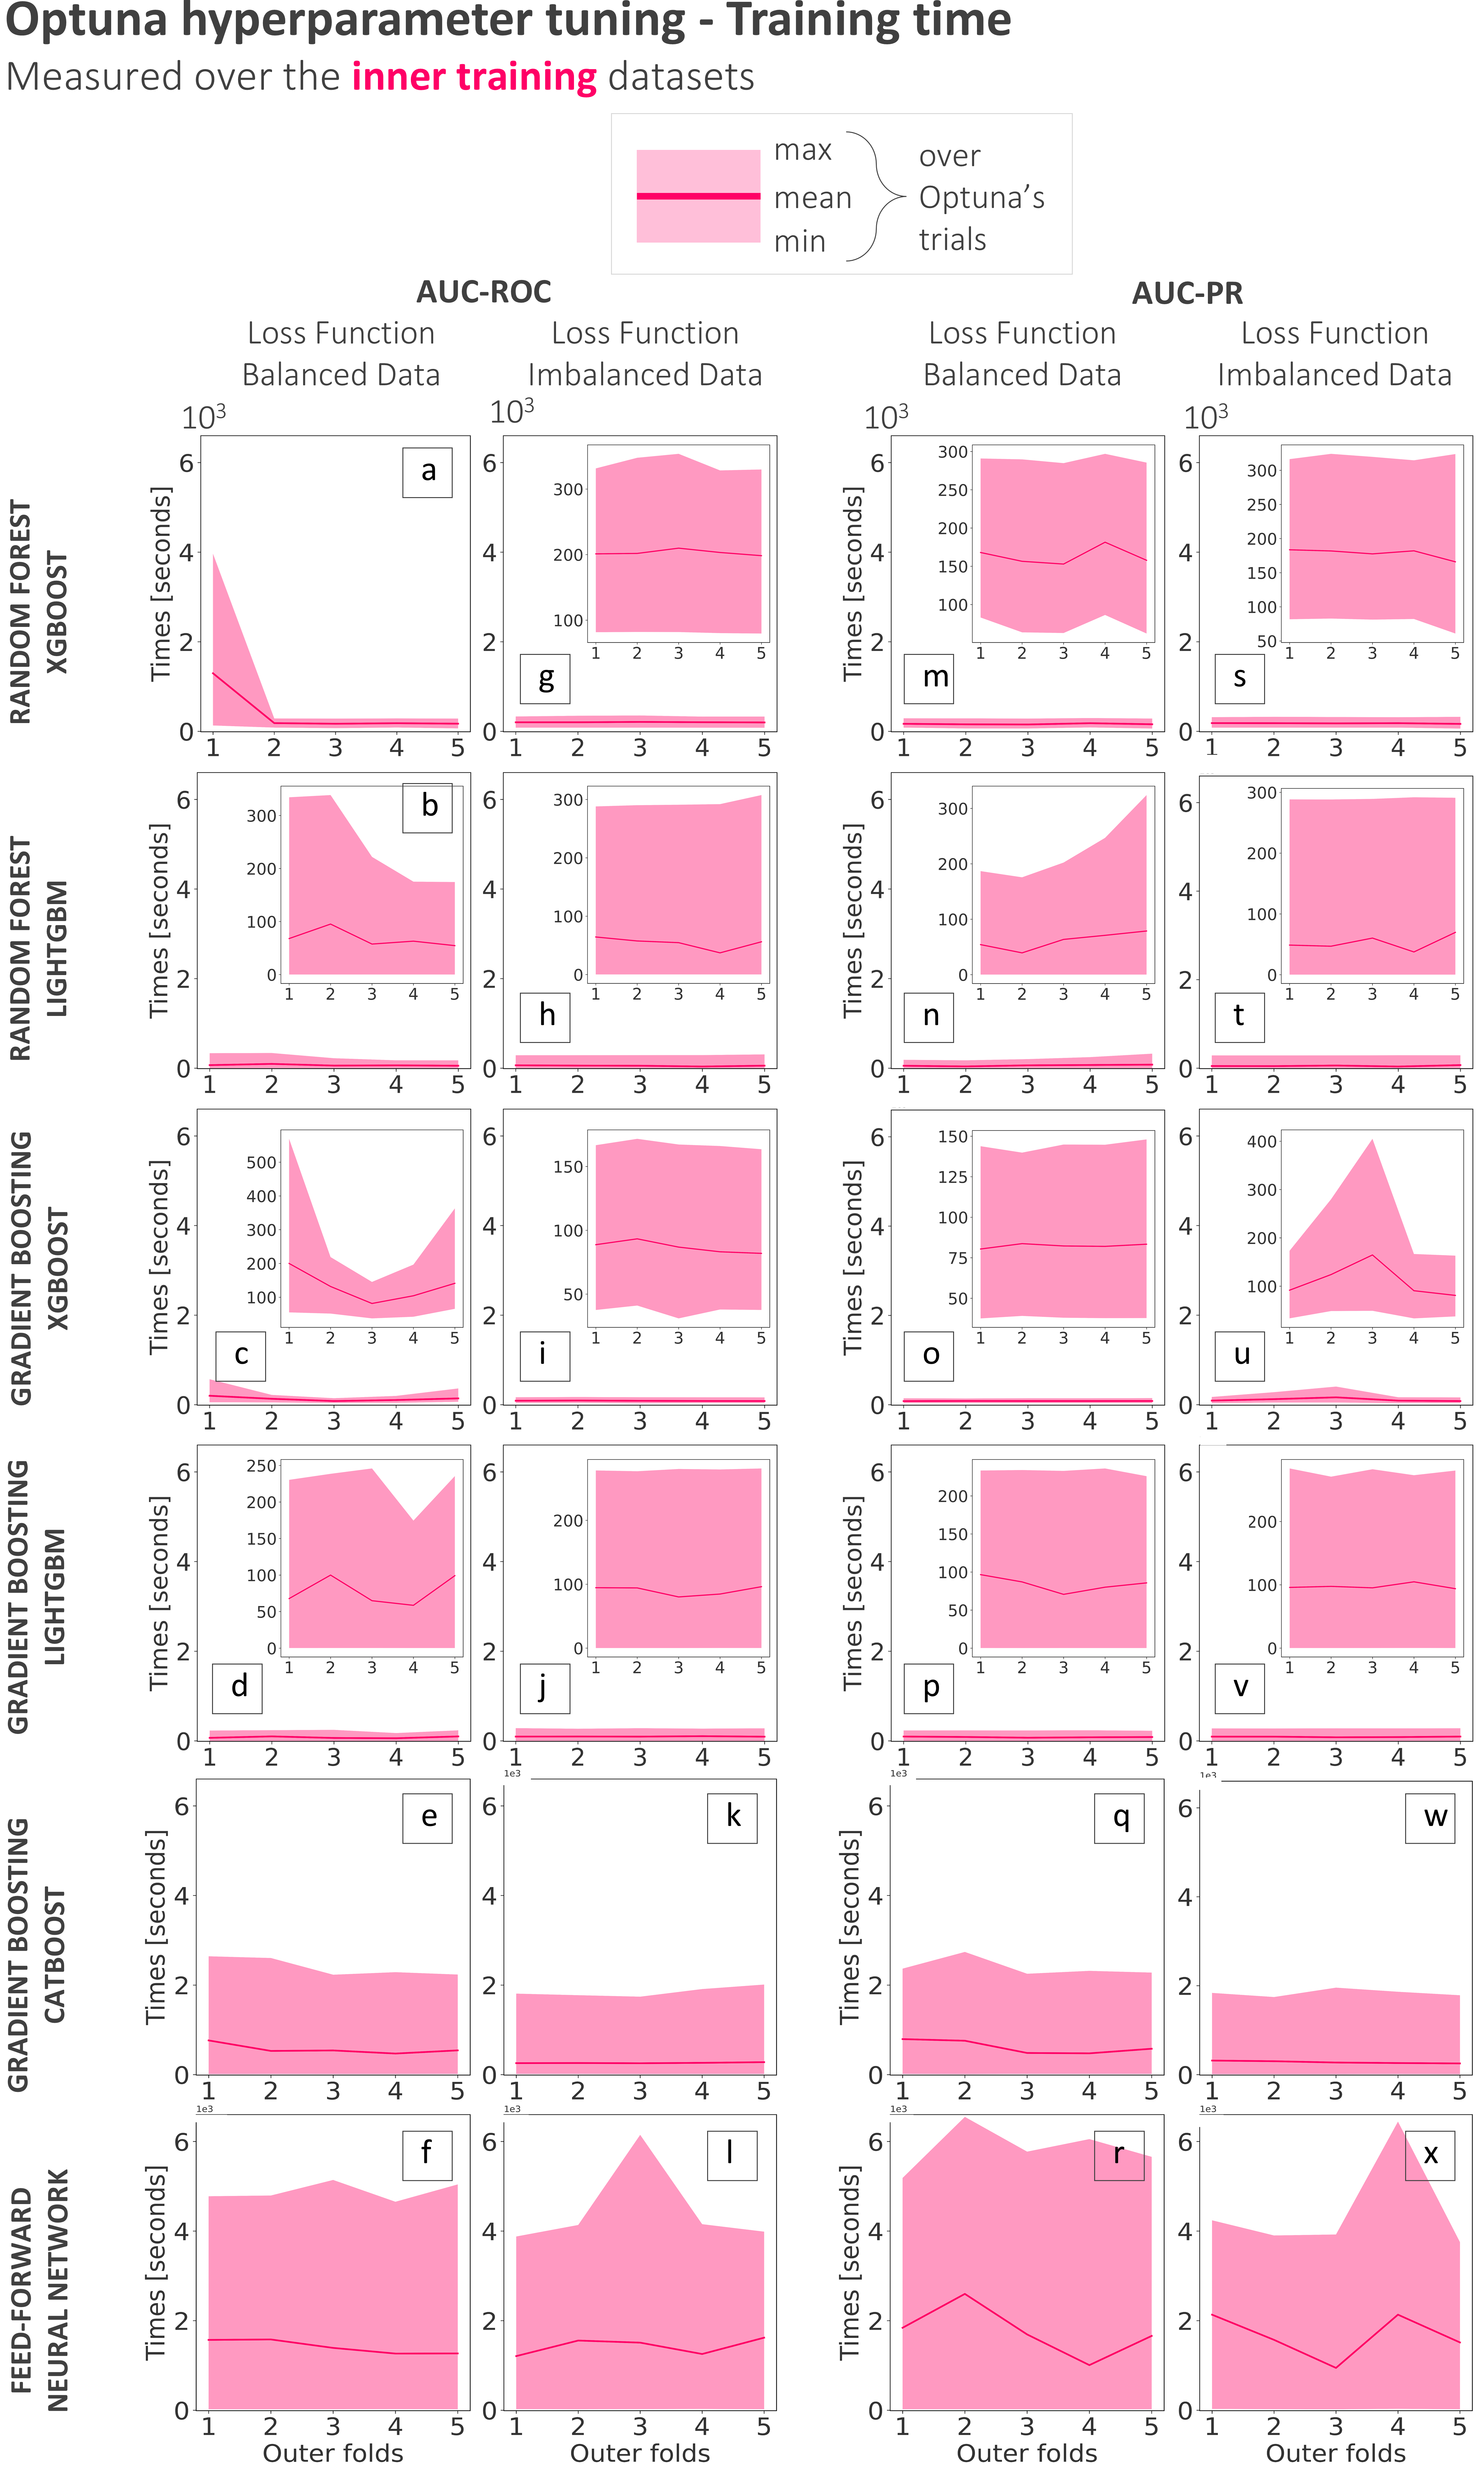
\includegraphics[width=12cm]{figures/optuna_time_training.png}
\caption{\textbf{Optuna's training time.} Evolution of training times (in seconds) for each k\_outer=5 outer folds across the n\_trials = 20 trials run over the \textit{inner training folds} (the solid line represents the mean while the shaded area represents the minimum and maximum values). The training times for six data-driven models (from top to bottom) are shown: random forest XGBoost, random forest LightGBM, gradient boosting XGBoost, gradient boosting LightGBM, gradient boosting CatBoost, and feed-forward neural network. Training times are shown for both evaluation metrics (AUC-ROC - panels (a) to (l) - and AUC-PR - panels (m) to (x)) and loss function configurations (balanced and imbalanced datasets). Inset plots provide magnified views where appropriate.}
\label{fig:optuna_time_training}
\end{figure*}

The close values for both evaluation metrics (AUC-ROC and AUC-PR) estimated over the \textit{inner validation folds} and the \textit{outer test folds} show the robustness of the nested cross-validation framework in mitigating overfitting during hyperparameter optimisation  (Figure \ref{fig:optuna_evaluation_metrics}). The fact that outer test performance remains generally bounded or close to the performance ranges estimated over the inner validation folds demonstrates that Optuna's Bayesian optimisation successfully identified hyperparameter configurations with robust generalisation capabilities to previously unseen data. The comparative analysis reveals minimal divergence between models trained with standard binary cross-entropy and those employing weighted loss functions (formulated specifically for class-imbalanced datasets). This observation holds for both evaluation metrics. Across the evaluated models, performance metrics demonstrate remarkable consistency, with the notable exception of CatBoost. Specifically, mean AUC-ROC values cluster between 0.7 and 0.8, whilst CatBoost exhibits inferior performance with values between 0.6 and 0.7. Similarly, mean AUC-PR values range from 0.02 to 0.03 across most models, with CatBoost again demonstrating diminished performance with values between 0.01 and 0.02. For both metrics, random forest implementations exhibit the narrowest bands, followed by gradient boosting implementations (except for CatBoost, which displays the widest bands among all models) and the feed-forward neural network. The wider bands for CatBoost exhibit greater sensitivity to hyperparameter choices and require more careful tuning to achieve optimal results. Random forest implementations exhibit the most constrained performance bands, indicating robust hyperparameter spaces that yield consistent results across outer folds. Gradient boosting implementations (except for CatBoost) and the feed-forward neural network demonstrate intermediate variability. CatBoost exhibits the broadest performance bands amongst all evaluated models, suggesting that CatBoost's hyperparameter space possesses heightened sensitivity, necessitating more meticulous optimisation procedures to achieve competitive performance levels.

%f
\begin{figure*}[t]
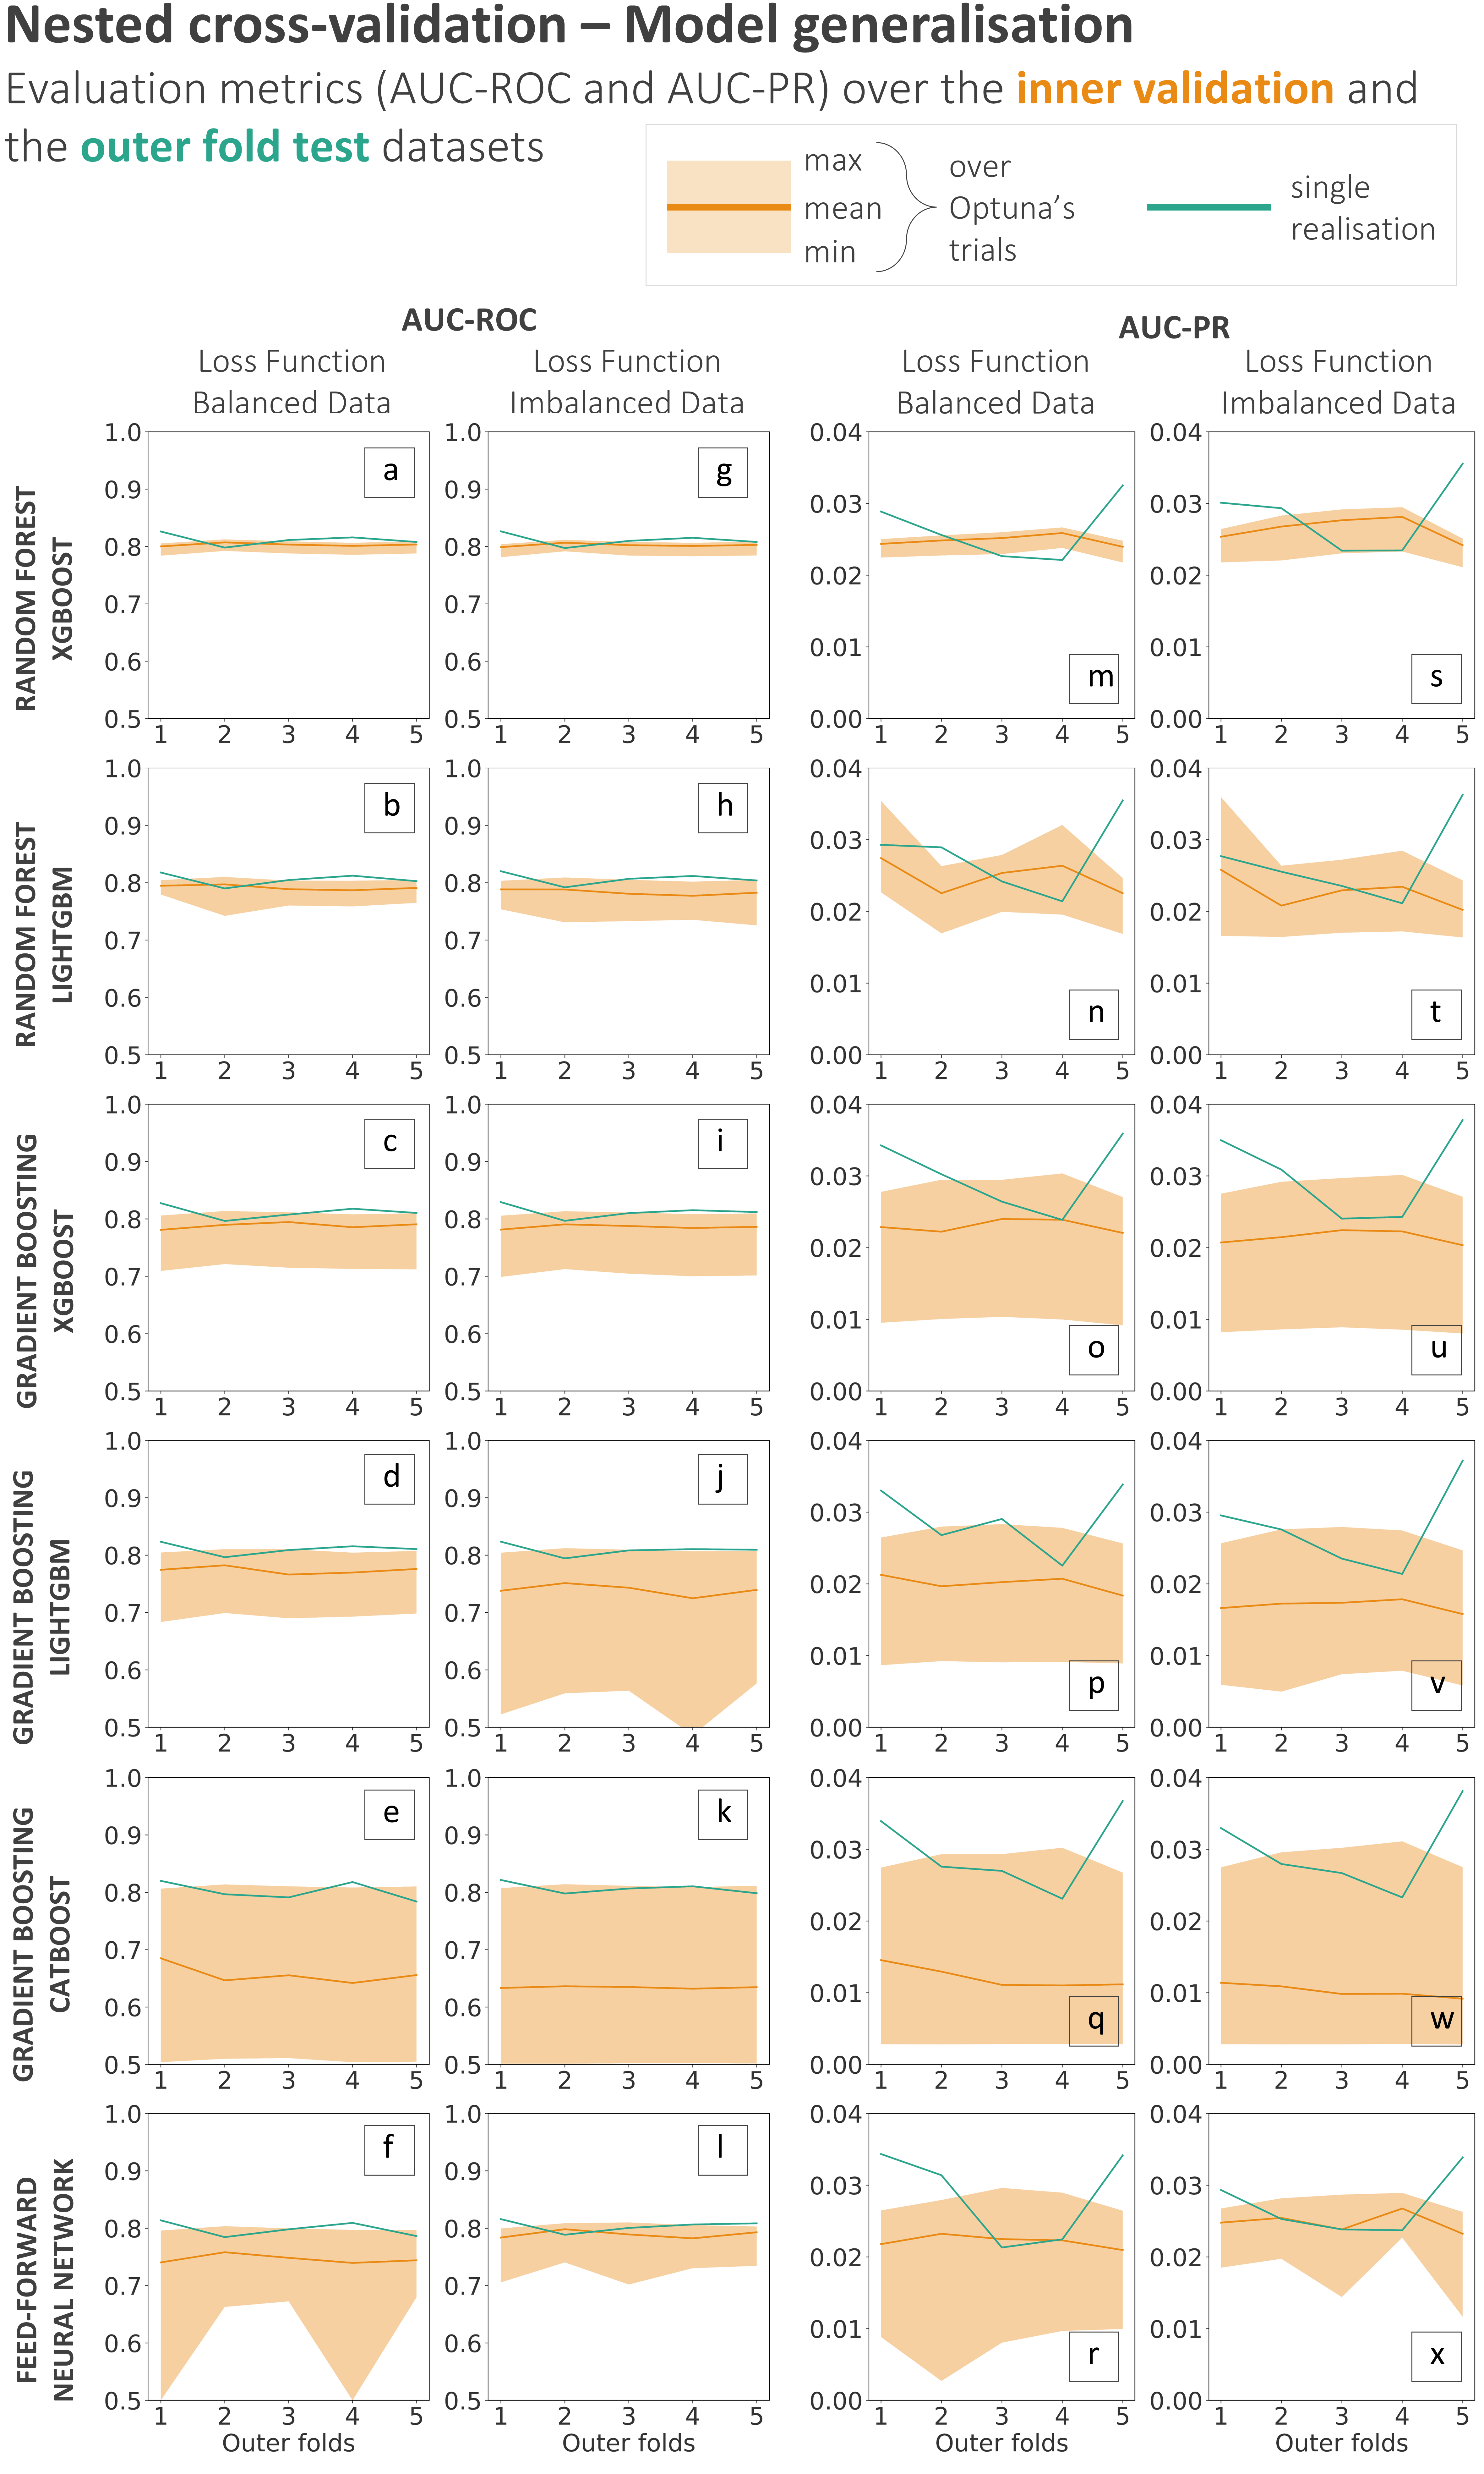
\includegraphics[width=12cm]{figures/optuna_evaluation_metrics.png}
\caption{\textbf{Model generalisation from nested cross-validation} Values of the two evaluation metrics (AUC-ROC, panels (a) to (l) - and AUC-PR, panels (m) to (x)) across the 20 trials run over the \textit{inner validation folds} (the solid line represents the mean while the shaded area represents the minimum and maximum values) and the \textit{outer test fold} (the solid line correspond to the single realisation per outer fold). Panels (a) to (f) and (m) to (r) represents the results obtained using the standard binary cross-entropy loss functions - mostly used for balanced datasets - whilst panels (g) to (l) and (s) to (x) present the outcomes obtained with the weighted loss functions (specifically configured for imbalanced data).}
\label{fig:optuna_evaluation_metrics}
\end{figure*}


\subsubsection{Hyperparameter importance}

The hyperparameter importance analysis for XGBoost and LightGBM gradient boosting implementations reveals that maximum depth and learning rate consistently emerge as the most influential parameters. This aspect suggests that optimal performance depends fundamentally on striking a balance between model complexity and convergence dynamics. Maximum depth controls the model's capacity to capture complex hydro-meteorological interactions, whilst learning rate determines the magnitude of iterative corrections, requiring careful calibration to preserve gradient signals from rare positive events. LightGBM demonstrates additional sensitivity to the number of estimators due to its leaf-wise tree construction, producing more informative individual trees that necessitate precise ensemble size optimisation. In contrast, XGBoost's level-wise approach generates simpler trees that plateau predictably, reducing the criticality of this parameter. Notably, the positive class weight parameter exhibits a generally lower influence across both implementations, suggesting that structural parameters governing tree complexity and learning dynamics exert a greater impact on minority class detection than explicit re-weighting strategies. Thus, this emphasises the primacy of architectural optimisation over class balancing approaches. CatBoost exhibits considerable variability in the hyperparameters that most strongly influence model performance, with this variability dependent on both the chosen evaluation metric and the loss function configuration. When optimising for AUC-ROC, a set of parameters proves critical (e.g. depth and learning rate), yet these same parameters have minimal impact when considering AUC-PR. Furthermore, the implementation of weighted loss functions fundamentally alters the previously seen importance rankings, creating distinct optimisation priorities for balanced versus imbalanced scenarios. Unlike XGBoost and LightGBM, where maximum depth and learning rate consistently dominate, CatBoost lacks such universal governing parameters. The absence of consistent parameter hierarchies suggests that CatBoost's distinctive algorithmic approach generates a more complex hyperparameter space. 

%f
\begin{figure*}[t]
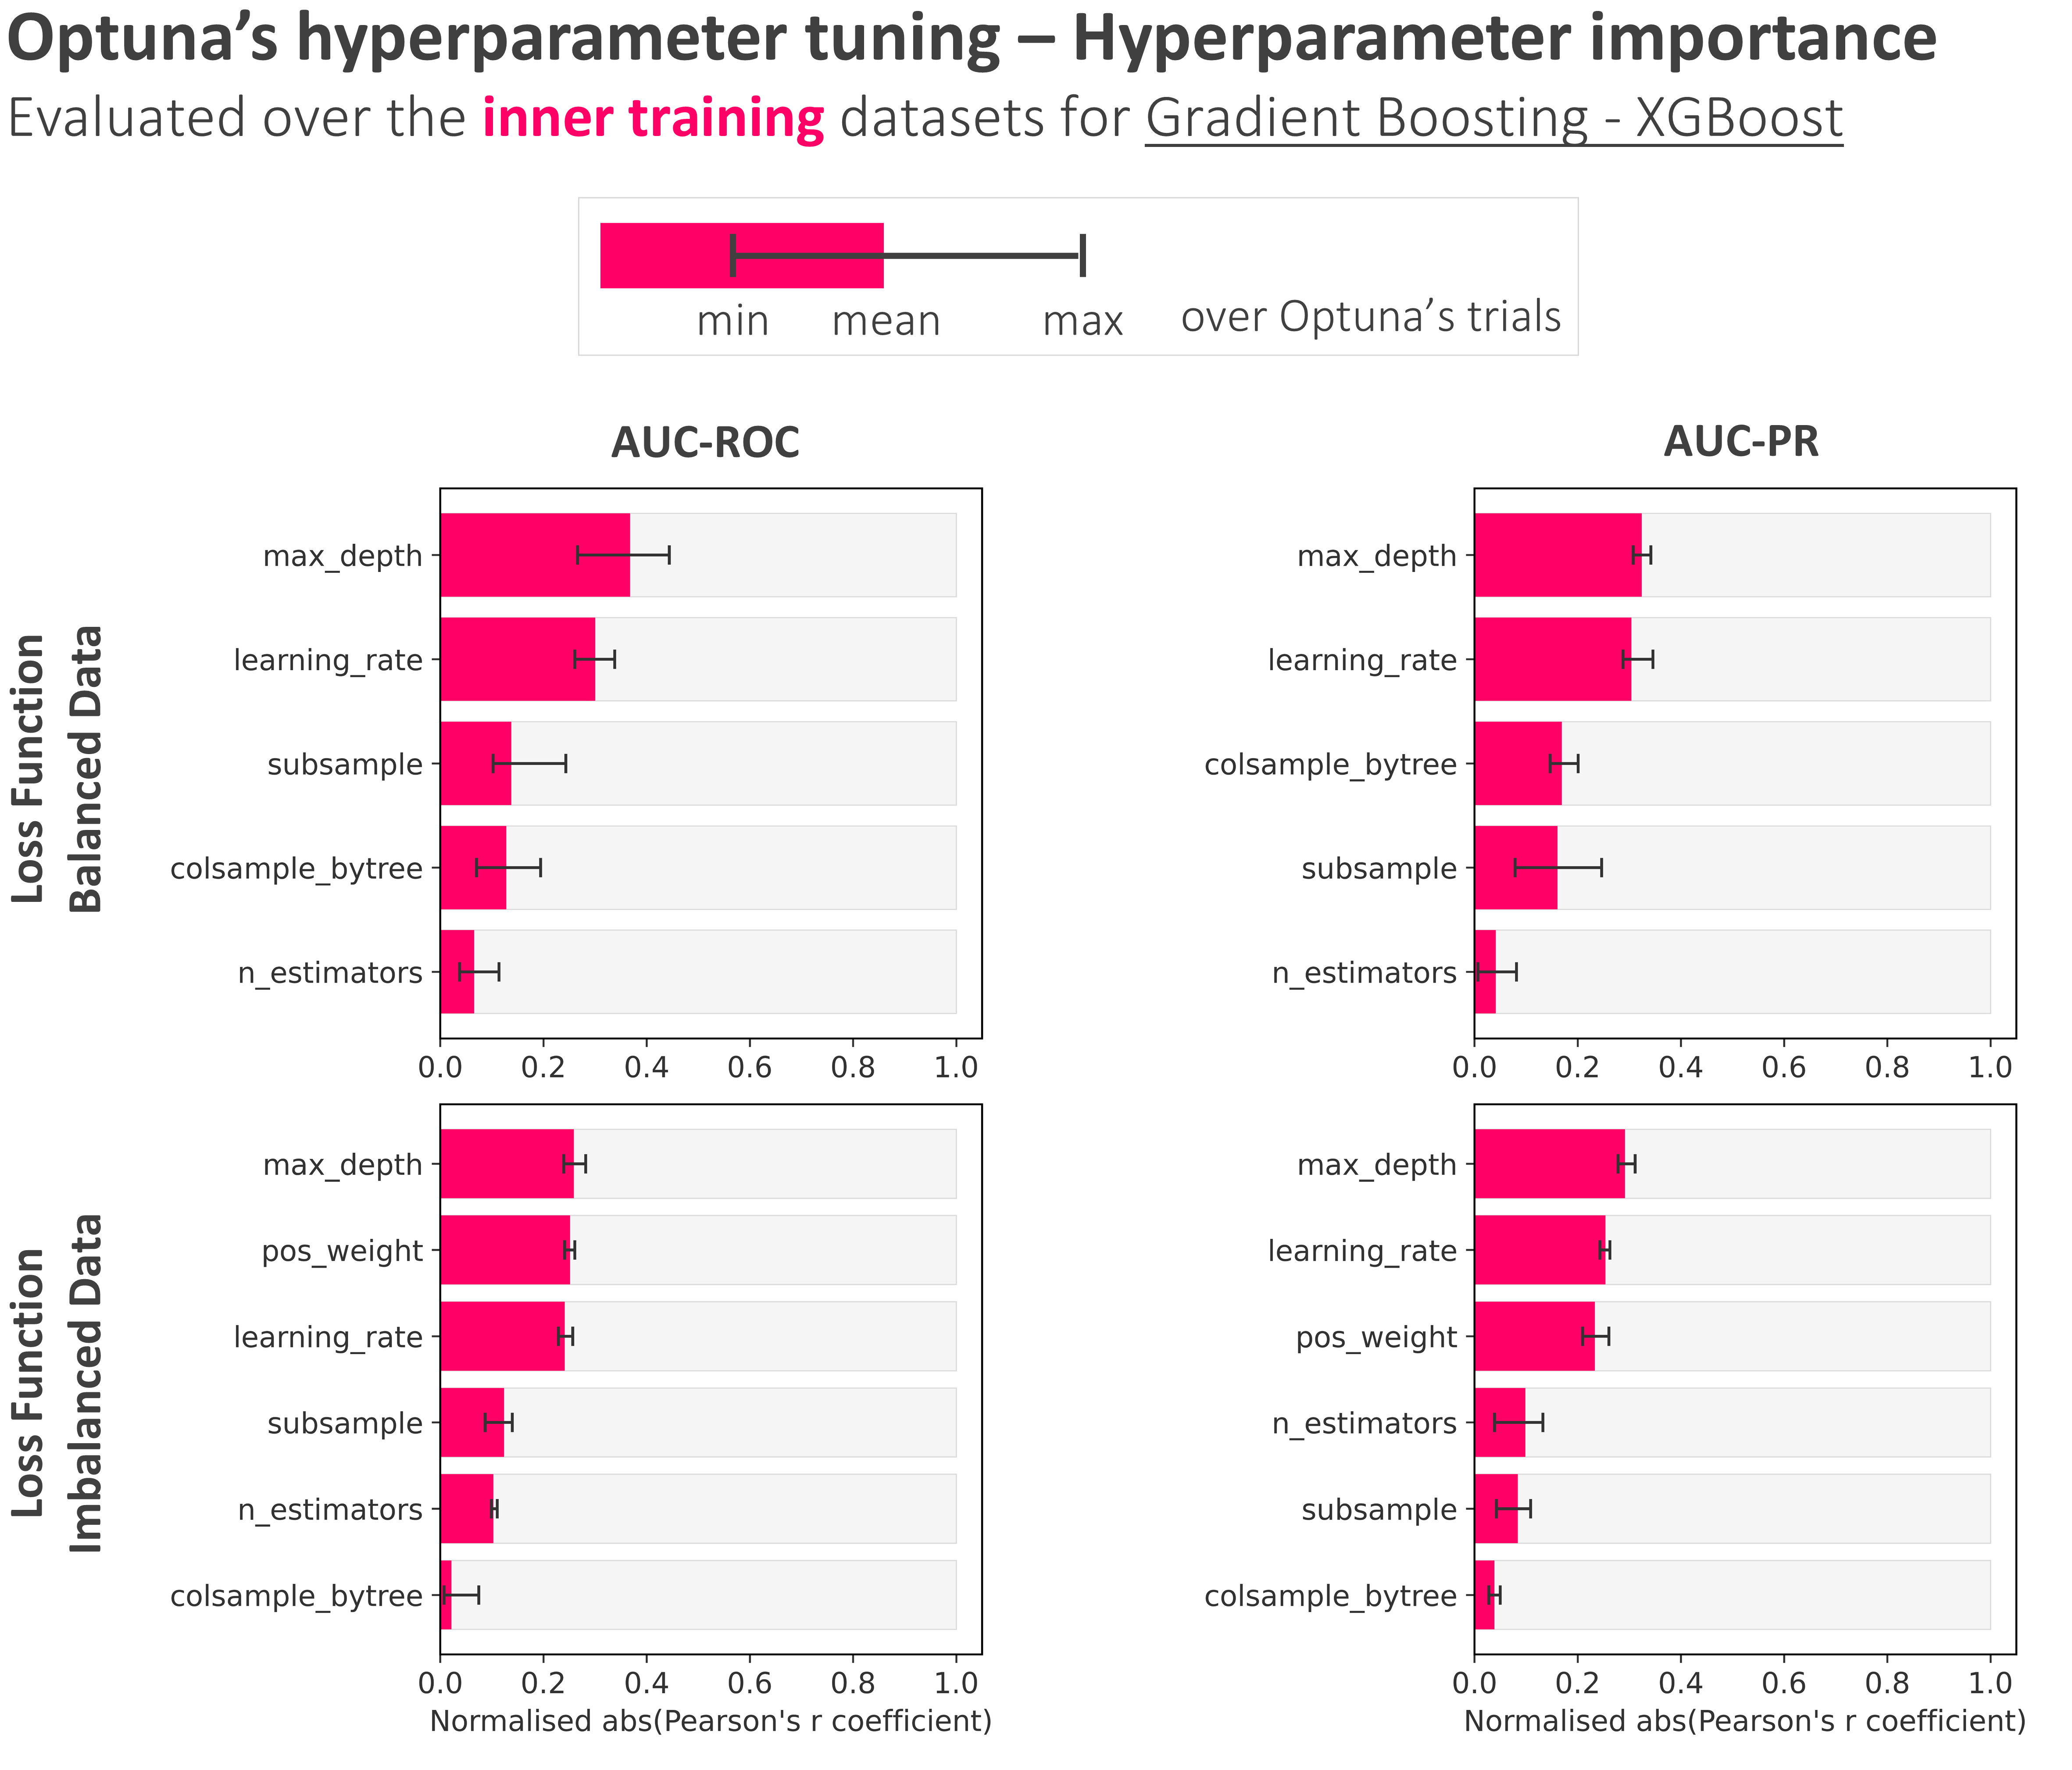
\includegraphics[width=12cm]{figures/optuna_parameters_importance_gradient_boosting_xgboost.png}
\caption{\textbf{Optuna's hyperparameter importance for the XGBoost implementation of gradient boosting.} Normalised absolute Pearson's correlation coefficients obtained for the n\_trials = 20 trials run over the \textit{inner training folds} (bars represent mean values, whilst error bars show the minimum and maximum values across the Optuna trials). Feature importance is shown for models trained with loss functions for balanced datasets and specific for imbalanced datasets, and for both evaluation metrics (AUC-ROC and AUC-PR).}
\label{fig:optuna_parameters_importance_gradient_boosting_xgboost}
\end{figure*}

%f
\begin{figure*}[t]
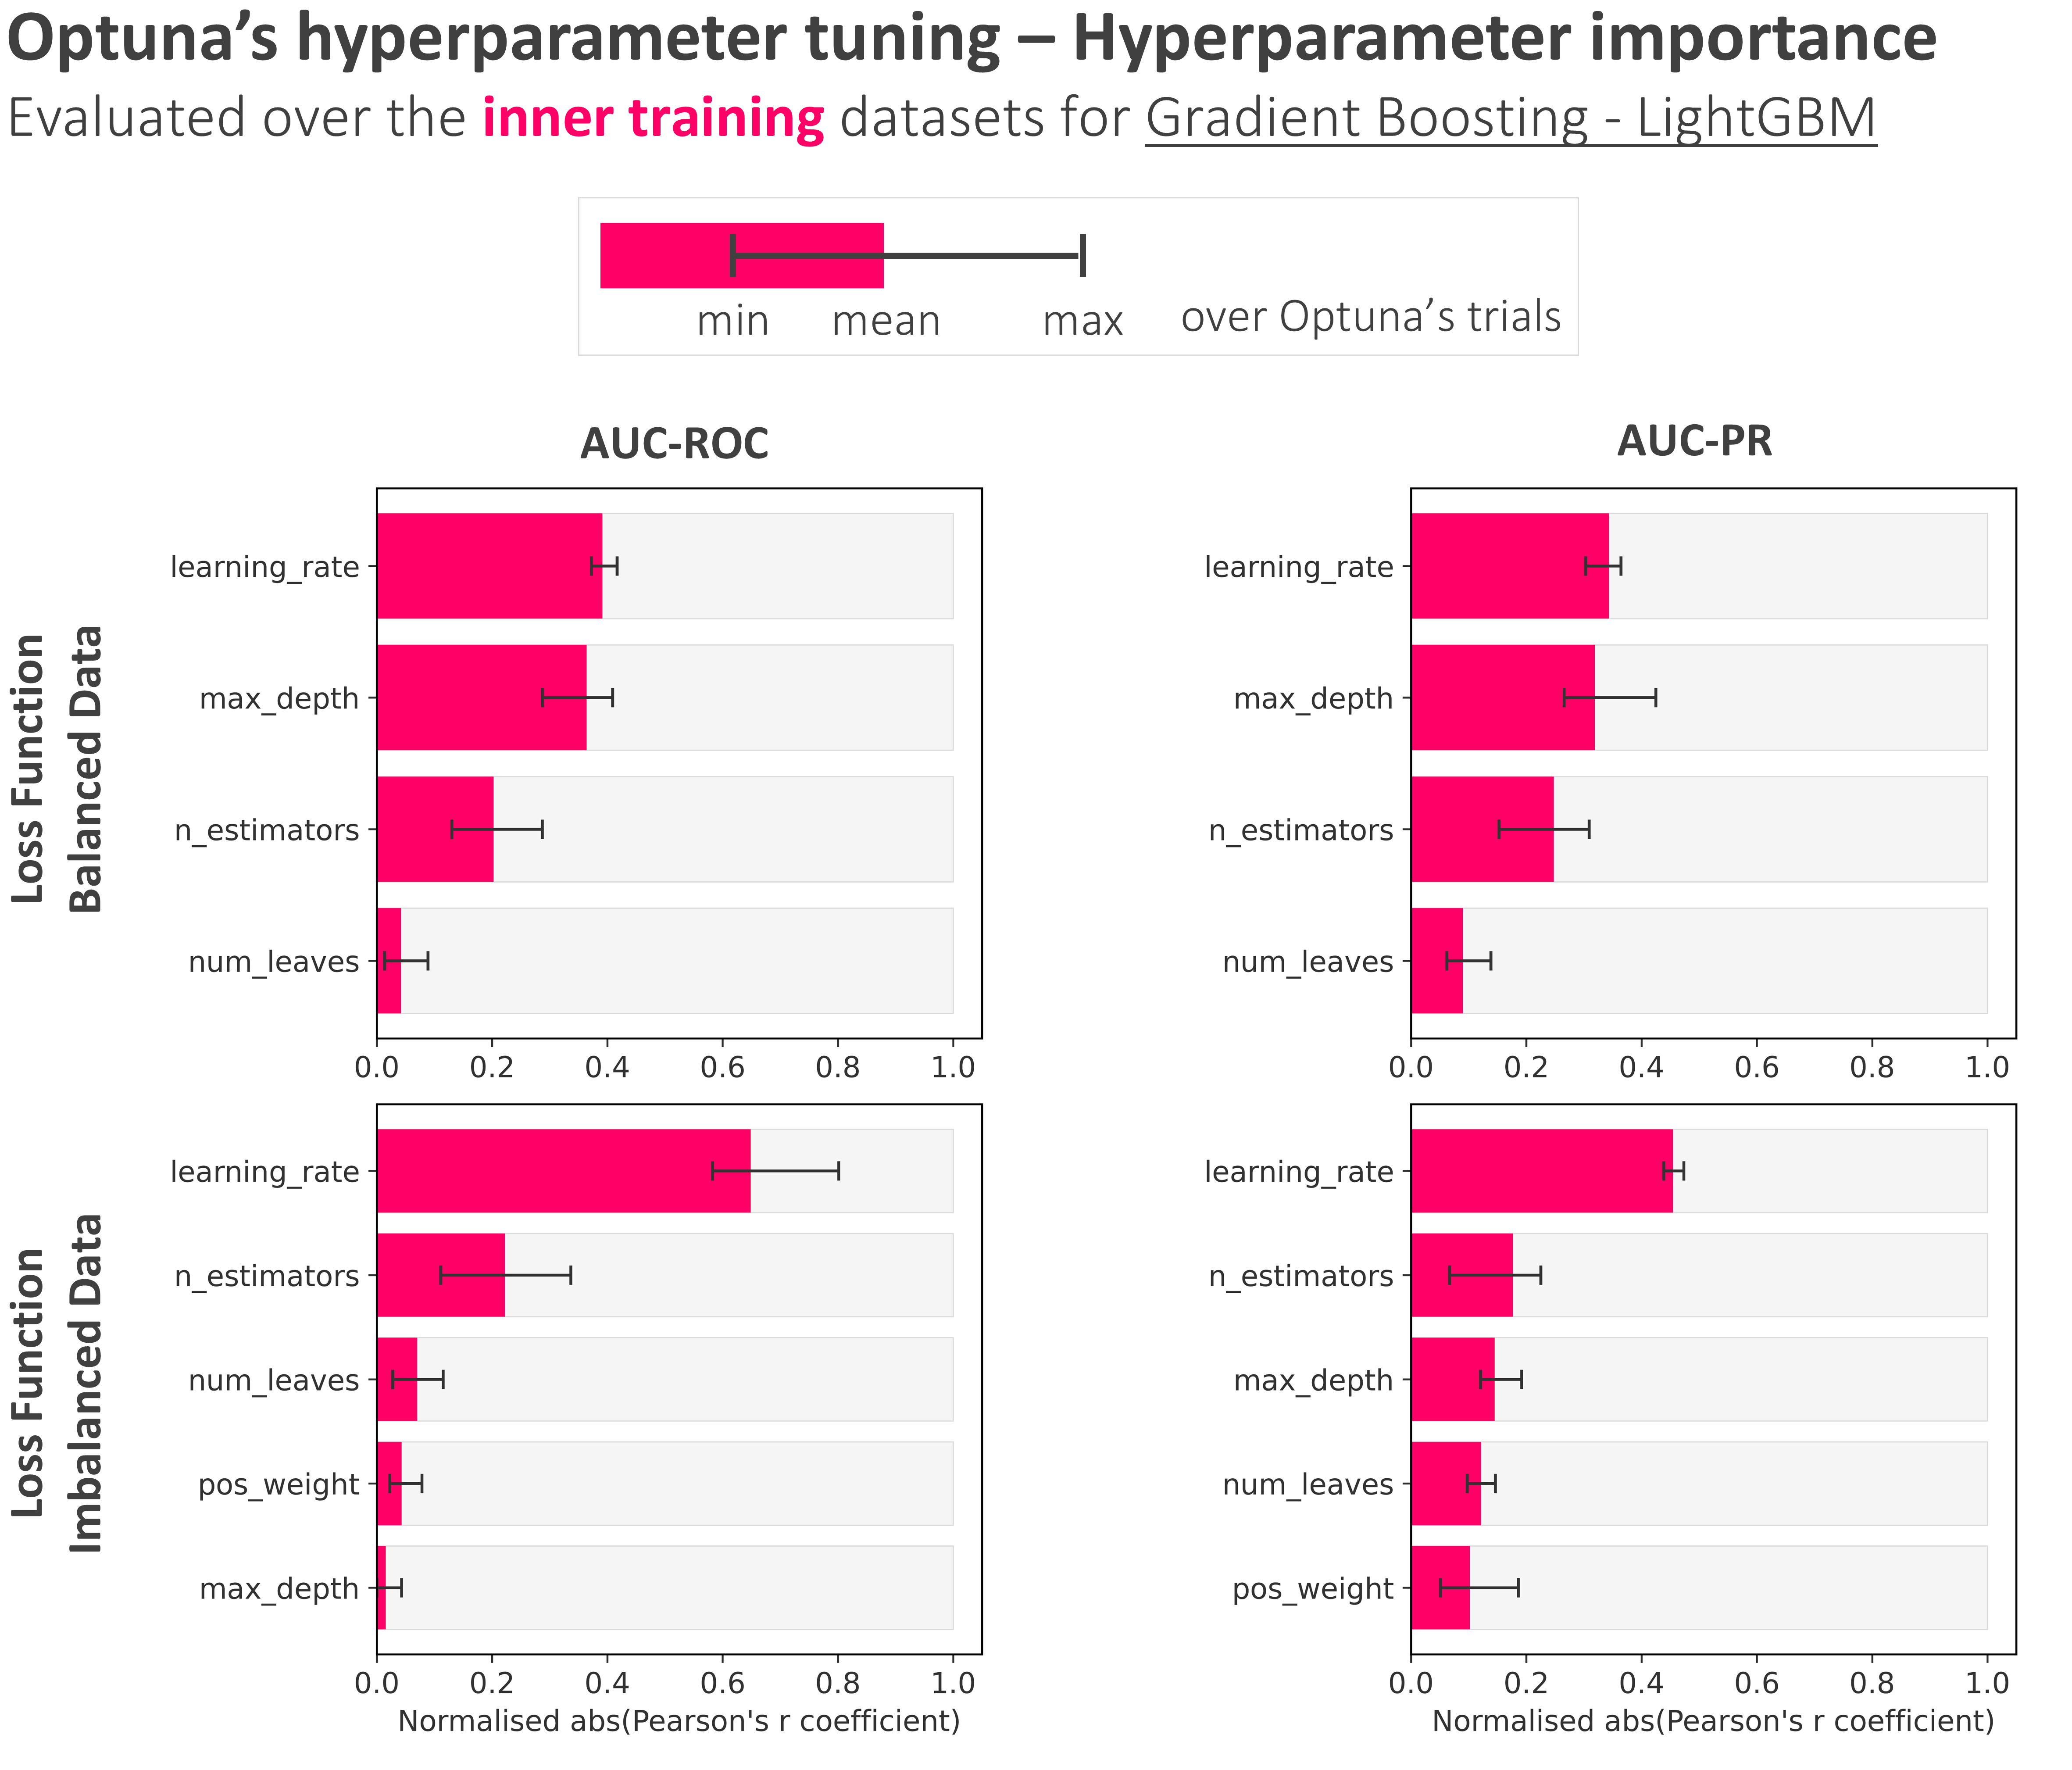
\includegraphics[width=12cm]{figures/optuna_parameters_importance_gradient_boosting_lightgbm.png}
\caption{\textbf{Optuna's hyperparameter importance for the LightGBM implementation of gradient boosting.} Similar to Figure \ref{fig:optuna_parameters_importance_gradient_boosting_xgboost}}
\label{fig:optuna_parameters_importance_gradient_boosting_lightgbm}
\end{figure*}

%f
\begin{figure*}[t]
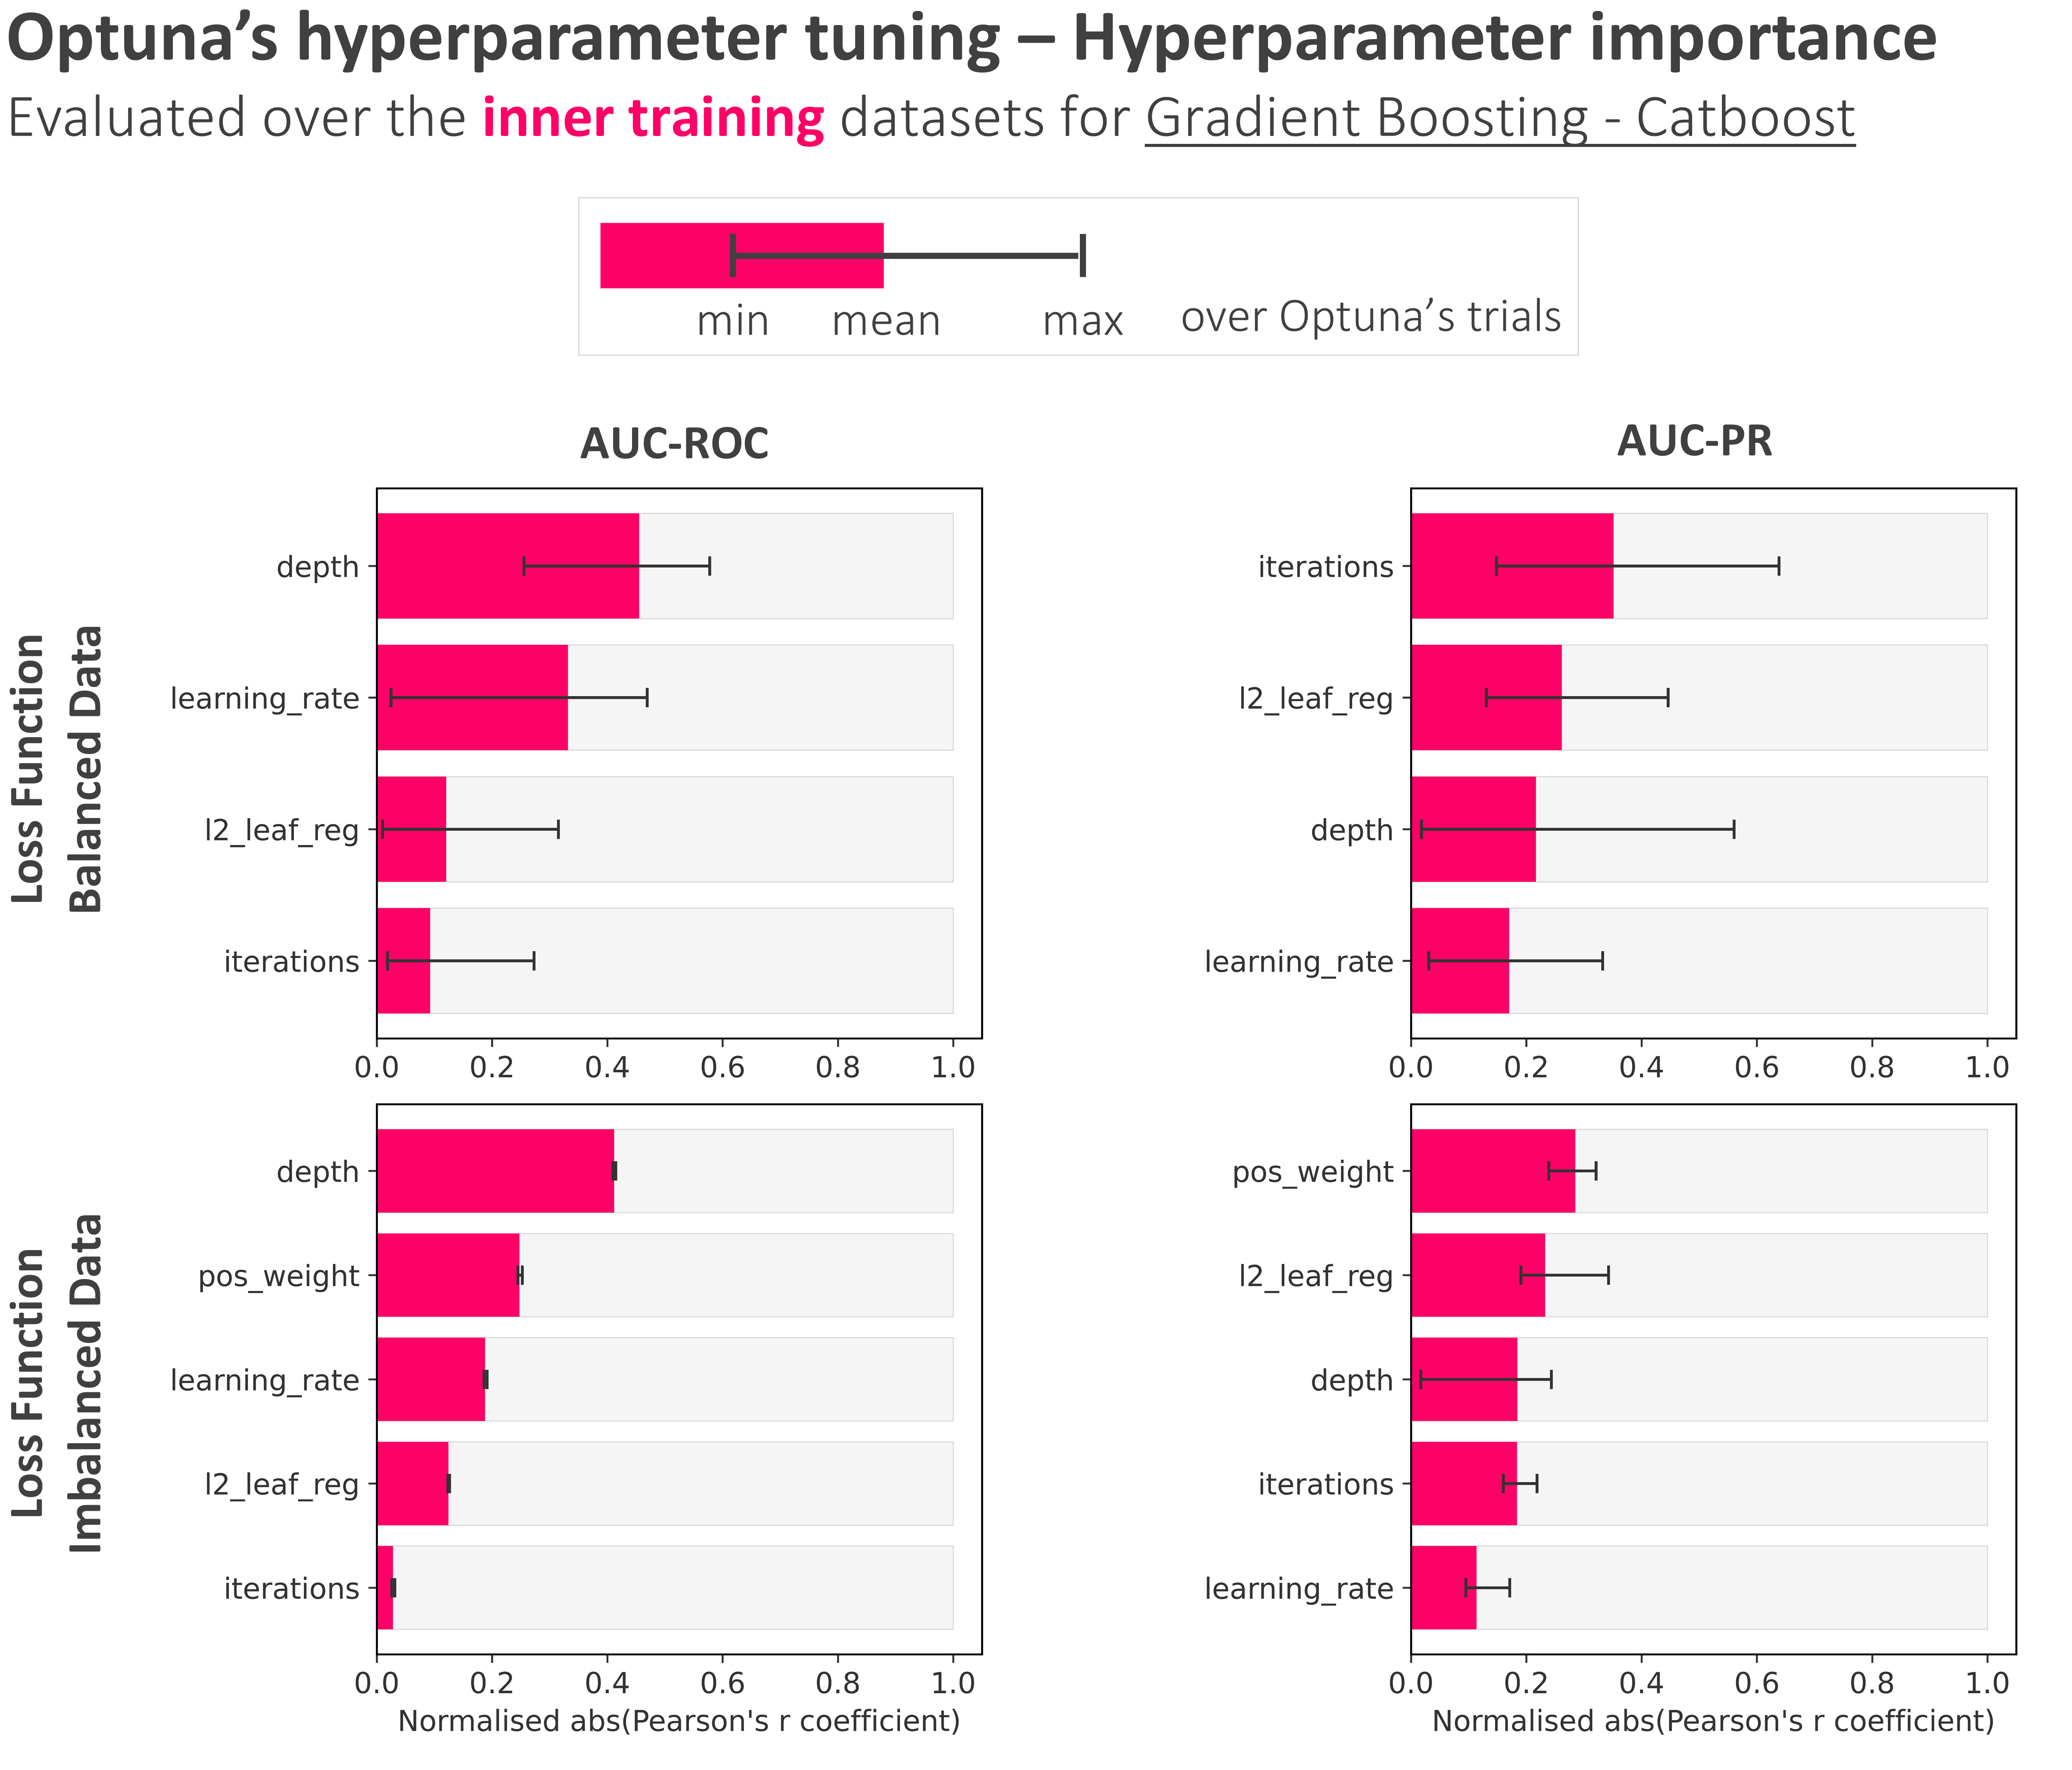
\includegraphics[width=12cm]{figures/optuna_parameters_importance_gradient_boosting_catboost.png}
\caption{\textbf{Optuna's hyperparameter importance for the CatBoost implementation of gradient boosting.} Similar to Figure \ref{fig:optuna_parameters_importance_gradient_boosting_xgboost}}
\label{fig:optuna_parameters_importance_gradient_boosting_catboost}
\end{figure*}

In contrast to gradient boosting implementations, random forest models exhibit inconsistent hyperparameter importance rankings across different loss functions and evaluation metrics, with parameters such as maximum depth, feature sampling ratios, and the number of estimators alternating in their relative influence depending on whether AUC-ROC or AUC-PR is optimised. This variability suggests that random forest hyperparameter spaces possess multiple viable configurations that achieve similar performance through different mechanisms (some configurations may excel through deeper individual trees, whilst others compensate with more aggressive feature sampling or a larger ensemble size), making the optimisation landscape more flexible but potentially more challenging to navigate systematically.

%f
\begin{figure*}[t]
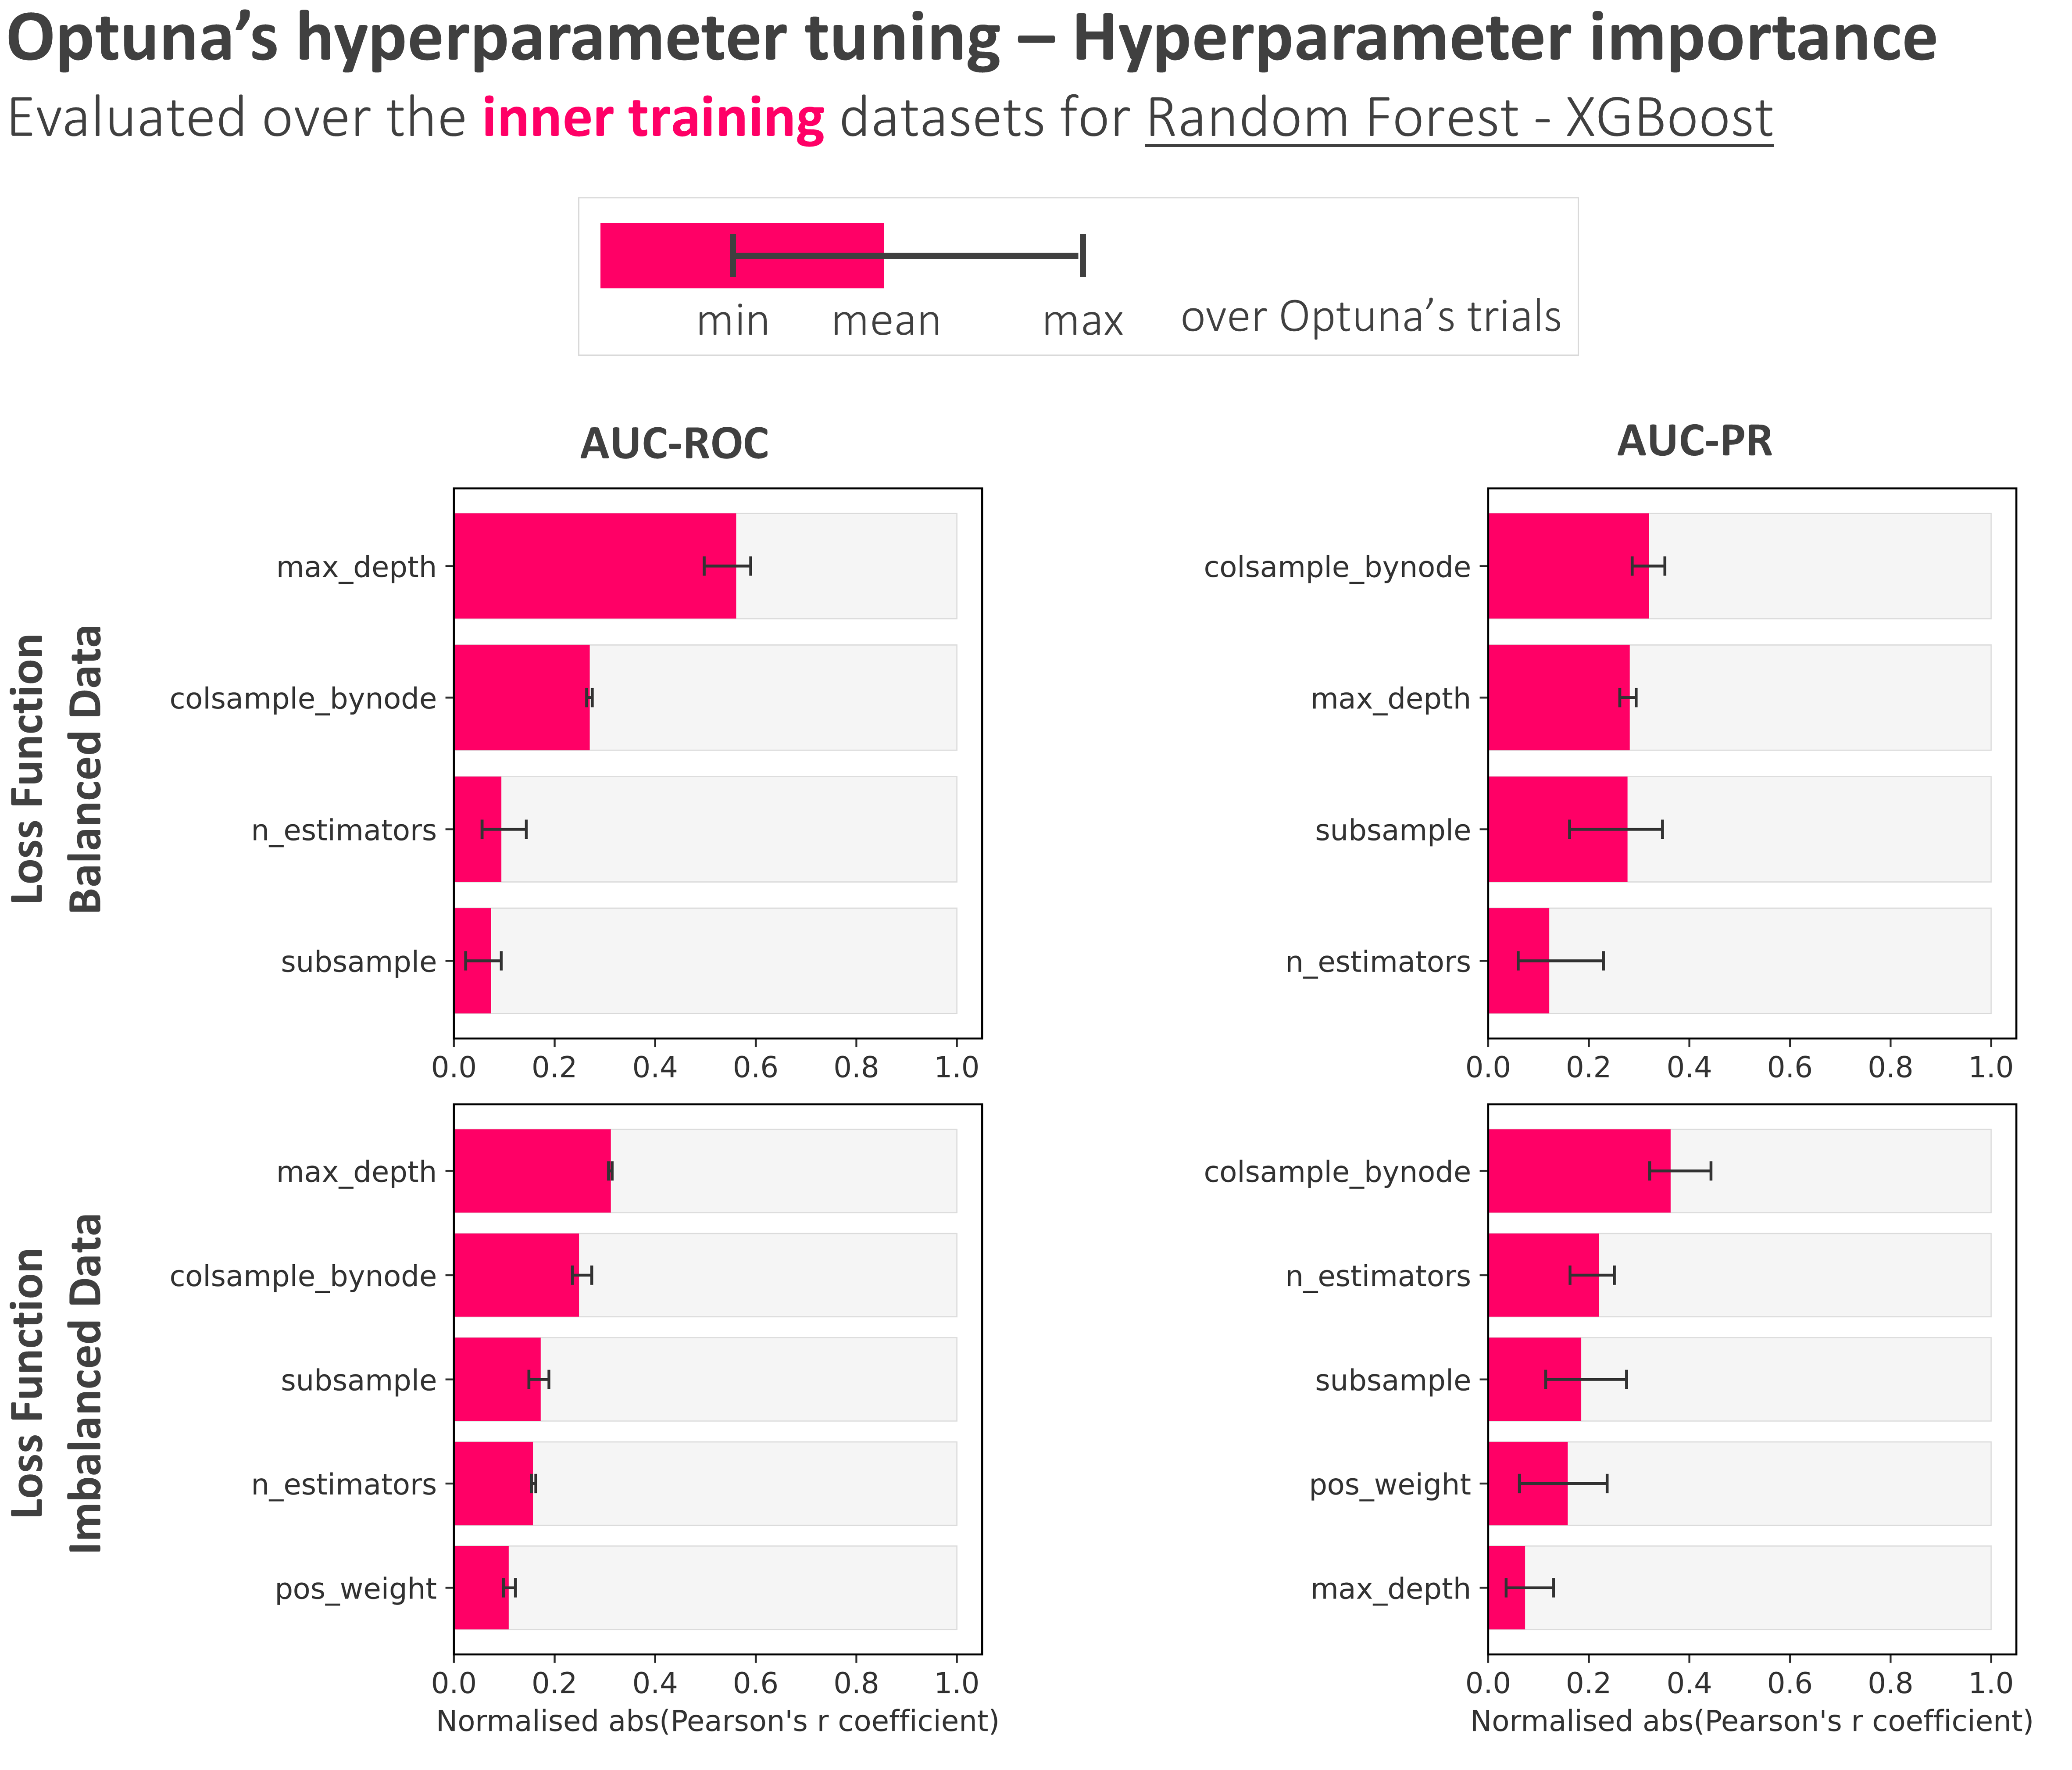
\includegraphics[width=12cm]{figures/optuna_parameters_importance_random_forest_xgboost.png}
\caption{\textbf{Optuna's hyperparameter importance for the XGBoost implementation of random forest.} Similar to Figure \ref{fig:optuna_parameters_importance_gradient_boosting_xgboost}}
\label{fig:optuna_parameters_importance_random_forest_xgboost}
\end{figure*}

%f
\begin{figure*}[t]
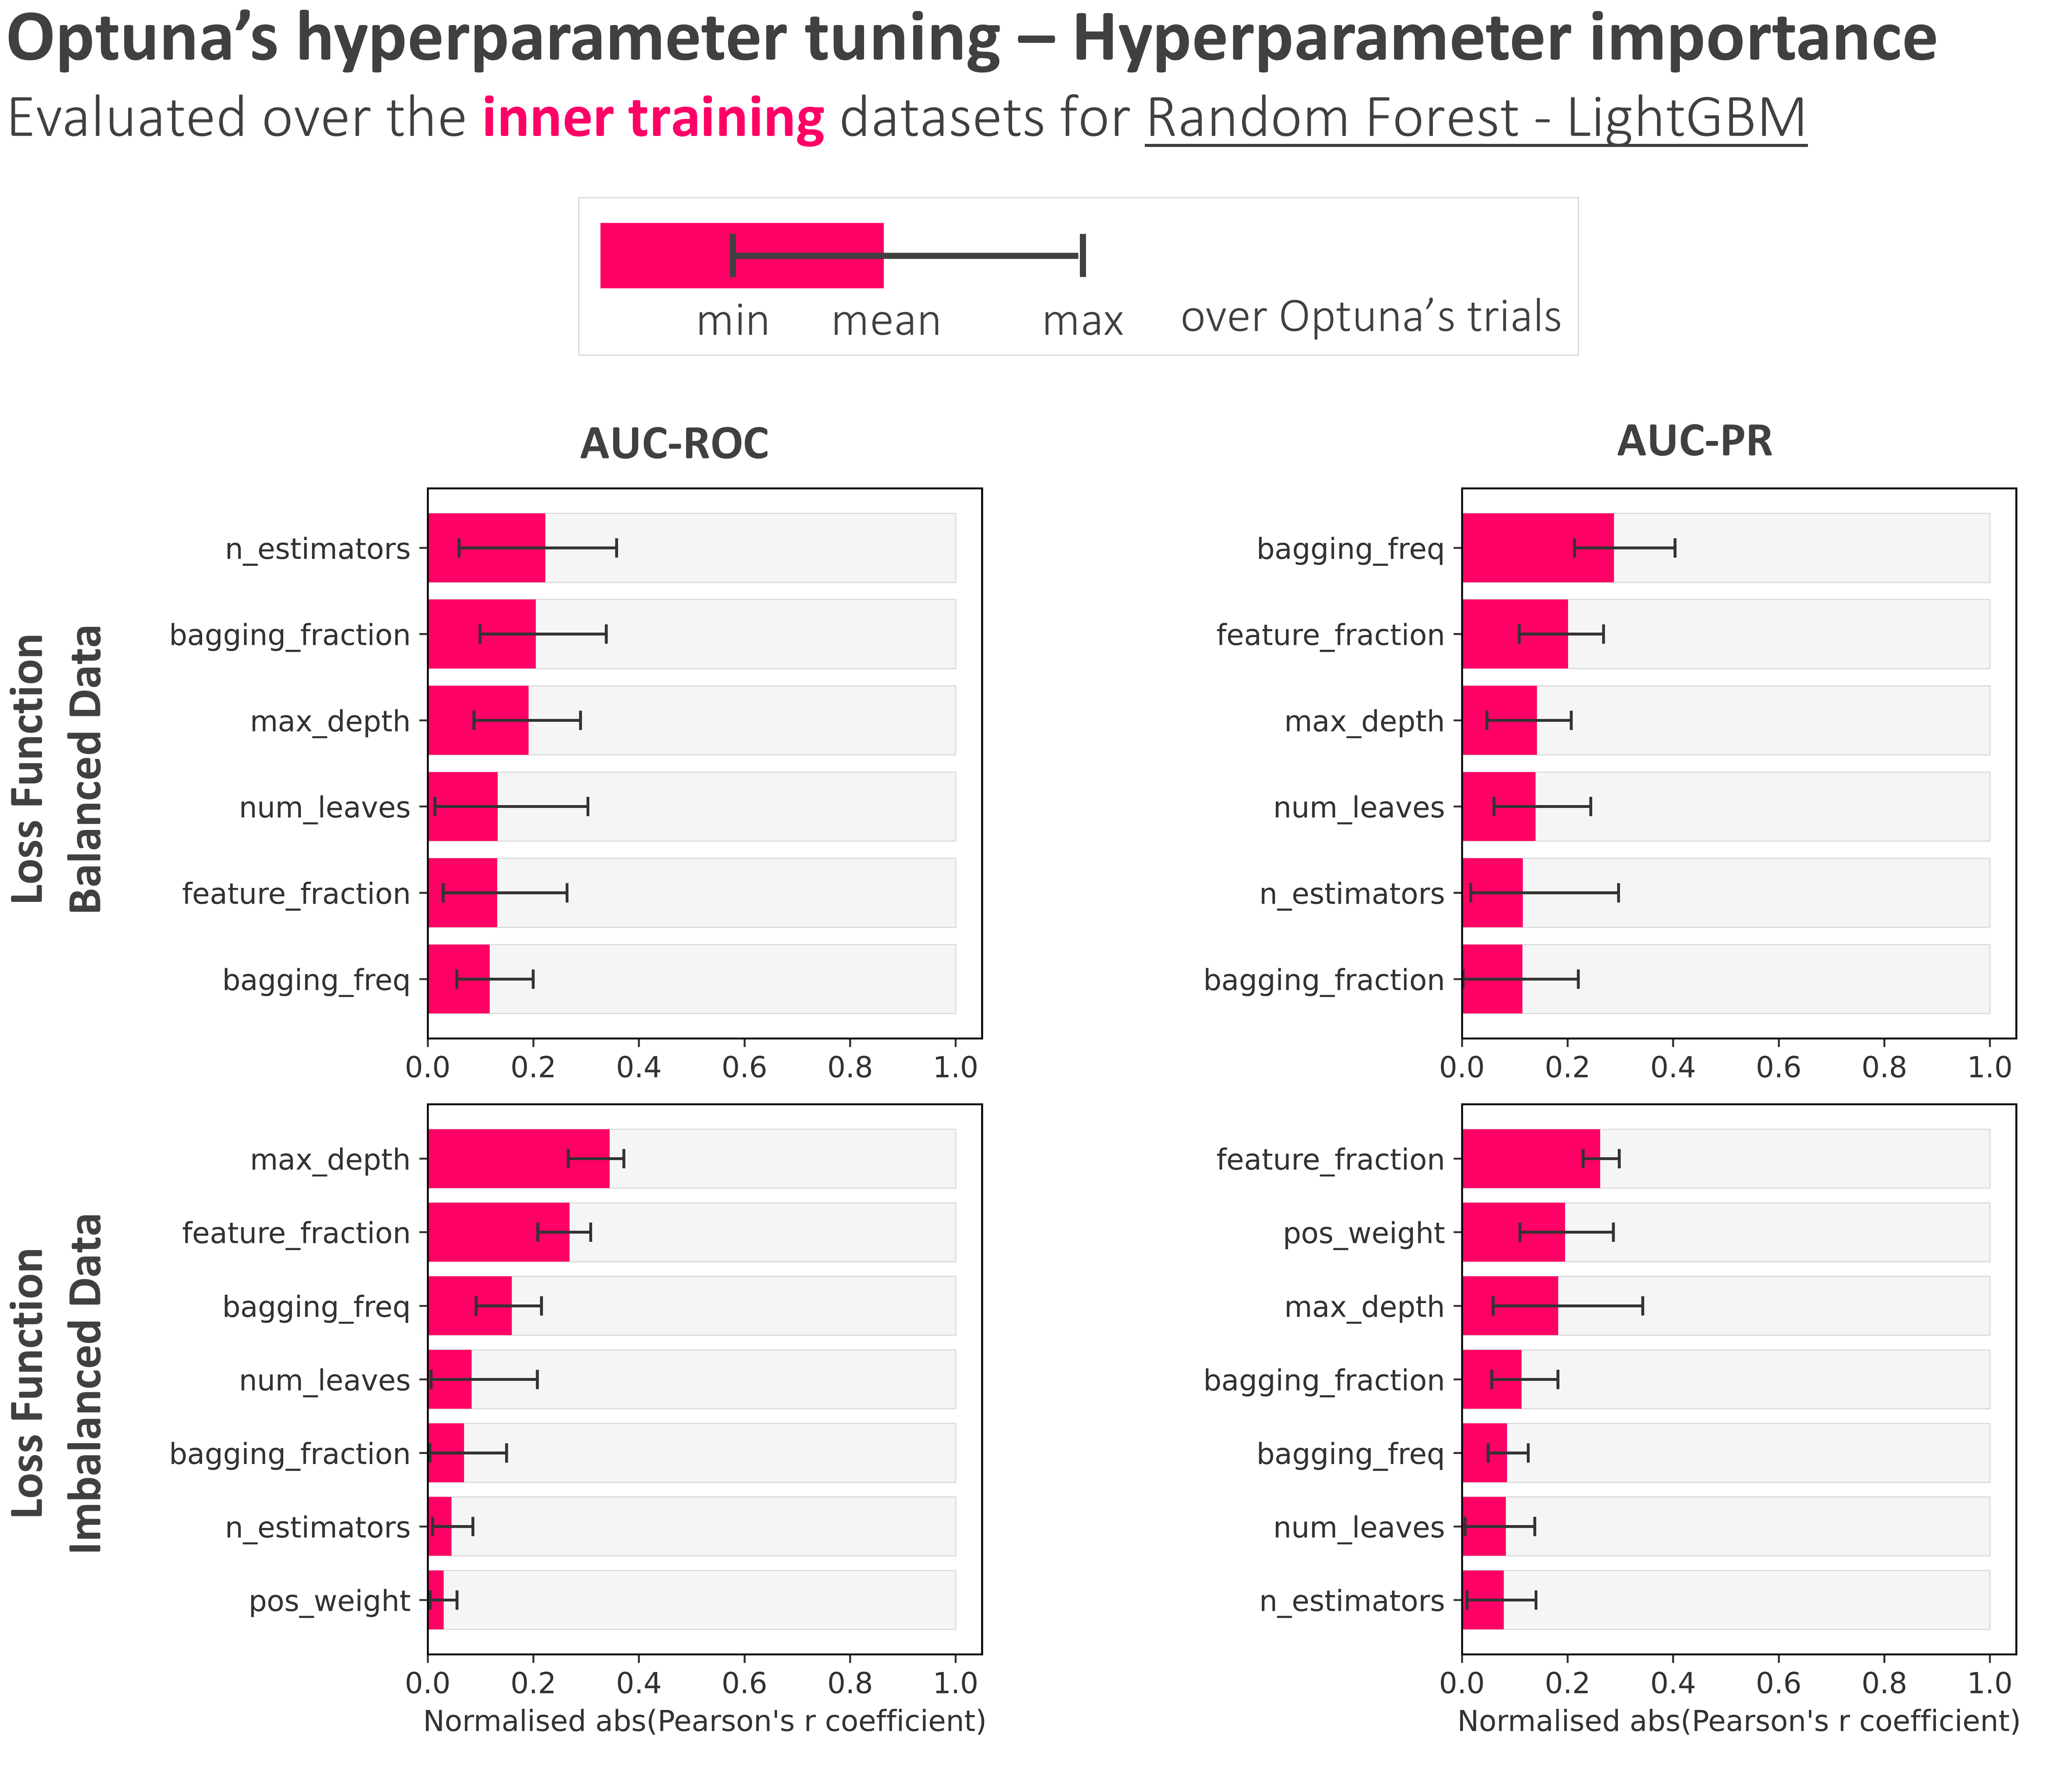
\includegraphics[width=12cm]{figures/optuna_parameters_importance_random_forest_lightgbm.png}
\caption{\textbf{Optuna's hyperparameter importance for the LightGBM implementation of random forest.} Similar to Figure \ref{fig:optuna_parameters_importance_gradient_boosting_xgboost}}
\label{fig:optuna_parameters_importance_random_forest_lightgbm}
\end{figure*}

The dominance of units\_0, dropout\_0, and learning rate for neural networks suggests that performance is primarily determined by the configuration of the first hidden layer, rather than the overall network depth. The parameter units\_0 controls the initial representational capacity, determining how effectively raw hydro-meteorological features are transformed into meaningful intermediate representations for detecting rare flash flood patterns. This layer must balance sufficient complexity to capture non-linear relationships whilst avoiding overfitting to the sparse positive examples. The high importance of dropout\_0 demonstrates that regularisation at this critical layer is essential for generalisation under extreme class imbalance. By randomly deactivating neurons during training, dropout forces the development of robust, redundant representations that prevent the model from memorising noise in the limited positive examples. The prominence of the learning rate parameter reflects the challenge of navigating an imbalanced dataset, where the gradient signal from rare positive examples can be easily overwhelmed by the abundance of negative cases. The diminished importance of deeper layer parameters suggests that shallow, well-regularised architectures may be the best choice for this application.

%f
\begin{figure*}[t]
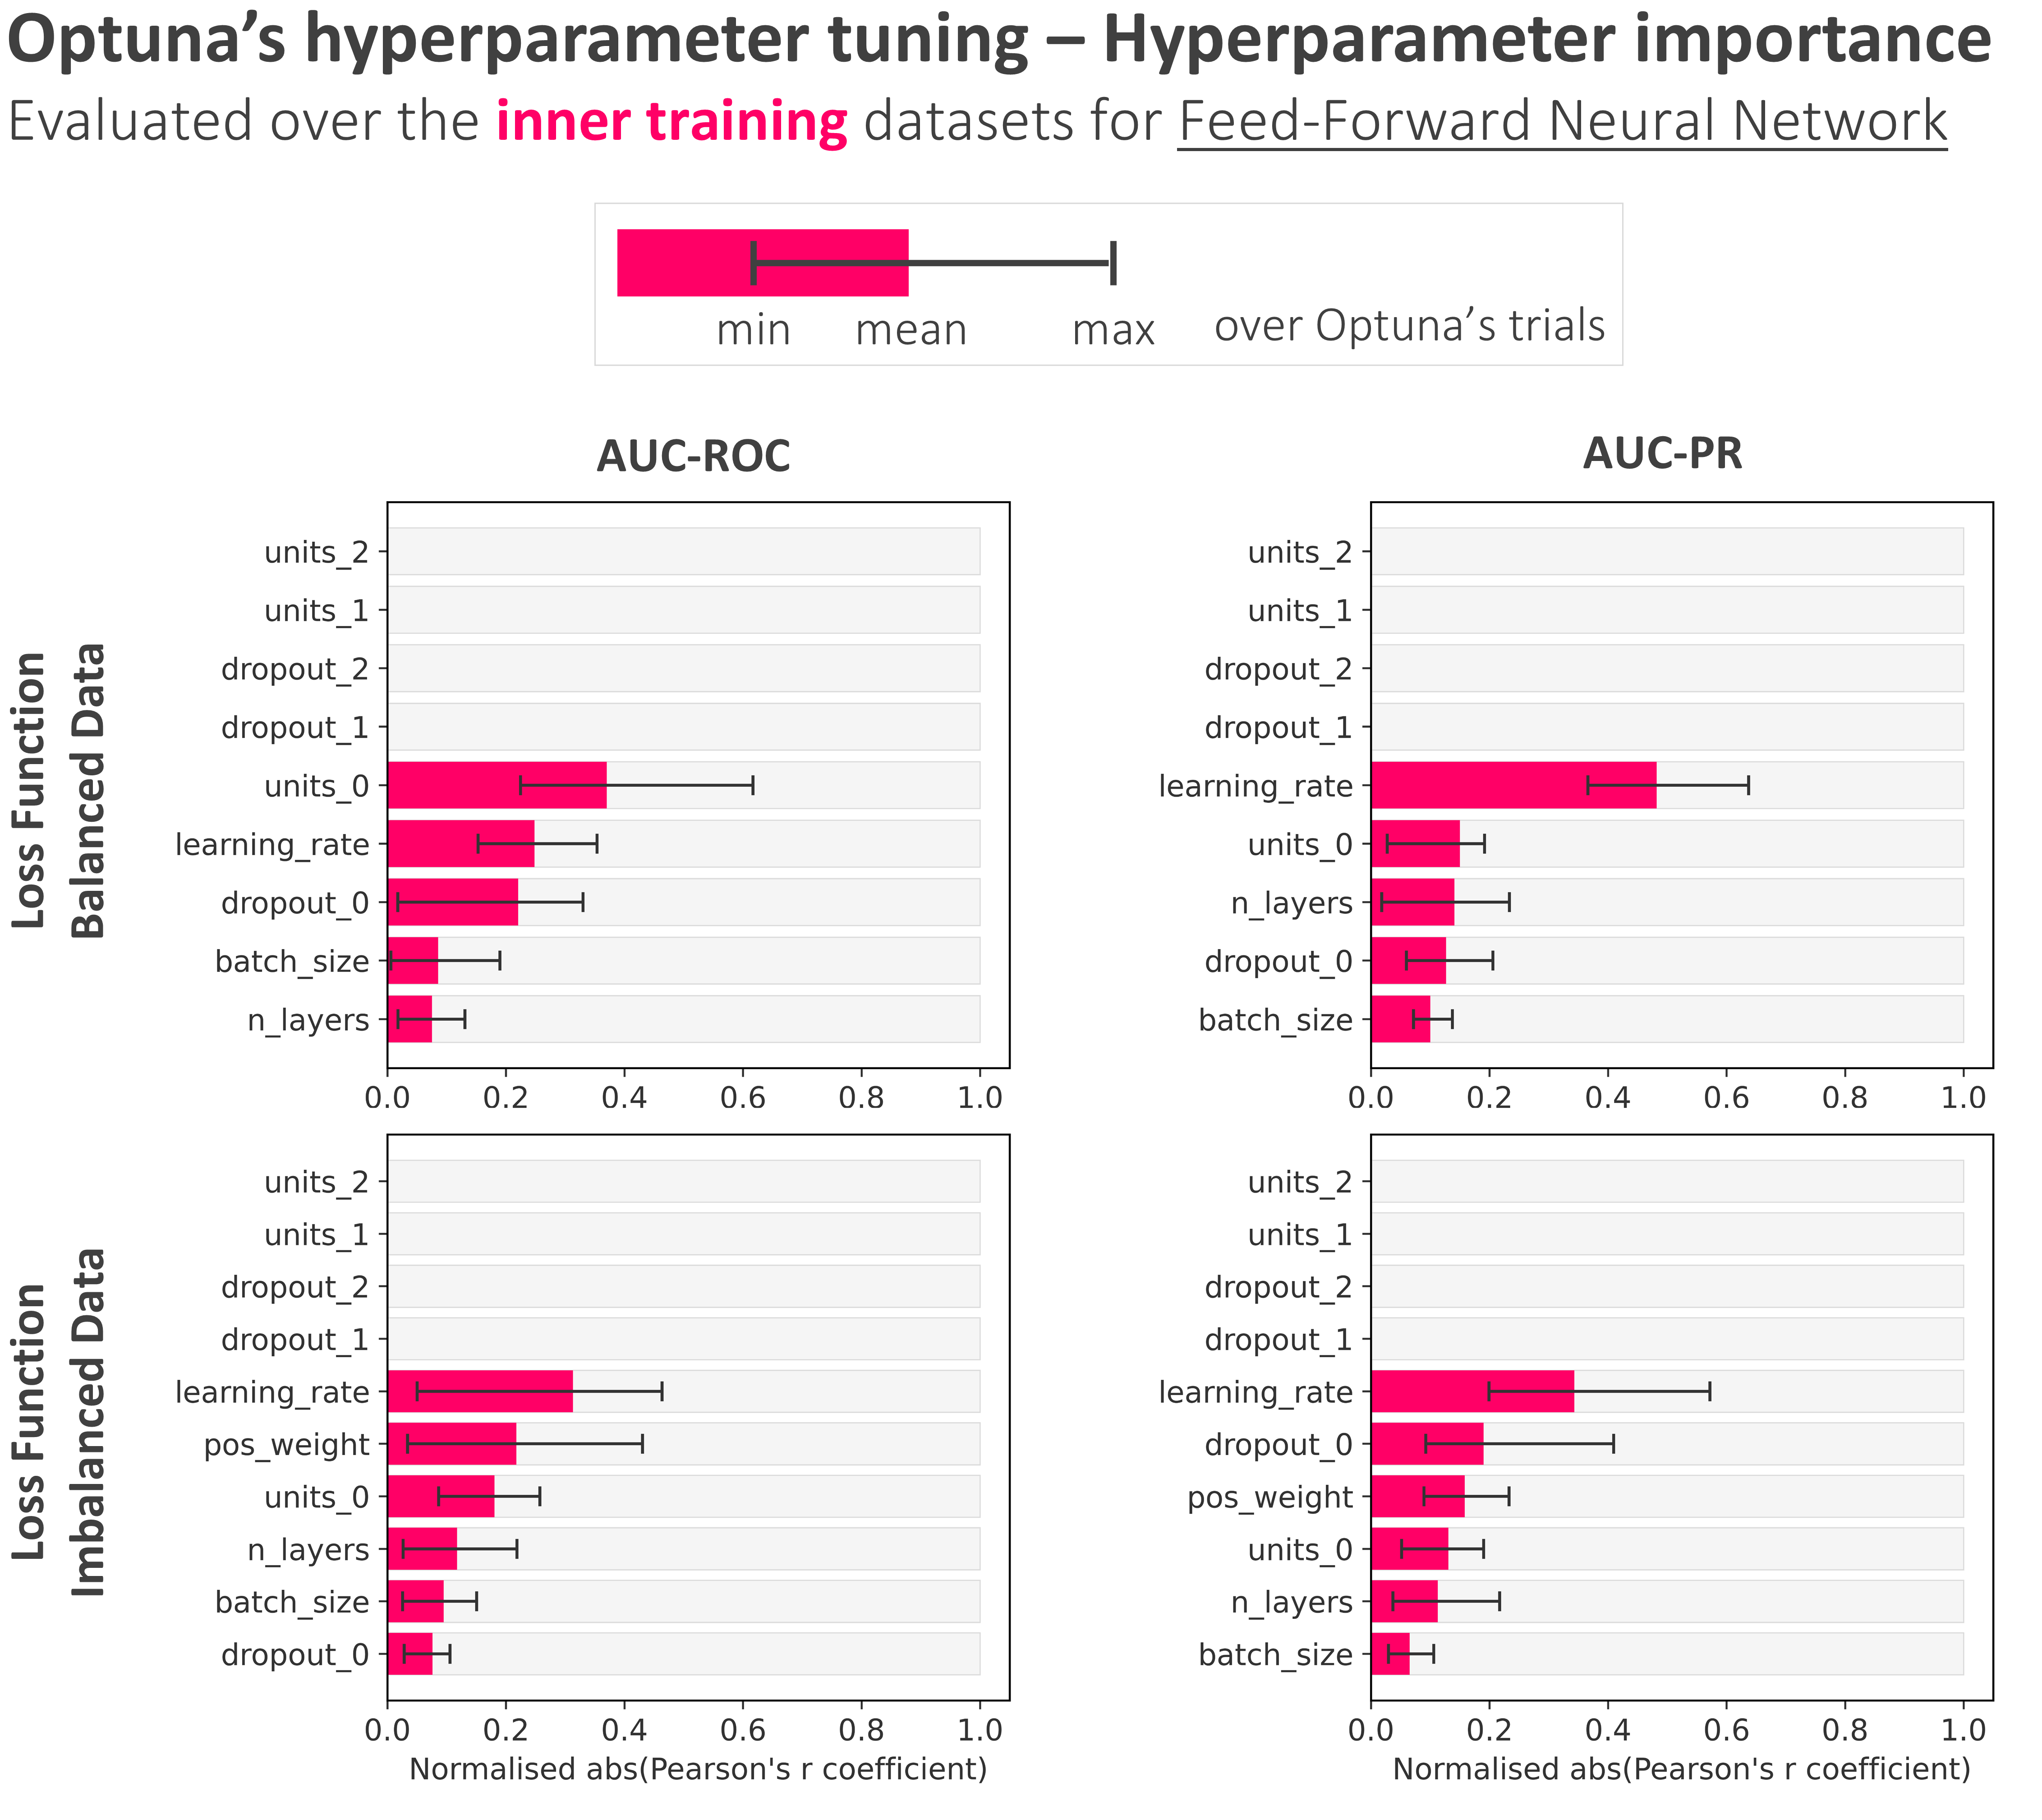
\includegraphics[width=12cm]{figures/optuna_parameters_importance_feed_forward_nn.png}
\caption{Optuna's hyperparameter importance for feed-forward neural network. Similar to Figure \ref{fig:optuna_parameters_importance_gradient_boosting_xgboost}}
\label{fig:optuna_parameters_importance_feed_forward_nn}
\end{figure*}


\subsection{Verification results over reanalysis data}

To assess the generalisation capabilities of the trained data-driven models, this section compares various performance metrics (presented in Section ? between the training dataset, with data from 2001 to 2020, and the independent verification dataset, with data from 2021 to 2024.

All data-driven models exhibit relatively stable AUC-ROC values around 0.8 for the verification dataset with minimal decrease from the AUC-ROC values obtained for the training dataset (Figure \ref{fig:verif_training_test_overall}, first column). This behaviour is constant across both evaluation metrics (AUC-ROC and AUC-PR) and both types of loss function (general for balanced datasets and specific for imbalanced datasets). Hence, all data-driven models show an overall discrimination ability that generalises well from training to verification datasets. The AUC-PR values demonstrate more variability across data-driven models (Figure \ref{fig:verif_training_test_overall}, second column), with CatBoost showing the highest estimates overall, especially when hyperparameters are tuned maximising the AUC-ROC evaluation metric (for both types of loss function). For all models, however, values of AUC-PR remain relatively small (Close to 0). Even though all models show a tendency to slightly overestimate the frequency of areas at risk of flash flood (FB just above 1, Figure \ref{fig:verif_training_test_overall}, third column), the FB values also show high variability across the data-driven models. When considering the generic loss function, the XGBoost and LightGBM implementations for random forest and gradient boosting obtain the closest values to 1, but increase of ~20\% when considering the loss function specific for imbalanced datasets, showing even greater FB than the other tested models (which maintain similar values than those obtained when considering the generic loss function).

%f
\begin{figure*}[t]
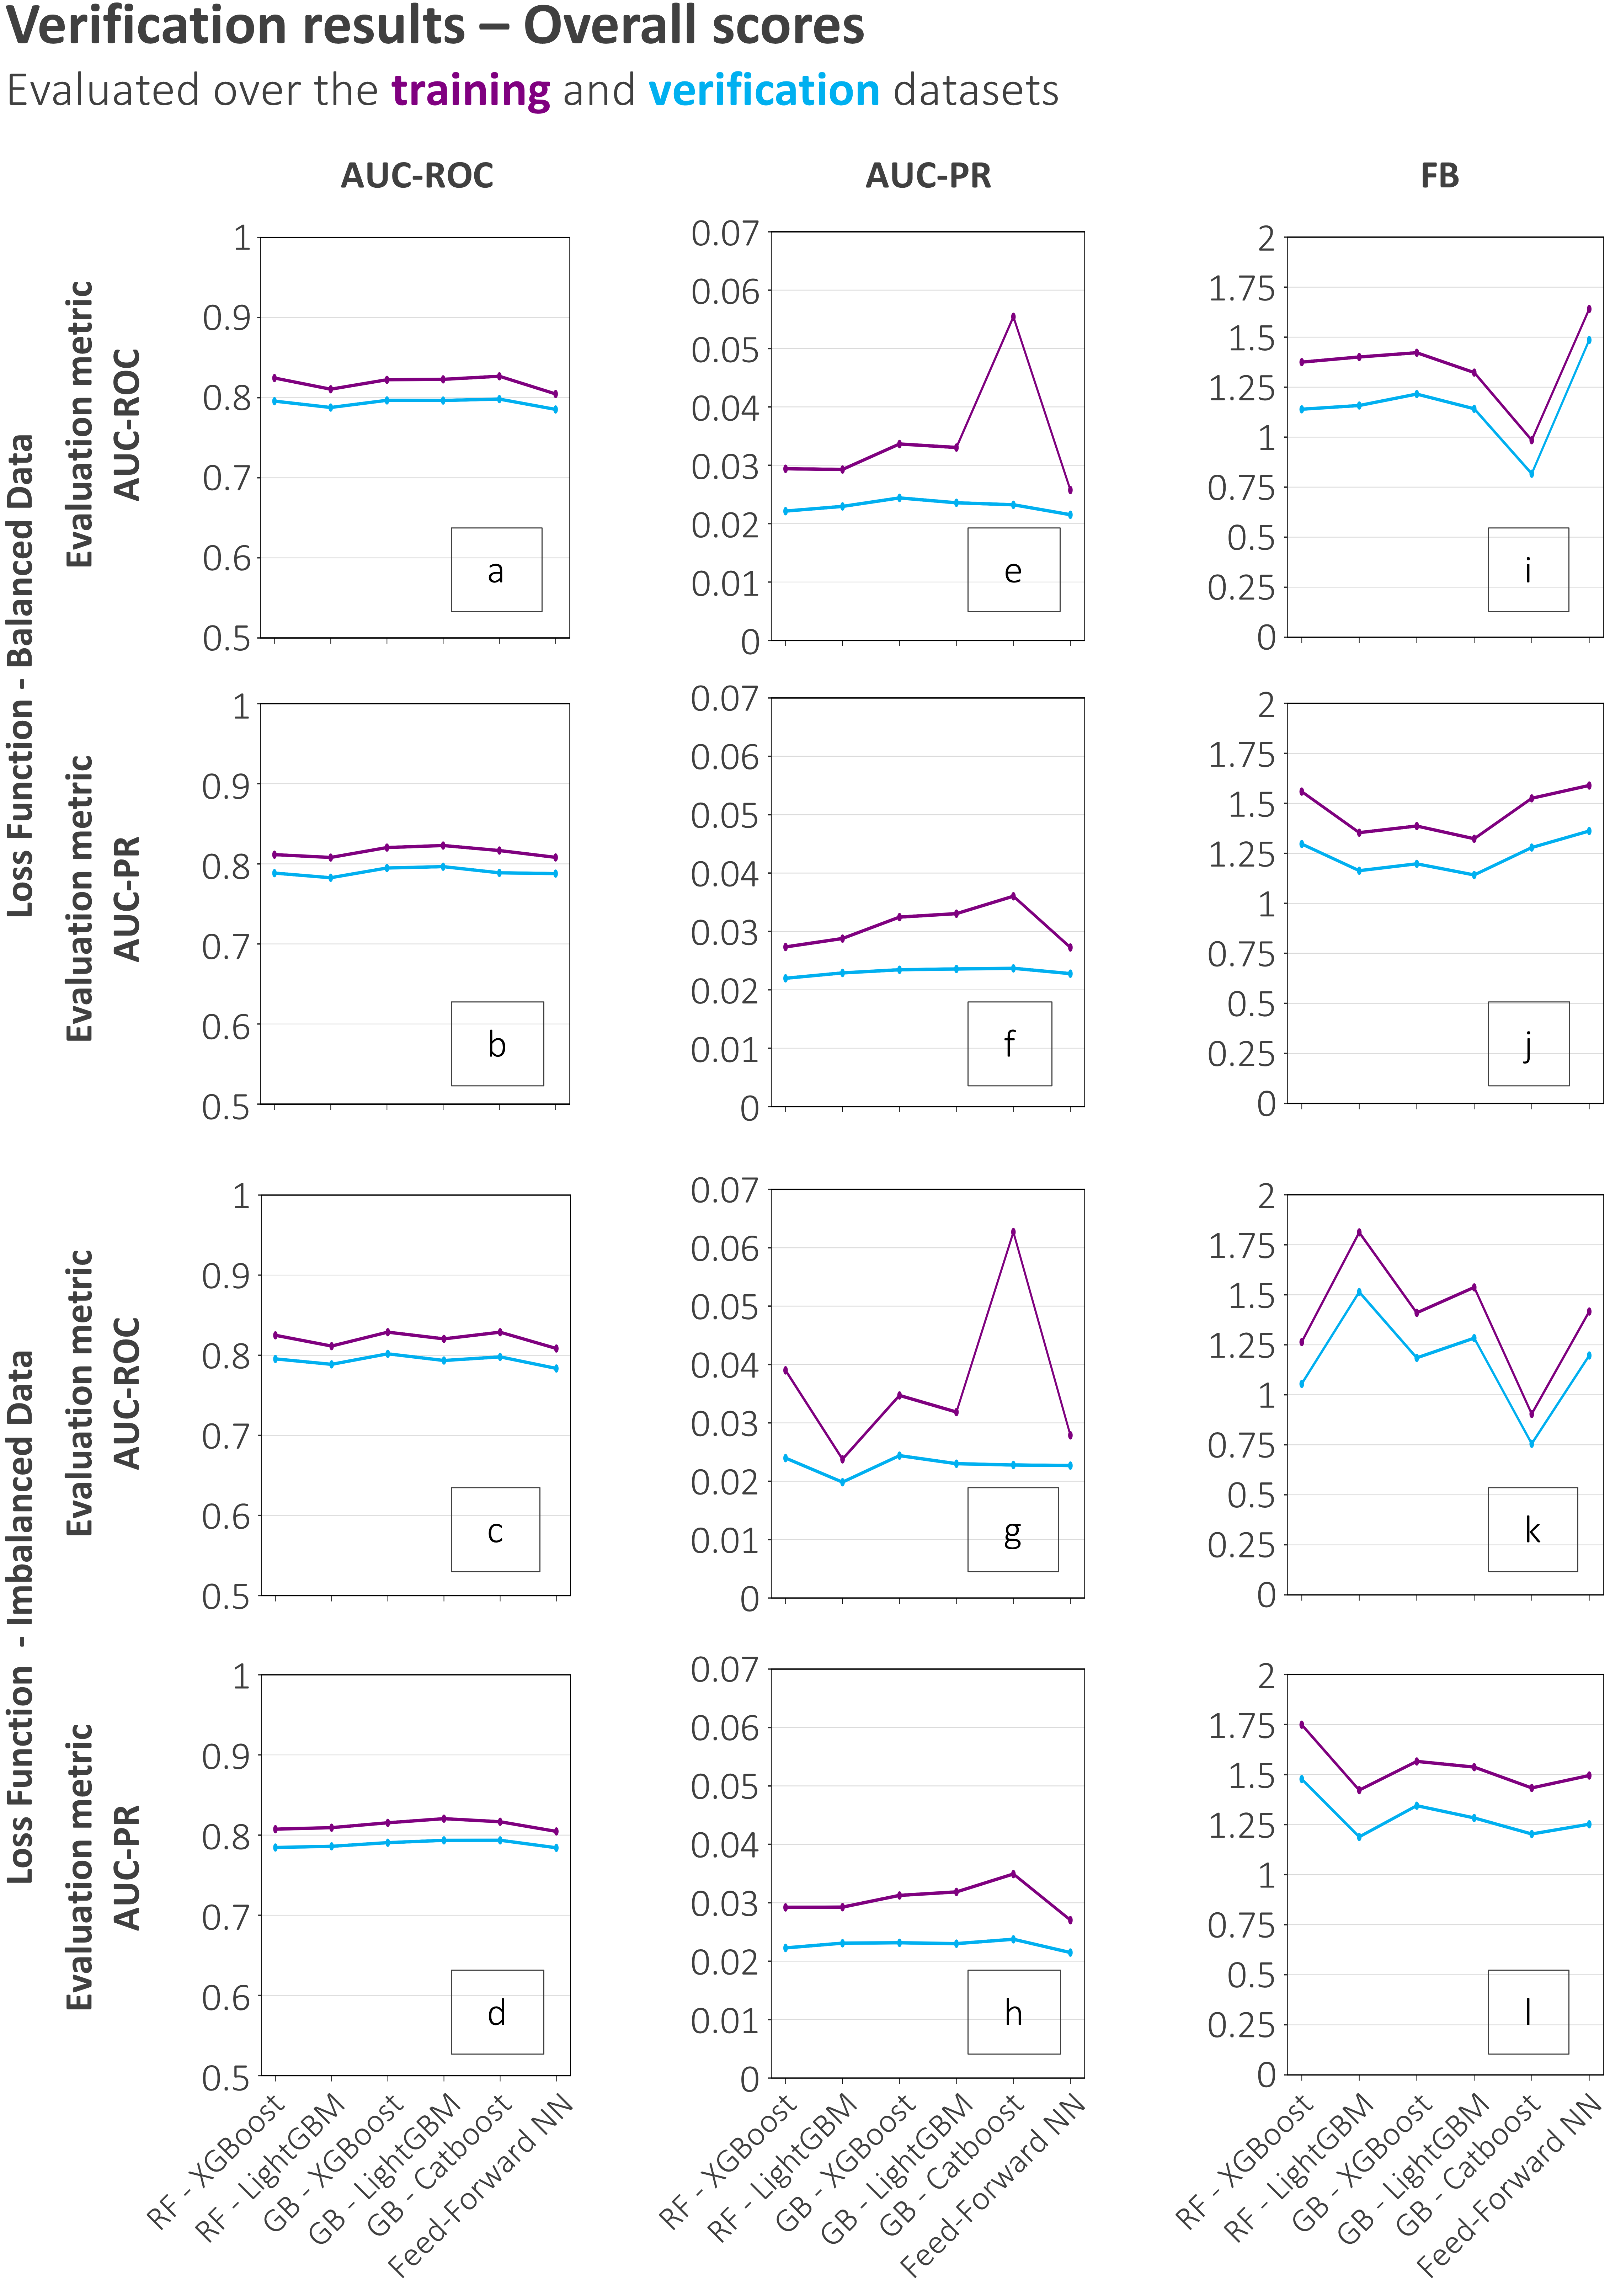
\includegraphics[width=12cm]{figures/verif_training_test_overall.png}
\caption{\textbf{Verification results: overall scores} The first, second, and third columns show, respectively, the estimates for the area under the ROC curve (AUC-ROC), the area under the precision-recall curve (AUC-PR), and the frequency bias (FB) for the six considered data-driven models. The estimates of the overall verification scores are shown for the \textcolor{colourTraining}{training dataset} and the \textcolor{colourTest}{verification dataset}. Results are presented for the models trained considering both types of loss functions and evaluation metrics.}
\label{fig:verif_training_test_overall}
\end{figure*}

Overall, ROC curves exhibit minimal degradation between training datasets and verification datasets (Figure \ref{fig:verif_training_test_breakdown_roc_curve}). The ROC curve, however, reveals distinct patterns between models trained with balanced \ref{fig:verif_training_test_breakdown_roc_curve}a-f and m-r) versus imbalanced loss functions \ref{fig:verif_training_test_breakdown_roc_curve}g-l and s-x). The ROC curves computed for models employing balanced loss functions maintain a remarkably consistent shape across all data-driven models and evaluation metrics, as well as a consistent relative difference between ROC curves computed using the 1\% discretisation (solid lines) and the 0.01\% (dashed lines). The former ROC curves yield lower AUC-ROC values than the latter due to the "truncation effect" caused by stopping the ROC curve at the 1\% probability threshold. The same does not hold when considering models trained with weighted loss functions, except for CatBoost. These ROC curves achieve higher hit rates, e.g., ~0.9 for the XGBoost and LightGBM implementations of gradient boosting (Figures \ref{fig:verif_training_test_breakdown_roc_curve}i-j) and ~0.6 for the feed-forward neural network (Figures \ref{fig:verif_training_test_breakdown_roc_curve}l) compared to 0.4 for their balanced counterparts (Figures \ref{fig:verif_training_test_breakdown_roc_curve}c-d and f), but at the cost of much higher false alarm rates, e.g., ~0.5 for XGBoost and LightGBM an ~0.2 for the feed-forward neural network compared to 0.025 in their balanced counterparts. Whilst XGBoost and LightGBM implementations of gradient boosting and the feed-forward neural network show consistent patterns across evaluation metrics, the random forest implementations display metric-dependent responses. Specifically, LightGBM Random Forest shows the altered behaviour when optimised for AUC-ROC, whereas XGBoost Random Forest responds differently under AUC-PR.

%f
\begin{figure*}[t]
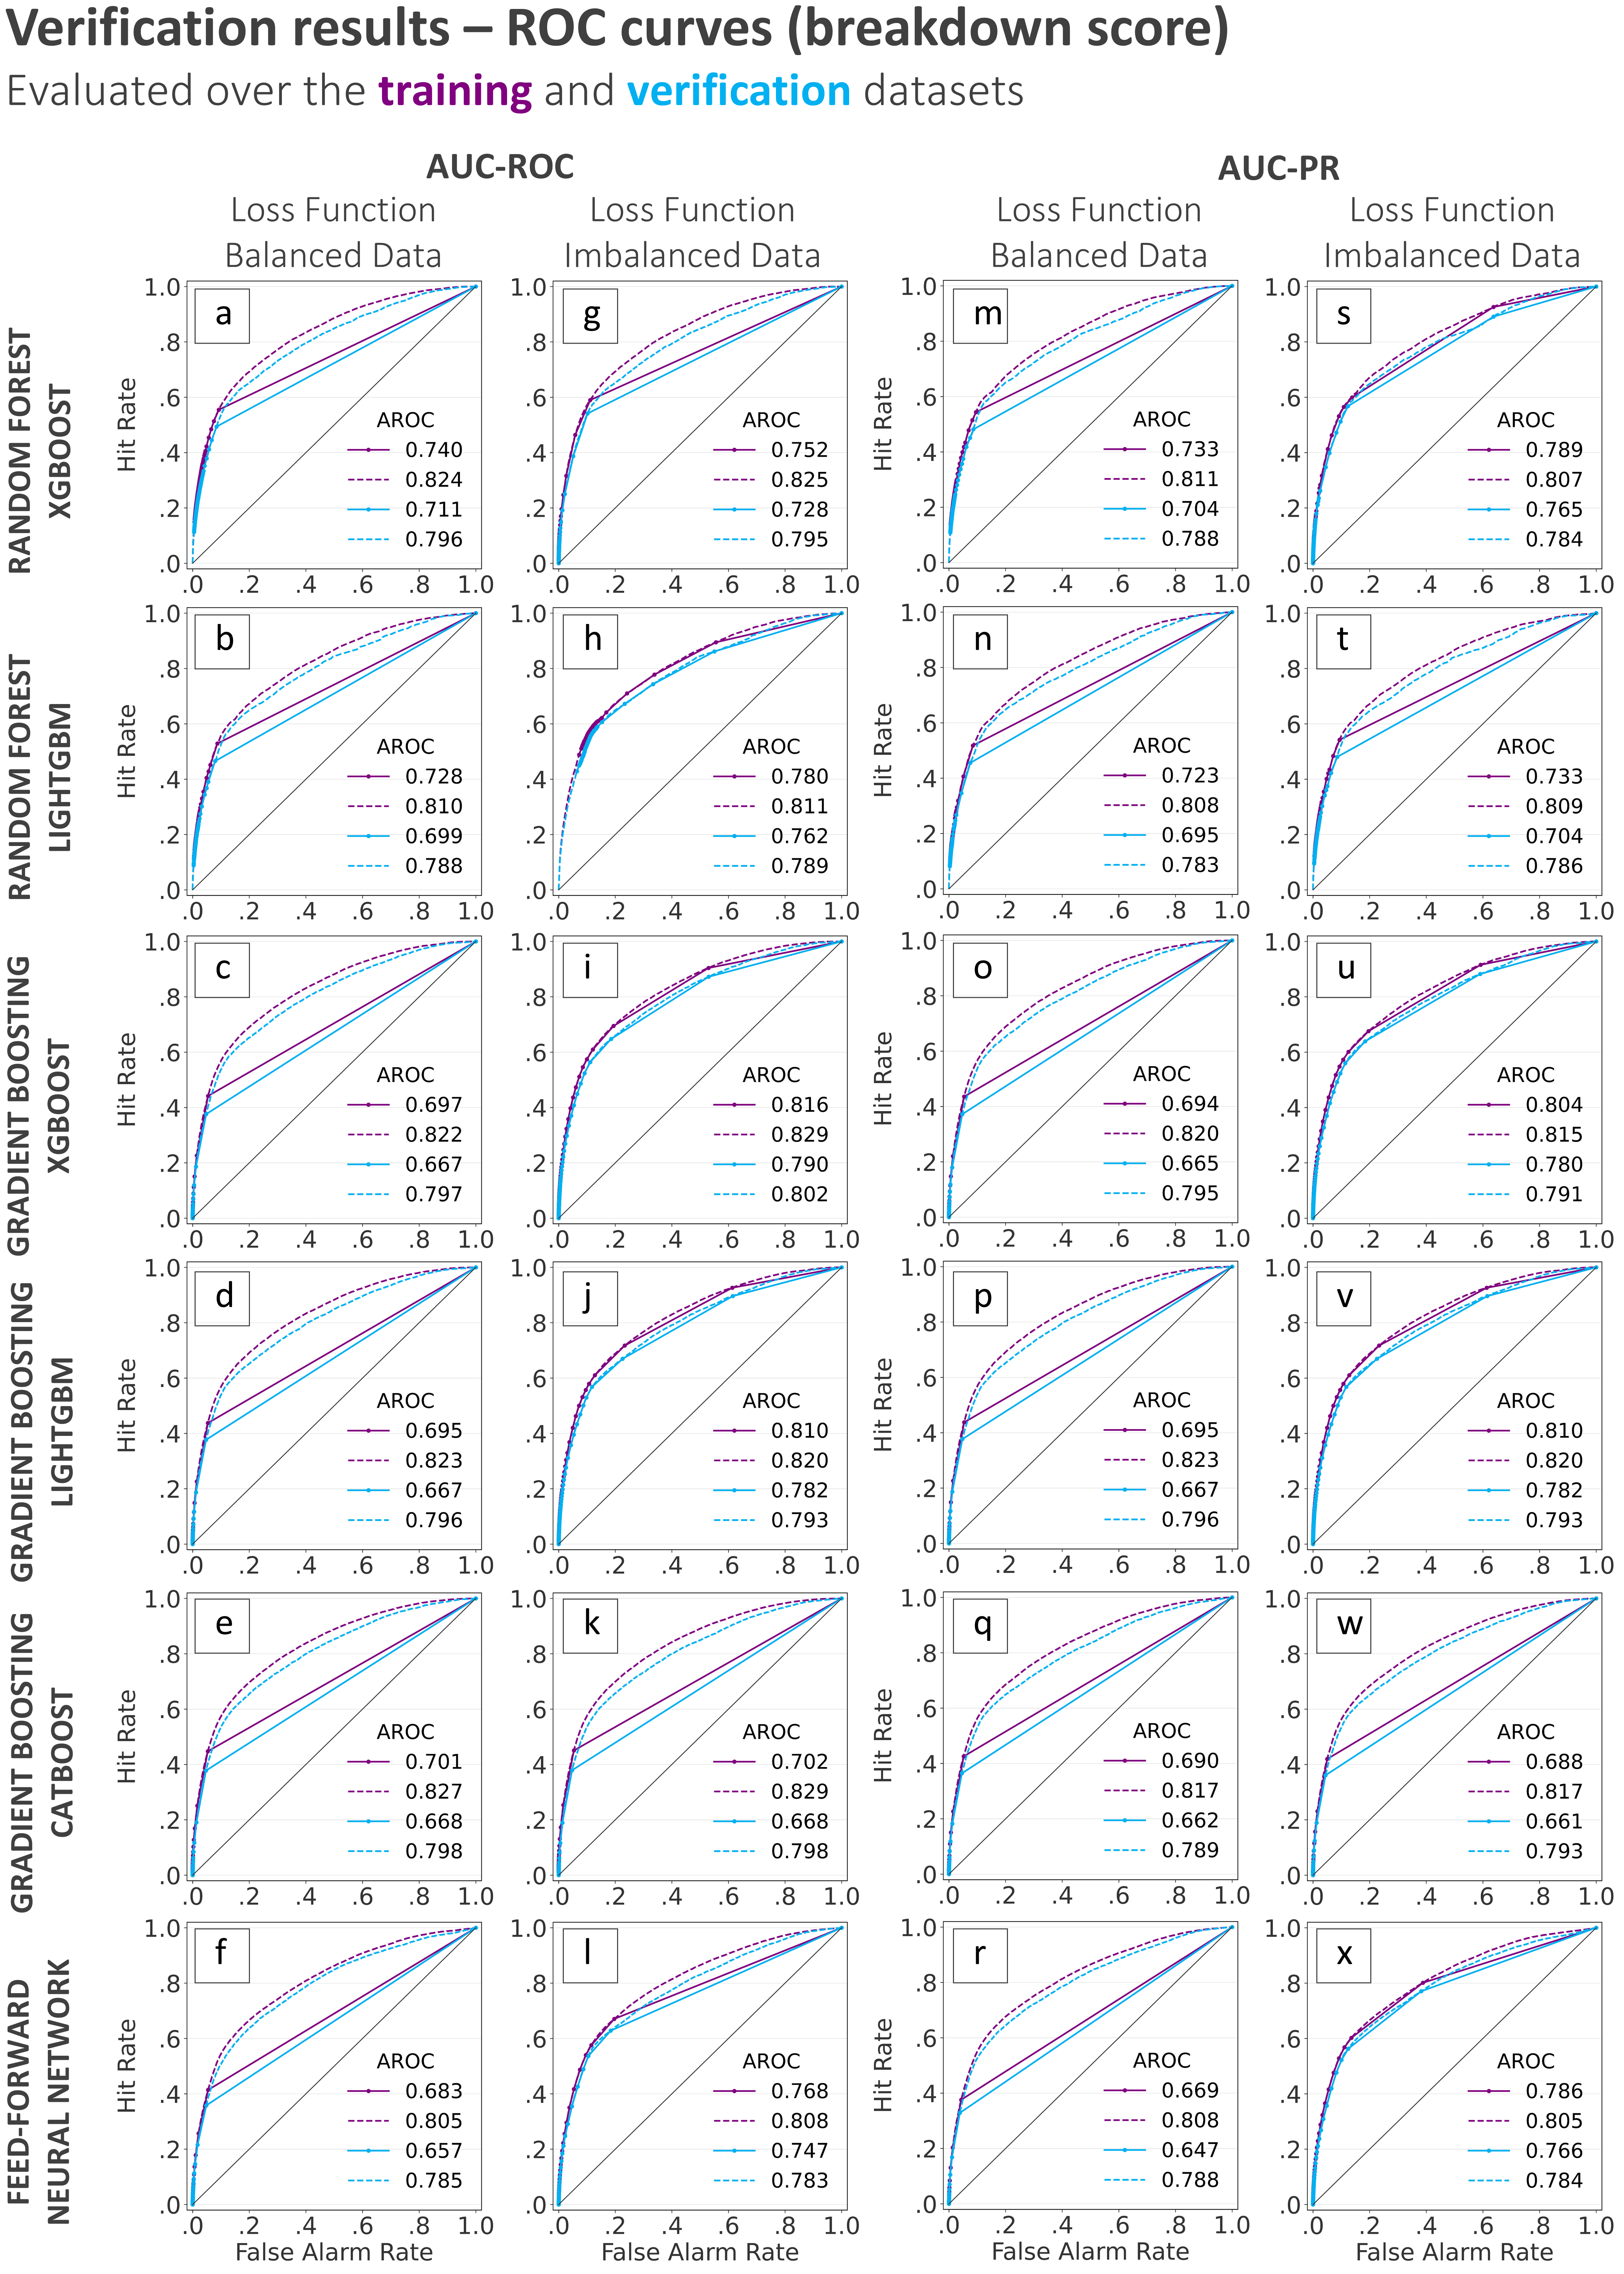
\includegraphics[width=12cm]{figures/verif_training_test_breakdown_roc_curve.png}
\caption{\textbf{Verification results: breakdown scores (ROC curves)} ROC curves computed for the \textcolor{colourTraining}{training dataset} and the \textcolor{colourTest}{verification dataset}, for six data-driven models (from top to bottom): random forest XGBoost, random forest LightGBM, gradient boosting XGBoost, gradient boosting LightGBM, gradient boosting CatBoost, and feed-forward neural network. The solid lines represent ROC curves computed considering forecast probabilities discretised every 1\%, whilst the dashed lines represent ROC curves computed using a finer discretisation of probabilities (0.01\%). ROC curves are shown for the two evaluation metrics (AUC-ROC - panels (a) to (l) - and AUC-PR - panels (m) to (x)) and types of loss function configurations (balanced and imbalanced datasets) considered during the training of the data-driven models.}
\label{fig:verif_training_test_breakdown_roc_curve}
\end{figure*}

Overall, the precision-recall curves exhibit minimal degradation between \textcolor{colourTraining}{training datasets} (in solid lines) and verification datasets (in dashed lines), with the major differences concentrated mainly over recall values smaller than 0.2 (Figure \ref{fig:verif_training_test_breakdown_pr_curve}). All precision-recall curves, while obtaining fairly small values of AUC-PR (see Figure \ref{fig:verif_training_test_overall}, second column), remain away from their corresponding lines of no skill (grey solid lines for the training dataset and grey dashed line for the test dataset, which mostly overlap). Whilst there are some differences between the precision-recall curves attributable to the differences in model training, this time (as opposed to what was seen for the ROC curves), the most considerable differences are observed between the models themselves. In all implementations of gradient boosting (Figures \ref{fig:verif_training_test_breakdown_pr_curve}c-e, i-k, o-q, and u-v), the training datasets achieve high precision (between 0.6 and 1) over very small values of recall, while the verification datasets achieve a precision value between 0.2 and 0.6. Only CatBoost, trained with the weighted loss function, maintains the value of 1. In the feed-forward neural network (\ref{fig:verif_training_test_breakdown_pr_curve}f, l, r, and x), the precision-recall curve remains virtually identical between the training datasets and the verification datasets, including at very low values of recall. Finally, both XGBoost and LightGBM implementations of random forest show very different precision-recall curves. LightGBM (\ref{fig:verif_training_test_breakdown_pr_curve}b, h, n, and t) shows a precision-recall curve that begins at recall values between 0.2 and 0.4, and precision values that do not exceed 0.1. XGBoost shows a similar behaviour when the model is trained using the generic loss function (\ref{fig:verif_training_test_breakdown_pr_curve}a and m), whilst the curves for the models trained with the weighted loss function (\ref{fig:verif_training_test_breakdown_pr_curve}g and s) shows a shape that is similar to that for the corresponding XGBoost implementation of gradient boosting (\ref{fig:verif_training_test_breakdown_pr_curve}i and u).

%f
\begin{figure*}[t]
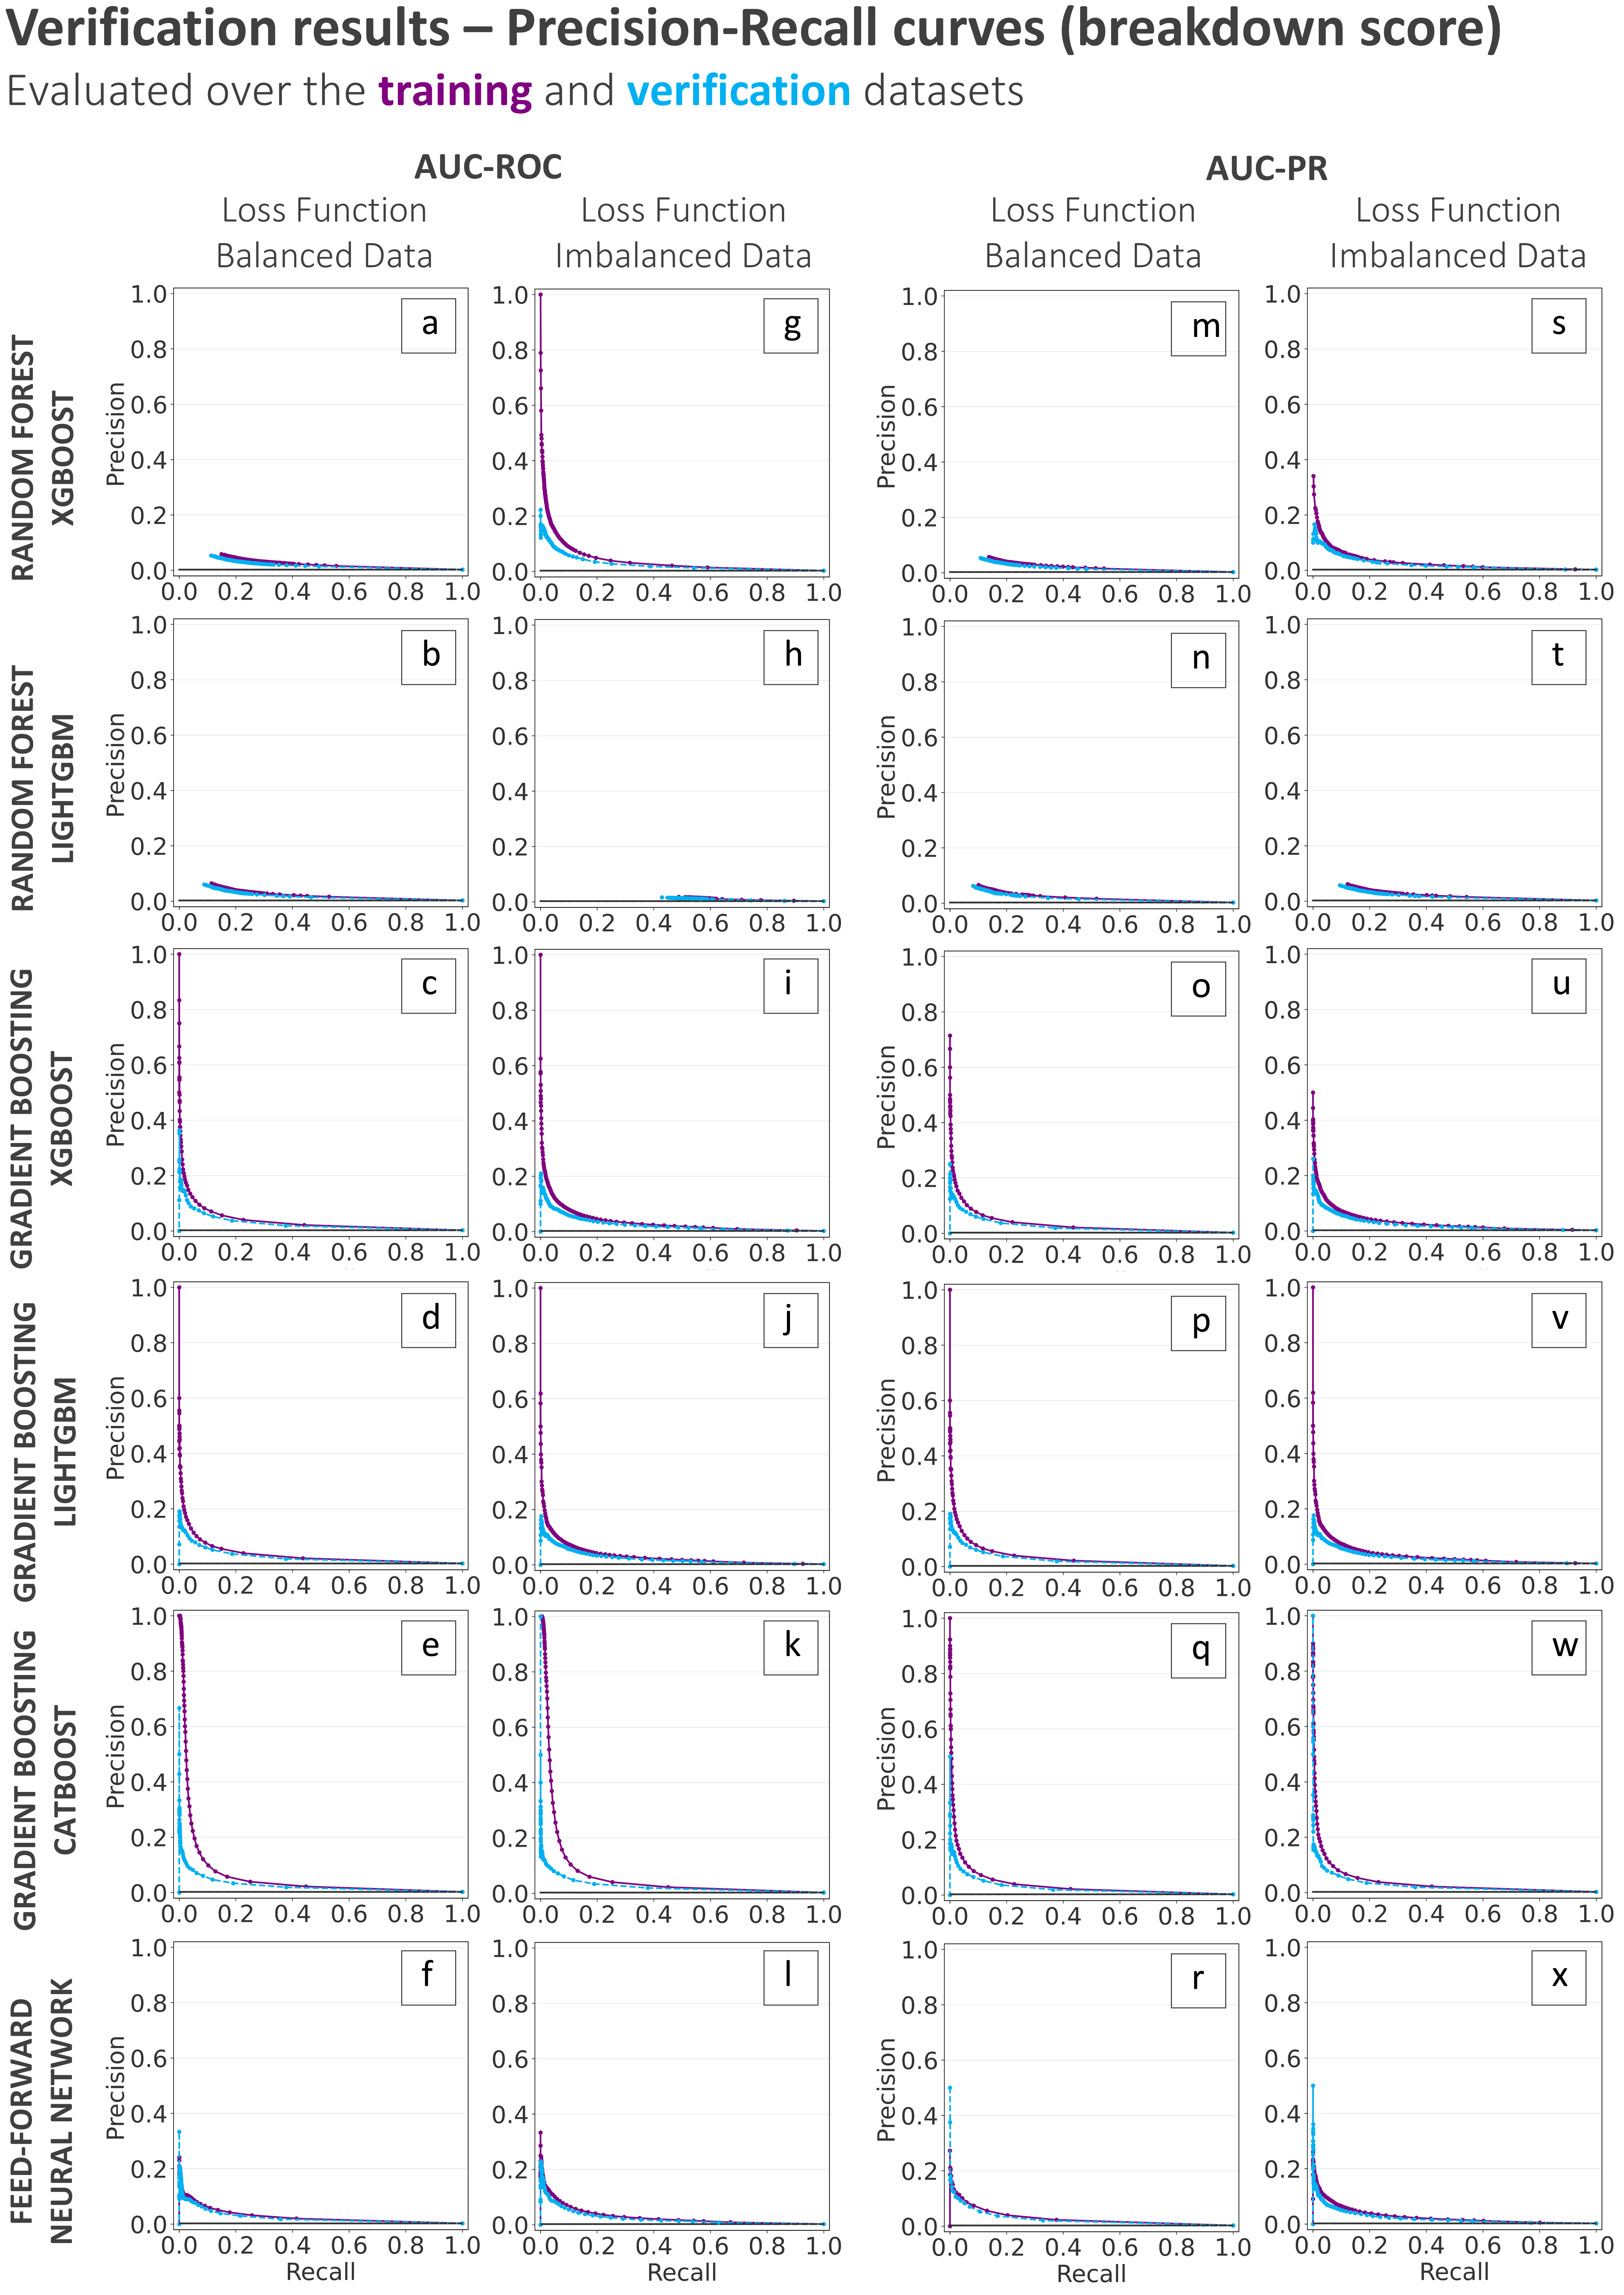
\includegraphics[width=12cm]{figures/verif_training_test_breakdown_pr_curve.png}
\caption{\textbf{Verification results: breakdown scores (Precision-Recall curves)} Similar to Figure \ref{fig:verif_training_test_breakdown_roc_curve} but for the Precision-Recall curve} 
\label{fig:verif_training_test_breakdown_pr_curve}
\end{figure*}

Overall, the reliability diagrams exhibit minimal degradation between \textcolor{colourTraining}{training datasets} and verification datasets, but it increases with increasing forecast probabilities (Figure \ref{fig:verif_training_test_breakdown_reliability_diagram}). Models trained with balanced loss functions (Figures \ref{fig:verif_training_test_breakdown_reliability_diagram}a-f and m-r) demonstrate different calibration characteristics compared to those using weighted loss functions \ref{fig:verif_training_test_breakdown_reliability_diagram}g-l and s-x). For models trained with balanced loss functions, the gradient boosting implementations and the feed-forward neural network yield reliable forecast probabilities under 10\% (20\% for XGBoost). At higher probability ranges, where predictions become less frequent and diagrams noisier, distinct patterns emerge. LightGBM and XGBoost show mostly reliable probabilities across all probability ranges (Figures \ref{fig:verif_training_test_breakdown_reliability_diagram}c-d and o-p). CatBoost systematically underestimates forecast probabilities (Figures \ref{fig:verif_training_test_breakdown_reliability_diagram}e and q). The feed-forward neural network shows contrasting behaviour depending on the evaluation metric used during hyperparameter tuning: overestimation occurs when tuned for AUC-ROC (Figure \ref{fig:verif_training_test_breakdown_reliability_diagram}f), while forecast probabilities remain reliable when tuned considering AUC-PR (Figure \ref{fig:verif_training_test_breakdown_reliability_diagram}r). Models trained with weighted loss functions (Figures \ref{fig:verif_training_test_breakdown_reliability_diagram}g-l and s-x) display systematic overestimation across the entire probability spectrum, except for CatBoost, which maintains similar calibration patterns to its balanced function counterpart. Random forest implementations show systematic overestimations independent of the considered loss function \ref{fig:verif_training_test_breakdown_reliability_diagram}a-b, g-h, m-n, and s-t).

%f
\begin{figure*}[t]
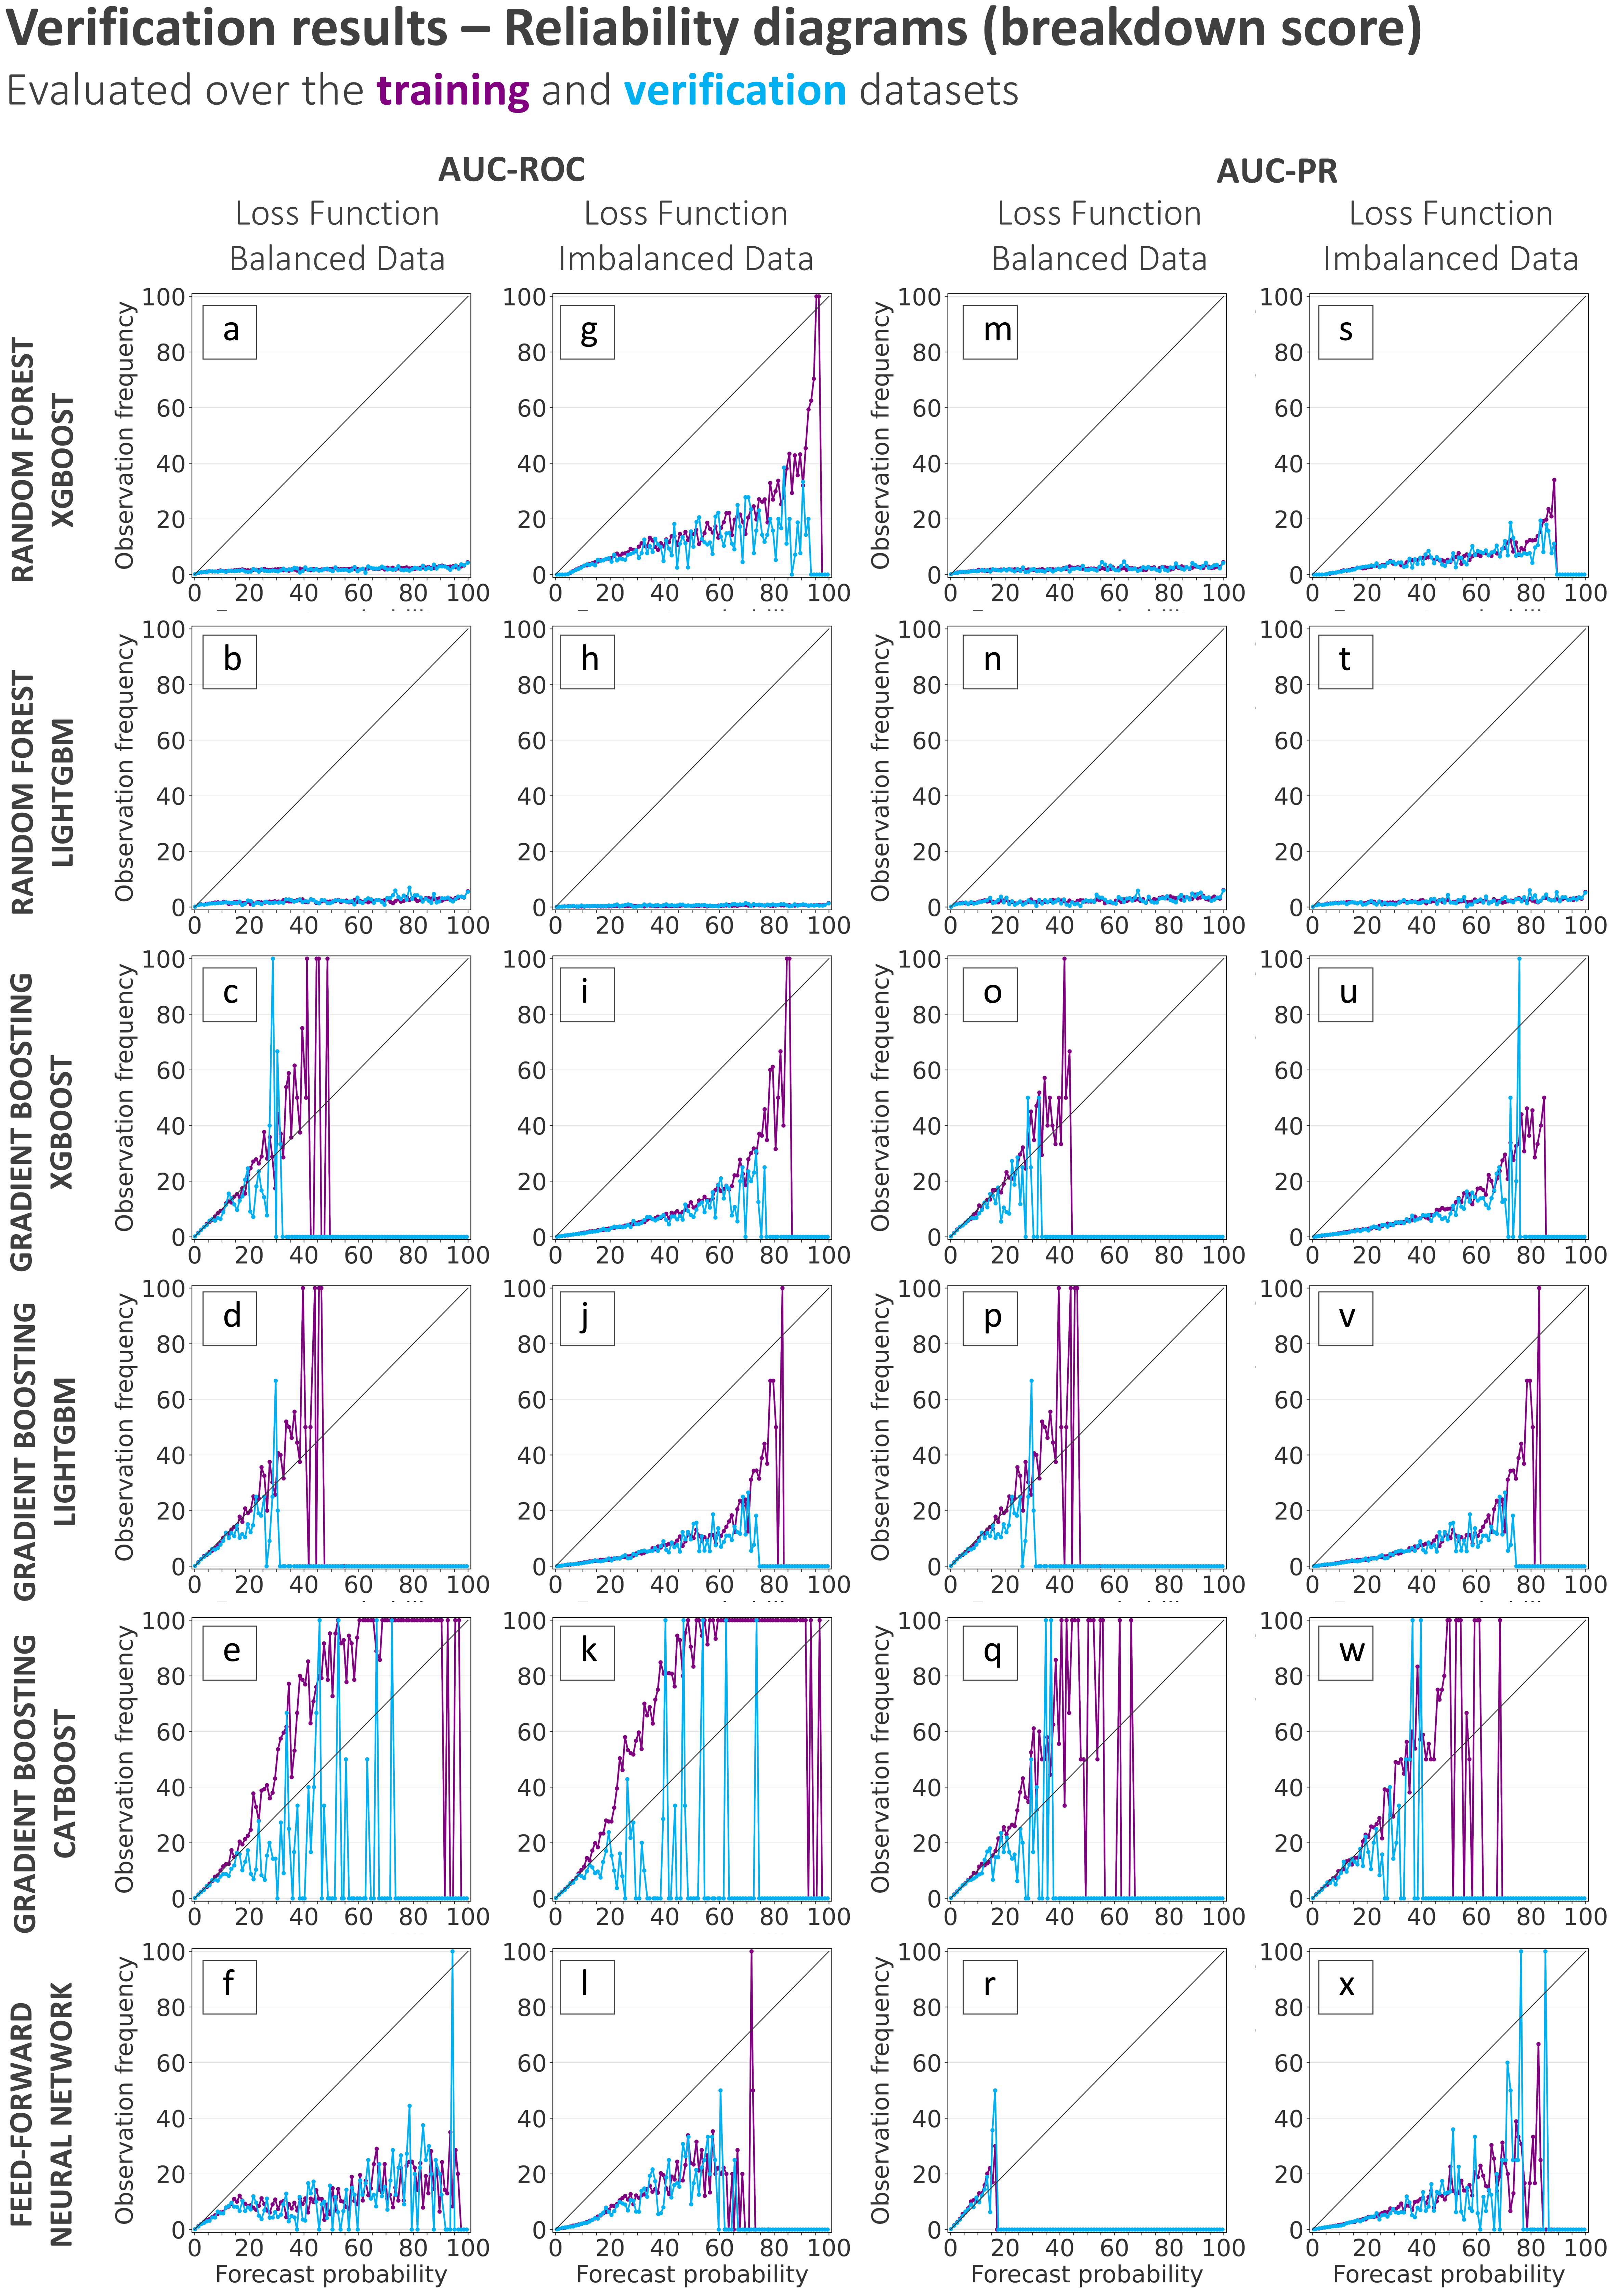
\includegraphics[width=12cm]{figures/verif_training_test_breakdown_reliability_diagram.png}
\caption{\textbf{Verification results: breakdown scores (Reliability diagrams).} Similar to Figure \ref{fig:verif_training_test_breakdown_roc_curve} but for reliability diagrams.}
\label{fig:verif_training_test_breakdown_reliability_diagram}
\end{figure*}


\subsection{Verification results over forecast data}

The area under the ROC curve (AUC-ROC, Figure \ref{fig:verif_long_fc}a) and the area under the precision-recall curve (AUC-PR, Figure \ref{fig:verif_long_fc}b) show a very close performance at day 1 (t+24) to that achieved over the reanalysis data (refer to Figure \ref{fig:verif_training_test_overall}), and it gradually diminishes with increasing lead times. The frequency bias (FB) also slightly deteriorated with increasing lead times, but at day one (t+24), it shows a value that is twice the one obtained for the reanalysis data. 

The ROC curve for day 1 forecasts (t+24, Figure \ref{fig:verif_long_fc}d) also shows a very similar behaviour to that for reanalysis data (refer to Figure \ref{fig:verif_training_test_breakdown_roc_curve}), and shows a fairly small deterioration over increasing lead times (Figure \ref{fig:verif_long_fc}e-f). The precision-recall curve for day 1 forecasts (Figure \ref{fig:verif_long_fc}g) also shows a very similar behaviour to that for reanalysis data (refer to Figure \ref{fig:verif_training_test_breakdown_pr_curve}), except for very small values of recall, where in the precision-recall curve built for the reanalysis data the precision is double. As in the ROC curve, the precision-recall curves also show only a fairly small deterioration over increasing lead times (Figure \ref{fig:verif_long_fc}h-i). As in the two previous scores, also the reliability diagram for day 1 forecasts (Figure \ref{fig:verif_long_fc}j) shows a similar behaviour to that computed for reanalysis data (refer to Figure \ref{fig:verif_training_test_breakdown_reliability_diagram}), with reliable probabilities for forecast probabilities under 10\%. For increasing lead times, such a threshold reduces to ~2\%. For greater probabilities, the reliability diagrams tend to overestimate the observed frequencies of areas at risk of flash floods. 

%f
\begin{figure*}[t]
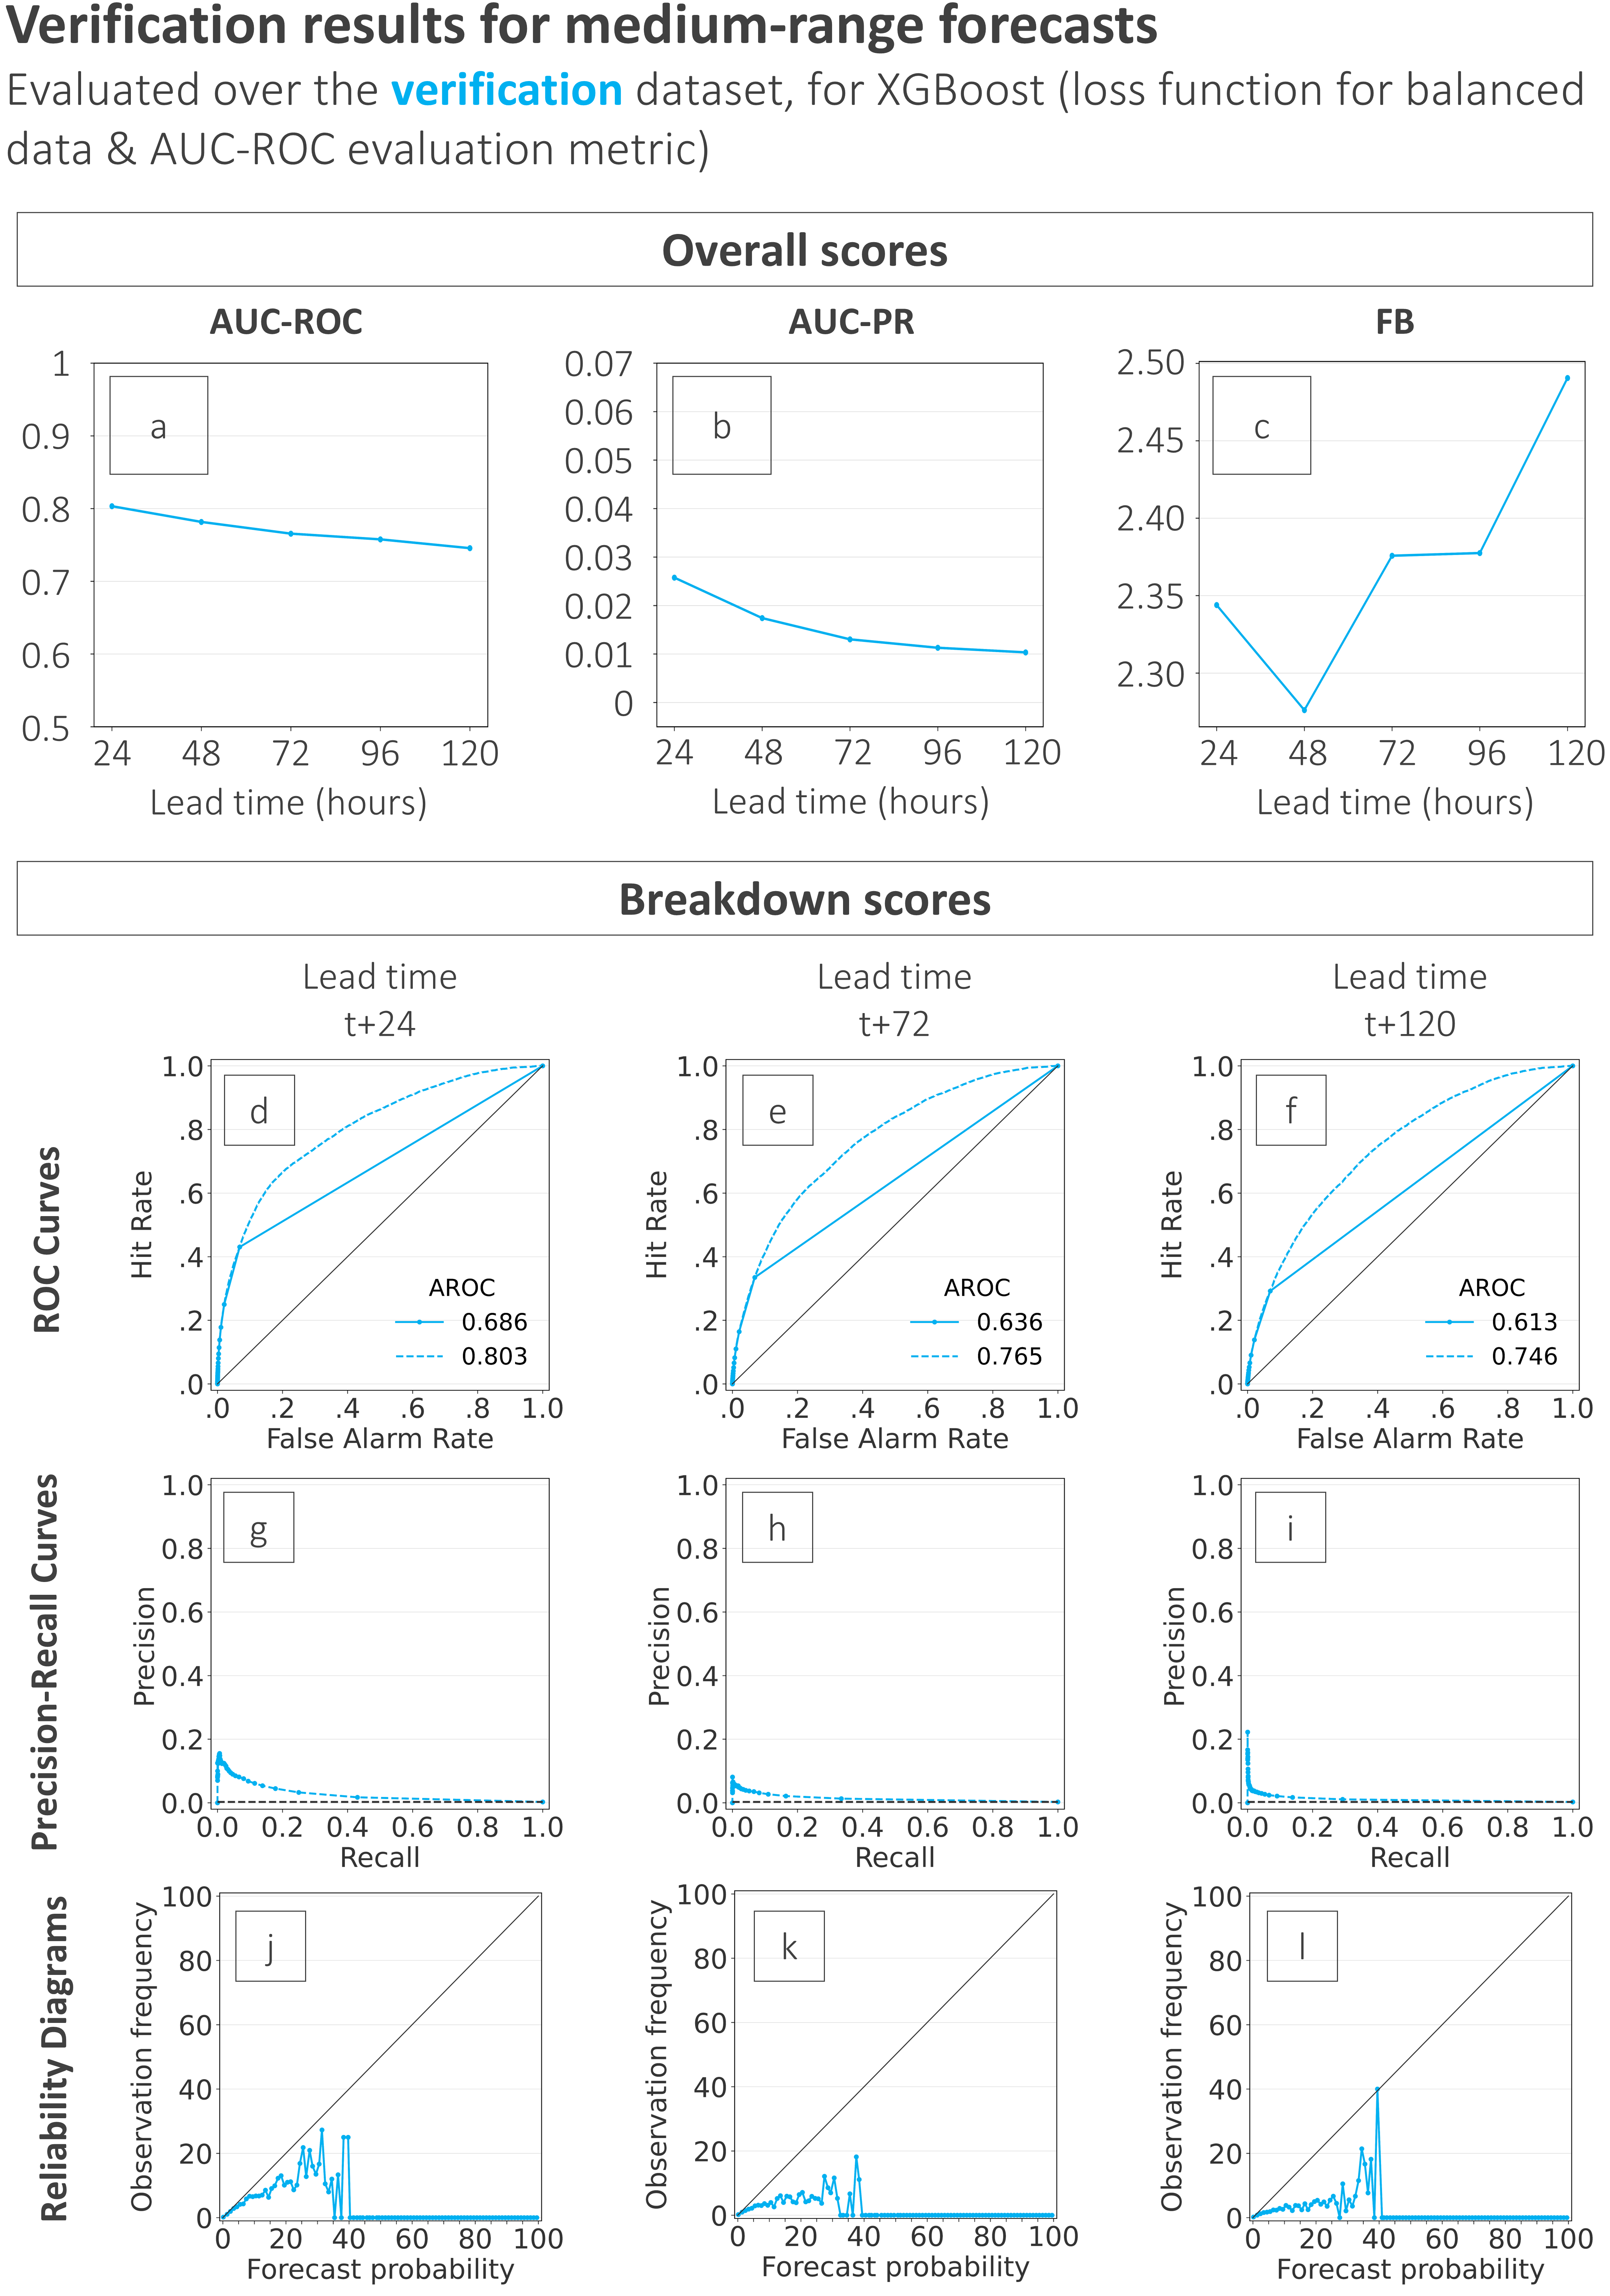
\includegraphics[width=12cm]{figures/verif_long_fc.png}
\caption{\textbf{Verification results for medium-range forecasts for the XGBoost implementation of gradient boosting (trained with the loss function for balanced data and hyperparameters maximised for AUC-ROC).} Panels (a) to (c) show the overall scores, respectively, for the area under the ROC curve (AUC-ROC), the area under the precision-recall curve (AUC-PR), and the frequency bias (FB). The remaining panels show the breakdown scores, respectively, for the ROC curves (Panels (d) to (f)), the Precision-Recall curves (Panels (g) to (i)), and for the Reliability Diagram (Panels (j) to (l)).}
\label{fig:verif_long_fc}
\end{figure*}


%%%%%%%%%%%%%%%%%%%%%%%%%%%%%%%%%%%%%%%%%%%%%%%%%%%%%%%%%%%%%%%%%%%%%%%
\section{Physical interpretation of the data-driven model behaviour}
\label{data_driven_flash_floods_short_medium_range_physical_interpretation}

For the sake of brevity and clarity, the following section will present SHAP-related plots exclusively for the XGBoost implementation of gradient boosting, trained with the balanced loss function and optimised for AUC-ROC. This representative configuration was selected because the feature importance patterns and SHAP value distributions are fairly consistent across all models, loss functions, and evaluation metrics examined in this study. 

%f
\begin{figure*}[t]
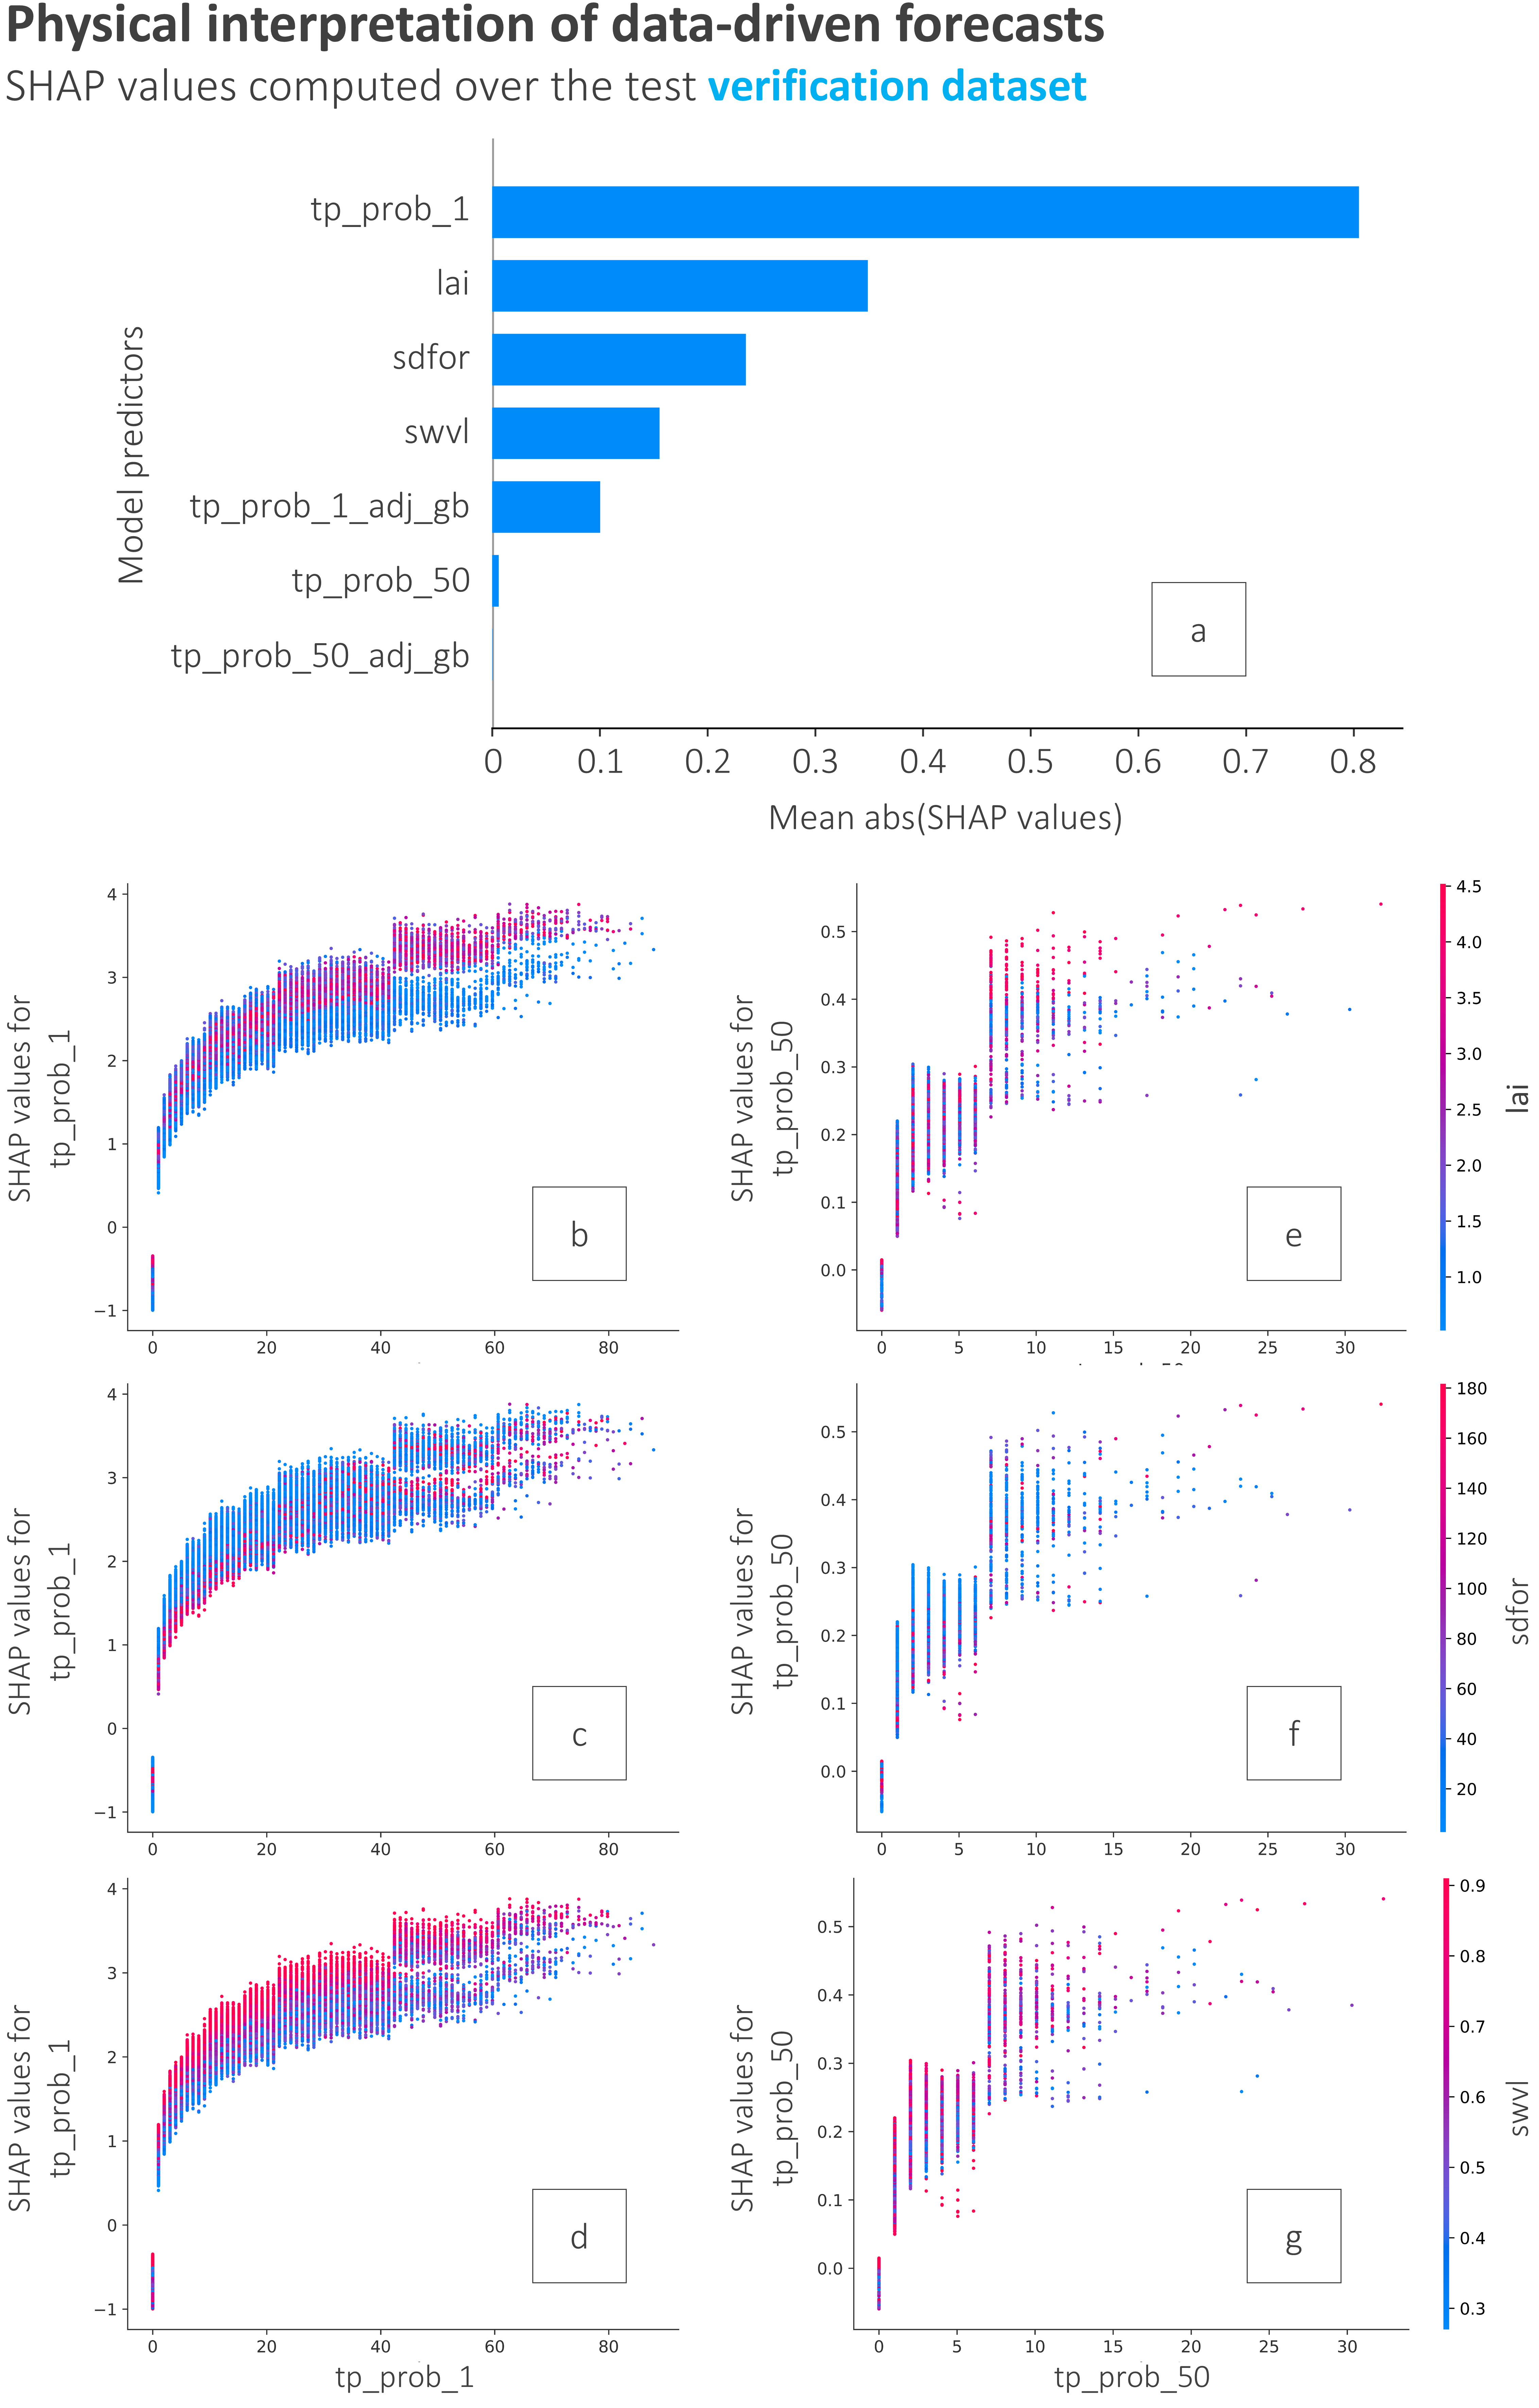
\includegraphics[width=12cm]{figures/shap.png}
\caption{\textbf{SHAP ((SHapley Additive exPlanations)) values over the \textcolor{colourTest}{verification dataset} for the  XGBoost implementation of gradient boosting (trained with the loss function for balanced data and hyperparameters maximised for AUC-ROC).} Panel (a) shows the global feature importance ranking (most important features in descending order). Panels (b) to (d) show the dependency plots between \textit{tp\_prob\_1} and, respectively, \textit{lai}, \textit{sdfor}, and \textit{swvl}. Panels (e) to (g) show the same, but for \textit{tp\_prob\_50.}}
\label{fig:shap}
\end{figure*}

The global feature importance ranking (Figure \ref{fig:shap}a) shows that the rainfall variable for the probability of exceeding the 1-year return period emerges as the most important feature to identify areas at risk of flash flood, contributing to the 80\% of the mean absolute SHAP values. Features regarding the vegetation cover (lai), the orography steepness (sdfor), the antecedent soil moisture (swvl), and the rainfall probabilities of exceeding the 1-year return period in adjacent grid-boxes are also considered important by the model, contributing to 10 to 35\% of the mean absolute SHAP values. The features related to the rainfall probabilities of exceeding the 50-year return period (\textit{tp\_prob\_50} and \textit{tp\_prob\_50\_adj\_gb}) are considered, overall, least important by the model to identify areas at risk of flash flood. 

The dependency plots show critical threshold behaviours in the model's decision-making process. The rainfall-related feature \textit{tp\_prob\_1} (Figure \ref{fig:shap}b-d) contributes positively to the probabilities of having a flash flood in a grid-box. This contribution increases rapidly (from 0 to +3\%) from probabilities between 0\% and ~40\%. For greater probability values (>40\%), the contribution of the rainfall parameters plateaus. For the rainfall-related feature \textit{tp\_prob\_50} (Figure \ref{fig:shap}e-g), the behaviour is similar, but the threshold at which the contributions to the SHAP values plateau reduces to ~7\%. The interactions of the rainfall-related variables with other features (expressed through colour gradients) demonstrate that environmental conditions modify the contributions of rainfall in predicting areas at risk of flash floods. Areas with dense vegetation coverage (higher \textit{lai} values, Figures \ref{fig:shap}b and e), primarily flatter (lower \textit{sdfor} values, Figures \ref{fig:shap}c and f), and with mostly saturated soils (higher \textit{swvl values}, Figures \ref{fig:shap}d and g) enhance sensitivity to rainfall, meaning that lower values of \textit{tp\_prob\_1} are required to trigger higher (positive) SHAP contributions in the probability of having a flash flood in a grid-box.


%%%%%%%%%%%%%%%%%%%%%%%%%%%%%%%
\section{Case Study: Storm Ida}
\label{flash_flood_focused_verification_rainfall_based_ff_CASE_STUDY}

For comprehensive details on Ida's synoptic history, rainfall patterns, and impacts, please refer to Section \ref{datasets_case_study} in Chapter \ref{datasets}.

%f
\begin{figure*}[t]
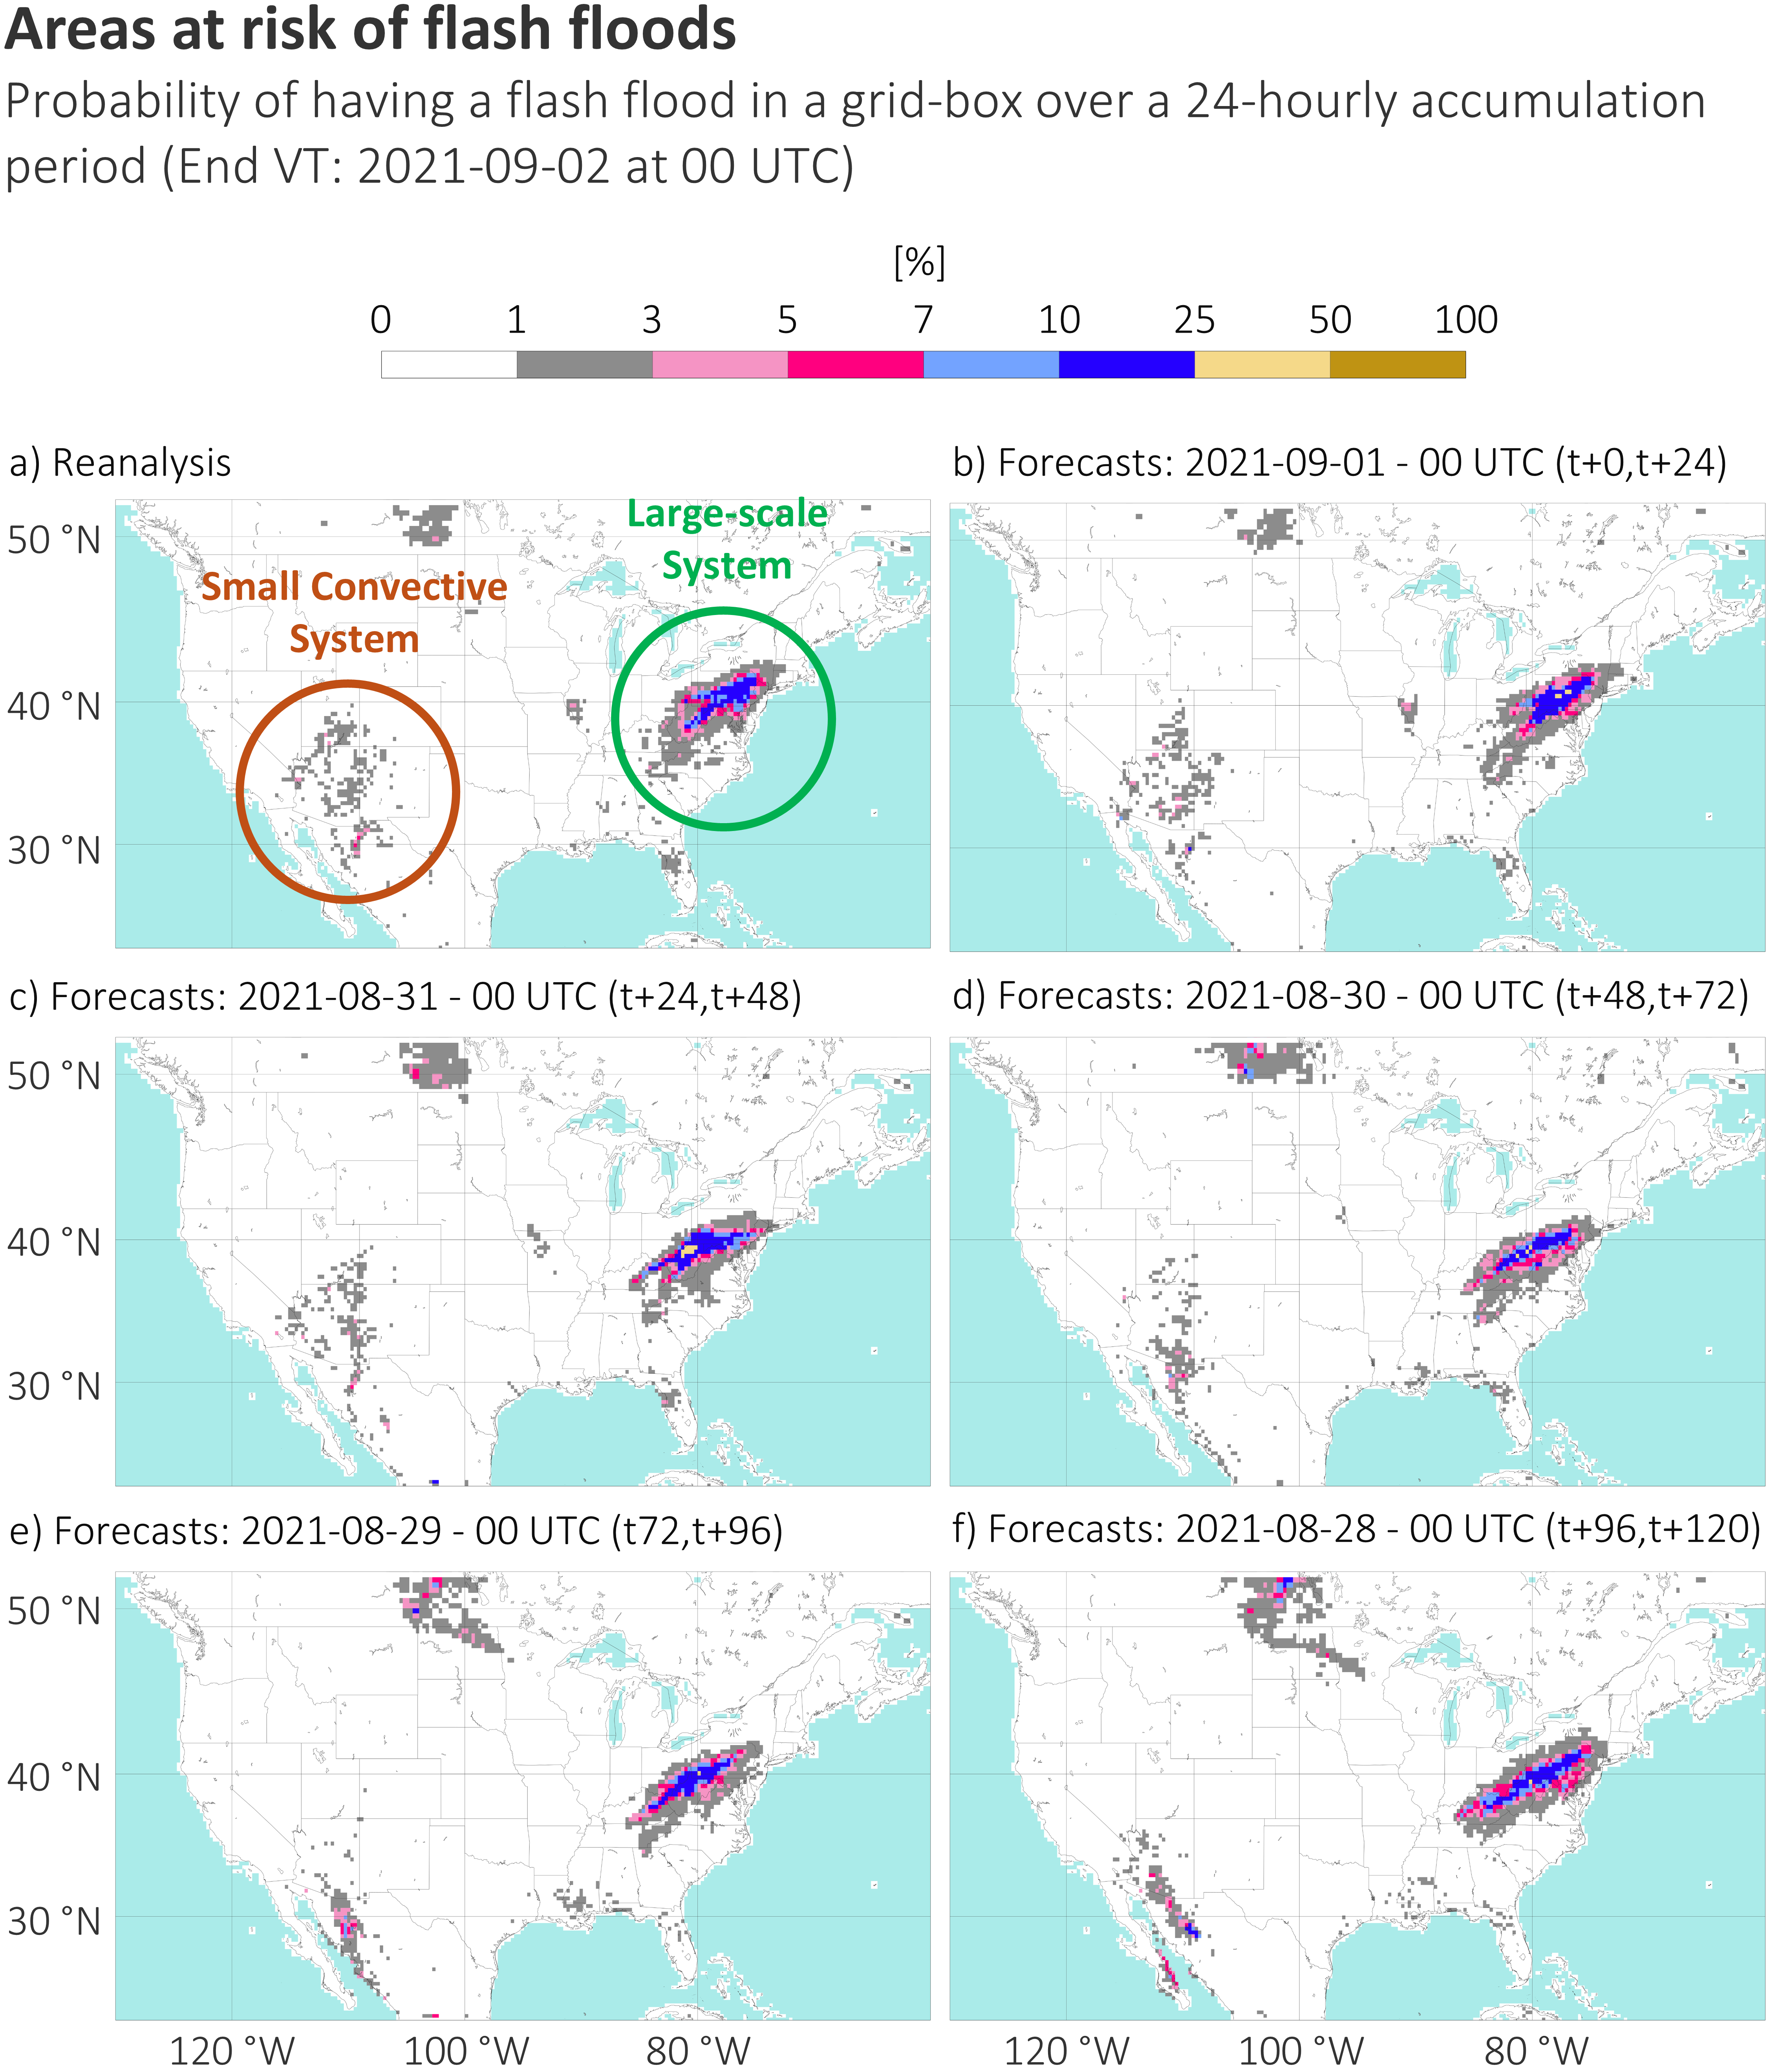
\includegraphics[width=12cm]{figures/case_study_poff.png}
\caption{Probability of having a flash flood in a grid-box, valid for the 24-hourly accumulation ending on 2021-09-02 at 00 UTC. Panel (a) shows the probabilities computed with reanalysis data, while panels (b) to (f) show the probabilities computed with forecast (FC) data, respectively for day 1 (FC: 2021-09-01 at 00 UTC (t+0,t+24)), day 2 (FC: 2021-08-31 at 00 UTC (t+24,48), day 3 (FC: 2021-08-30 at 00 UTC (t+48,t+72), day 4 (FC: 2021-08-29 at 00 UTC (t+72,t+96), and (FC: 2021-08-28 at 00 UTC (t+96,t+120).}
\label{fig:case_study_poff}
\end{figure*}

The model used for the case study is the same as that used in Sections \ref{data_driven_flash_floods_short_medium_range_results_forecasts} and \ref{data_driven_flash_floods_short_medium_range_physical_interpretation}. 
Figure \ref{fig:case_study_poff} illustrates the estimates of areas at risk of flash flood with reanalysis data (Figure \ref{fig:case_study_poff}a) and the evolution of the predictions up to day 5 forecasts (Figures \ref{fig:case_study_poff}b-f). Two different events are highlighted: one due to small convective systems (with the brown circle in Figure \ref{fig:case_study_poff}a) and one due to a large convective system, i.e. Storm Ida (with the brown green circle). The estimates of areas at risk of flash floods, computed using the reanalysis data, can identify the areas where flash floods were reported in the Storm Event Database. The areas at risk of flash floods affected by the large-scale system exhibit high probabilities of experiencing a flash flood (>10\%), and these probabilities are consistently maintained up to medium-range predictions. On the contrary, over the area affected by the small convective system, the probabilities of experiencing a flash flood are much smaller (on average between 1 and 3\%) and more scattered. The signal for the overall area affected can be seen from day 3 (t+72).


%%%%%%%%%%%%%%%%%%%%%
\section{Discussions}
\label{data_driven_flash_floods_short_medium_range_discussions}

The research presented in this chapter provides several insights that enhance the understanding of both the predictive capabilities and operational limitations of machine learning approaches in predicting areas at risk of flash floods. 

The comprehensive model training - carried out through the nested stratified cross-validation approach - and the comparison of different data-driven models provide interesting insights into the required model complexity to achieve good performance in predicting areas at risk of flash flood and how the use of severely imbalanced observational datasets may affect model training and forecast performance. Despite theoretical advantages in capturing non-linear relationships, the feed-forward neural network demonstrates no systematic superiority over tree-based methods, whilst requiring approximately 40 times longer training time. Gradient boosting implementations, particularly XGBoost, emerge as optimal choices, combining competitive performance with computational efficiency and interpretability. The hyperparameter importance analysis reveals that model performance depends primarily on fundamental architectural choices rather than sophisticated optimisation techniques. For gradient boosting methods, maximum tree depth and learning rate consistently dominate, whilst neural networks show the highest sensitivity to first-layer configuration. This finding suggests that, for example, if neural networks must be used, shallow neural networks might be preferred over deeper architectures, as the former is already able to capture the fundamental relationships between predictors and observations, thereby successfully identifying areas at risk of flash floods. In the case of gradient boosting, practitioners should prioritise careful selection of core architectural parameters over extensive hyperparameter search spaces. Finally, the comparative evaluation of balanced versus weighted loss functions reveals fundamental trade-offs in rare event prediction. Models employing weighted binary cross-entropy successfully enhance the identification of areas at risk of flash floods, achieving hit rates approaching 90\% for gradient boosting implementations (compared to 40\% in the case of using loss functions designed for more balanced datasets). However, this enhanced detection comes at the substantial cost of false alarm rates exceeding 50\%, representing a twenty-fold increase compared to balanced configurations. This dramatic increase in false alarms has profound implications for operational deployment. Emergency management systems must strike a balance between the imperative to protect lives through early warning and the risk of warning fatigue from excessive false alarms. These results suggest that for flash flood prediction, where public trust and response compliance are critical, the conservative approach of balanced loss functions may be preferable despite lower identification rates. The frequency bias and reliability diagrams support this conclusion, showing that balanced models provide more reliable predictions.

The evaluation of six distinct machine learning architectures reveals good overall discrimination ability - with all models achieving AUC-ROC values clustering around 0.8 - and acceptable reliability - with all models achieving good reliability for probabilities less than 20\% and overall frequency bias around 1. The AUC-PR metric reveals more nuanced performance variations, with values ranging from 0.02 to 0.03 across most models. Whilst these values appear modest, they represent meaningful skill when put into the context of the climatological frequency of flash floods in the observational dataset, i.e., 0.27\% (0.0027). The precision-recall analysis exposes critical differences between architectures, with gradient boosting implementations and the feed-forward neural network maintaining higher precision at low recall thresholds compared to random forests, which exhibit delayed recall onset requiring extreme threshold relaxation to achieve any sensitivity. The minimal degradation between training (2001-2020) and verification (2021-2024) datasets also demonstrates a good model generalisation, indicating that the learned patterns capture fundamental hydro-meteorological relationships rather than data-specific anomalies.

The analysis of forecast skill degradation of estimates of probabilities of having a flash flood in a grid-box computed with reanalysis data to medium-range predictions (from day 1 to day 5) shows the predictability limits of the data-driven predictions of probabilities of having a flash flood event in a specific area. The discrimination ability, as estimated by the ROC curves and the AUC-ROC, shows a minimal degradation over time - from ~0.8 to ~0.75. On the contrary, the AUC-PR exhibits steeper degradation from ~0.025 to ~0.01, reflecting the increasing difficulty for the forecasts in maintaining precision for rare event detection as forecast uncertainty compounds. The reliability diagrams confirm that while low-probability predictions (<10\%) maintain reasonable reliability at short lead times (for reanalysis data and day 1 forecasts), this threshold reduces considerably (<2\%) beyond day 2.

The SHAP analysis establishes a clear hierarchy of predictive features that generally aligns with hydrological understanding. The overwhelming dominance of the rainfall parameter (\textit{tp\_prob\_1}), accounting for 80\% of mean absolute SHAP values, confirms that rainfall remains the primary driver of flash flood occurrence. The secondary features demonstrate modulating effects on the influence that the rainfall parameter has in enhancing the probability of a flash flood event. However, there is no always complete alignment with the general hydrological understanding of their impact on flash flood occurrence. The vegetation coverage parameter (\textit{lai}) emerges as the second most influential parameter in determining the probability of a flash flood event. In flash flood susceptibility studies, vegetation parameters do not rank as high as in this study. Moreover, such parameters suggest that it is the lack of vegetation that increases the risk of flash flood occurrence. In contrast, these results indicate that the probability of having a flash flood increases with large values of LAI, which suggests dense vegetation. This odd correlation might be due to the fact that, climatologically, lai values are greater over the summer \citep{Owens_2018}. The Storm Event Database indicates that, climatologically, flash flood events occur primarily during the summer, as this is when most convective flash-flood-triggering rainfall events occur \citep{Davis_2001}. Thus, this unusual behaviour regarding the vegetation coverage parameter may be due to the relationship between its highest values occurring over the same season as the highest frequency of flash floods occurs. More investigation is, therefore, needed to confirm this explanation, and if it is correct, engineer or substitute the lai parameter to represent only vegetation coverage, with no secondary relationships to rainfall to avoid double counting. After the vegetation coverage, the most important parameters influencing the probabilities of having a flash flood event are topographic steepness (\textit{sdfor}) and antecedent soil moisture (\textit{swvl}). This ranking agrees with flash flood susceptibility studies. The analysis of SHAP values suggests that high water content in the soil does modulate the effect of rainfall in defining the probabilities of having a flash flood event, i.e., the same amount of rainfall over a saturated soil increases the chances of having a flash flood event, compared to the case the same rainfall amount falls over dry soil. This agrees of our understanding of the modulating effects of soil water content of the effects that different rainfall amounts might have in the generation of flash flood events. On the contrary, the results provided by the SHAP values regarding the steepness of the orography provide an opposite of what physical hydrology suggests. The analysis of SHAP values suggests that primarily small values of sdfor (flatter areas) increase the probability of having a flash flood event. This contrasting result with physical hydrology may be due to where impact flash flood reports tend to be located. While it is known that flood water rises rapidly in complex orographic areas, the majority of the impacts are seen in the valleys, downstream of the complex orographic areas, where typically most of the people live and where the majority of the impacts are reported. It is, therefore, assumed that this odd relationship with the orographic parameters is the result of the type of observational dataset considered in this analysis (impact reports) rather than a genuine physical relationship, and that this result might change if discharge observations were considered instead. 

Based on the comprehensive evaluation across training, verification, and case study analyses, the XGBoost implementation of gradient boosting trained with balanced loss function and optimised for AUC-ROC emerges as the recommended configuration for operational deployment. This recommendation rests on multiple converging lines of evidence that address both technical performance and practical constraints. The selected configuration maintains stable AUC-ROC around 0.8 and high AUC-PR values (from ~0.03 and 0.01) across lead times. The XGBoost implementation of gradient boosting also shows frequency bias closest to 1 when probabilities are computed with reanalysis data and stable around 2.5 when forecasts up to medium-range lead times are considered. It is also the architecture that maintains good reliability for the highest probability threshold when considering reanalysis data (< 10\%) and forecasts (< 2\%). The case study supports this choice, demonstrating a good correspondence in XGBoost between predictions of areas at risk of flash floods and observations, without the noisy patterns exhibited in other models (not shown), which produce a high number of grid-boxes with probabilities between 1 and 3\% in areas where there were no records of flash flood events. Finally, from a computational perspective, XGBoost's training time of approximately 20 minutes per fold enables regular model updates as new event reports become available. LightGBM and CatBoost also appear as good options. However, CatBoost has a significantly longer training time than XGBoost and LightGBM (i.e., 2 hours), which may make it less suitable for operational applications.


\conclusions 
This chapter has demonstrated the feasibility of developing data-driven predictions of flash flood risk at regional scales using hydro-meteorological reanalysis data and impact reports, successfully addressing Research Question 2 of this thesis. 

The comprehensive evaluation of six machine learning architectures reveals that gradient boosting implementations, particularly XGBoost, achieve optimal performance in predicting areas at risk of flash floods over the CONUS. Shallow neural networks achieve a similar performance but at a 40 times higher training cost (8 hours rather than 20 minutes), which may make it less palatable for operational implementations. 

The integration of hydrological features (e.g., soil moisture, vegetation indices, and topographic characteristics) beyond only precipitation variables (as seen in Chapter \ref{flash_flood_focused_verification_rainfall_based_ff}) enhances predictive capabilities. While the SHAP analysis confirms that 1-hour precipitation probability dominates model decisions with an 80\% contribution, hydrological, climatological, and static features critically modulate the impact of the rainfall variables in predicting areas at risk of flash flood.

Skill degradation analysis establishes clear operational protocols. High-confidence warnings between 0-24 hour forecasts may be used for taking (high-cost) protective actions such as evacuation of people, while less confident forecasts (lead times > t+24) may be used for (low-cost) preparedness actions such as moving belongings to higher floors or strategic planning such as calling people to monitor possible flash flooding situation and be ready to take actions. 

While this development uses rainfall forecasts post-processed with the ecPoint methodology (which produces rainfall estimates at point-scale), future research should prioritise integration with higher-resolution global NWP models (e.g. IFS at 9 km) or with convection-permitting models (e.g. Destination Earth implementations at 4 km resolution) to better capture localised hydro-meteorological processes, addressing current limitations of 31-kilometre grids. While this study provides probabilities of areas at risk of flash floods and utilises model architectures such as random forest and gradient boosting, which are considered ensemble models, the model outputs can be considered deterministic because only one probability value is provided per model. Ensemble approaches, such as bagging and stacking, which combine multiple data-driven architectures, could provide robust uncertainty quantification essential for operational forecasting. The models developed here are valid over the CONUS, but could potentially be run operationally using global NWP model output and produce predictions over a continuous global domain. However, the best approach to do this remains to be assessed.


%% ---------------------------------

\codedataavailability{All code, raw and processed data can be provided by the corresponding author upon request.} %% use this section when having data sets and software code available

\authorcontribution{F.M.P. designed the research, developed the model code, performed the simulations, analysed the data, plotted the graphs, and wrote the manuscript. M.C., F.P., C.P., and H.L.C. supervised the study, reviewed and edited the manuscript.} 

\competinginterests{The authors have no competing interests to declare,} 

\begin{acknowledgements}
This research is part of the PhD project titled “Outrunning flash floods: improving global medium-range forecasts for better preparedness” within the Doctoral Course “A.D.I.” at the University of Reading.
\end{acknowledgements}


%% References
\bibliographystyle{copernicus}
\bibliography{references.bib}


%% FIGURES

%% When figures and tables are placed at the end of the MS (article in one-column style), please add \clearpage
%% between bibliography and first table and/or figure as well as between each table and/or figure.

% The figure files should be labelled correctly with Arabic numerals (e.g. fig01.jpg, fig02.png).


%% ONE-COLUMN FIGURES

%%f
%\begin{figure}[t]
%\includegraphics[width=8.3cm]{figures/}
%\caption{TEXT}
%\end{figure}
%
%%% TWO-COLUMN FIGURES
%
%%f
%\begin{figure*}[t]
%\includegraphics[width=12cm]{figures/}
%\caption{TEXT}
%\end{figure*}
%
%
%%% TABLES
%%%
%%% The different columns must be seperated with a & command and should
%%% end with \\ to identify the column brake.
%
%%% ONE-COLUMN TABLE
%
%%t
%\begin{table}[t]
%\caption{TEXT}
%\begin{tabular}{column = lcr}
%\tophline
%
%\middlehline
%
%\bottomhline
%\end{tabular}
%\belowtable{} % Table Footnotes
%\end{table}
%
%%% TWO-COLUMN TABLE
%
%%t
%\begin{table*}[t]
%\caption{TEXT}
%\begin{tabular}{column = lcr}
%\tophline
%
%\middlehline
%
%\bottomhline
%\end{tabular}
%\belowtable{} % Table Footnotes
%\end{table*}
%
%%% LANDSCAPE TABLE
%
%%t
%\begin{sidewaystable*}[t]
%\caption{TEXT}
%\begin{tabular}{column = lcr}
%\tophline
%
%\middlehline
%
%\bottomhline
%\end{tabular}
%\belowtable{} % Table Footnotes
%\end{sidewaystable*}
%
%
%%% MATHEMATICAL EXPRESSIONS
%
%%% All papers typeset by Copernicus Publications follow the math typesetting regulations
%%% given by the IUPAC Green Book (IUPAC: Quantities, Units and Symbols in Physical Chemistry,
%%% 2nd Edn., Blackwell Science, available at: http://old.iupac.org/publications/books/gbook/green_book_2ed.pdf, 1993).
%%%
%%% Physical quantities/variables are typeset in italic font (t for time, T for Temperature)
%%% Indices which are not defined are typeset in italic font (x, y, z, a, b, c)
%%% Items/objects which are defined are typeset in roman font (Car A, Car B)
%%% Descriptions/specifications which are defined by itself are typeset in roman font (abs, rel, ref, tot, net, ice)
%%% Abbreviations from 2 letters are typeset in roman font (RH, LAI)
%%% Vectors are identified in bold italic font using \vec{x}
%%% Matrices are identified in bold roman font
%%% Multiplication signs are typeset using the LaTeX commands \times (for vector products, grids, and exponential notations) or \cdot
%%% The character * should not be applied as mutliplication sign
%
%
%%% EQUATIONS
%
%%% Single-row equation
%
%\begin{equation}
%
%\end{equation}
%
%%% Multiline equation
%
%\begin{align}
%& 3 + 5 = 8\\
%& 3 + 5 = 8\\
%& 3 + 5 = 8
%\end{align}
%
%
%%% MATRICES
%
%\begin{matrix}
%x & y & z\\
%x & y & z\\
%x & y & z\\
%\end{matrix}
%
%
%%% ALGORITHM
%
%\begin{algorithm}
%\caption{...}
%\label{a1}
%\begin{algorithmic}
%...
%\end{algorithmic}
%\end{algorithm}
%
%
%%% CHEMICAL FORMULAS AND REACTIONS
%
%%% For formulas embedded in the text, please use \chem{}
%
%%% The reaction environment creates labels including the letter R, i.e. (R1), (R2), etc.
%
%\begin{reaction}
%%% \rightarrow should be used for normal (one-way) chemical reactions
%%% \rightleftharpoons should be used for equilibria
%%% \leftrightarrow should be used for resonance structures
%\end{reaction}
%
%
%%% PHYSICAL UNITS
%%%
%%% Please use \unit{} and apply the exponential notation


\end{document}